\documentclass{article}
\usepackage[utf8]{inputenc}
\usepackage{geometry}
\geometry{legalpaper, margin=1in}

\setlength{\parindent}{0pt}
\setlength{\parskip}{1em}

\usepackage{graphicx}
\usepackage{amsmath}
\usepackage{amsfonts}
\usepackage{cancel}
\usepackage{tcolorbox}
\usepackage{appendix}
\usepackage{hyperref}
\hypersetup{
    colorlinks=true,
    linkcolor=blue,
    filecolor=magenta,      
    urlcolor=blue,
}

\usepackage{listings}

\usepackage{color}
\usepackage{xcolor}

\definecolor{codegreen}{rgb}{0,0.6,0}
\definecolor{codegray}{rgb}{0.5,0.5,0.5}
\definecolor{codepurple}{rgb}{0.58,0,0.82}
\definecolor{backcolour}{rgb}{.92,0.92,0.92}
\definecolor{backblue}{cmyk}{0.1, 0.0, 0.0, 0.07, 0.6}

\renewcommand{\ttdefault}{pcr}
\lstdefinestyle{Python}{
    language        = Python,
    basicstyle=\ttfamily\bfseries,
    %keywordstyle    = \color{orange},
    %keywordstyle    = [2] \color{teal}, % just to check that it works
    %stringstyle     = \color{green},
    %commentstyle    = \color{red}\ttfamily,
    backgroundcolor=\color{backcolour},   
    commentstyle=\color{magenta},
    keywordstyle=\color{blue},
    numberstyle=\tiny\color{codegray},
    stringstyle=\color{codegreen},
    identifierstyle=\color{black},
    emph={[4]for,in,def,import}, emphstyle={[4]\color{orange}},
    morekeywords={True,False,as, range},
}



\title{Imperial College HEPP Postgraduate Lectures - Statistics}
\author{Nicholas Wardle }
\date{August 2020}

\begin{document}
\lstset{
    frame       = single,
    numbers     = left,
    showspaces  = false,
    showstringspaces    = false,
    %captionpos  = t,
    %caption     = \lstname
}

\maketitle
\tableofcontents
\section{Ideas for next time}

\begin{itemize}
\item you should move over all of the examples to \textsc{ipynb} format which will be nicer to present - you're doing it already but just carry on. - maybe not the intense ones like frequentist stuff (takes too long in notebooks).

\item Have a section thats just common pdfs. You already show Poissons, also show the chi2 and have a final one of Gaussians. Also in 2D - helpful for correlations 

\item Remove the hypotest with spin-1/spin-0. I don't like it. Replace with something more concrete (like the spin test and use histograms? or a nicer functional form?). Or just create some data for it and do a full test. actually lets do a lifetime example test for b vs c decay and decay distance!

\item I removed gof test. Instead, lets go over the multidim fit and cover things like Hessian and covariance matrix from the likelihood. can c.f chi2 tests if you like. 
Actually lets put it back but use it as another  hypotest example. i will do mdf in 2 D but as asymptotic and compare to the gradient approx ie the chi2 is a quadratic near the minimum, so do that later in intervals.
\end{itemize}


\section{Introduction}

These courses are supposed to give you an overview of the kind of statistical issues you're likely to face during your PhD, when analysing experimental data. Often the kind of issues we high energy physicists deal with are not the same as for statisticians dealing with survey questionnaires, financial traders dealing with index price fluctuations or epidemiologists dealing with viral outbreaks. However, some of the fundamental concepts of course are the same (even if in practise it leads to very different levels of rigour). 

These lectures are therefore not meant to be a complete course in statistics theory, but rather a practical course focused on the most common statistical methods used in HEP. I'm basing a lot of this material on an excellent book by Frederick James, \emph{``Statistical Methods in Experimental Physics: 2nd Edition,''} (see Figure~\ref{fig:james} below). I strongly recommend this book for further reading on statistics for high energy particle physics. 

\begin{figure}[hbt!]
    \centering
    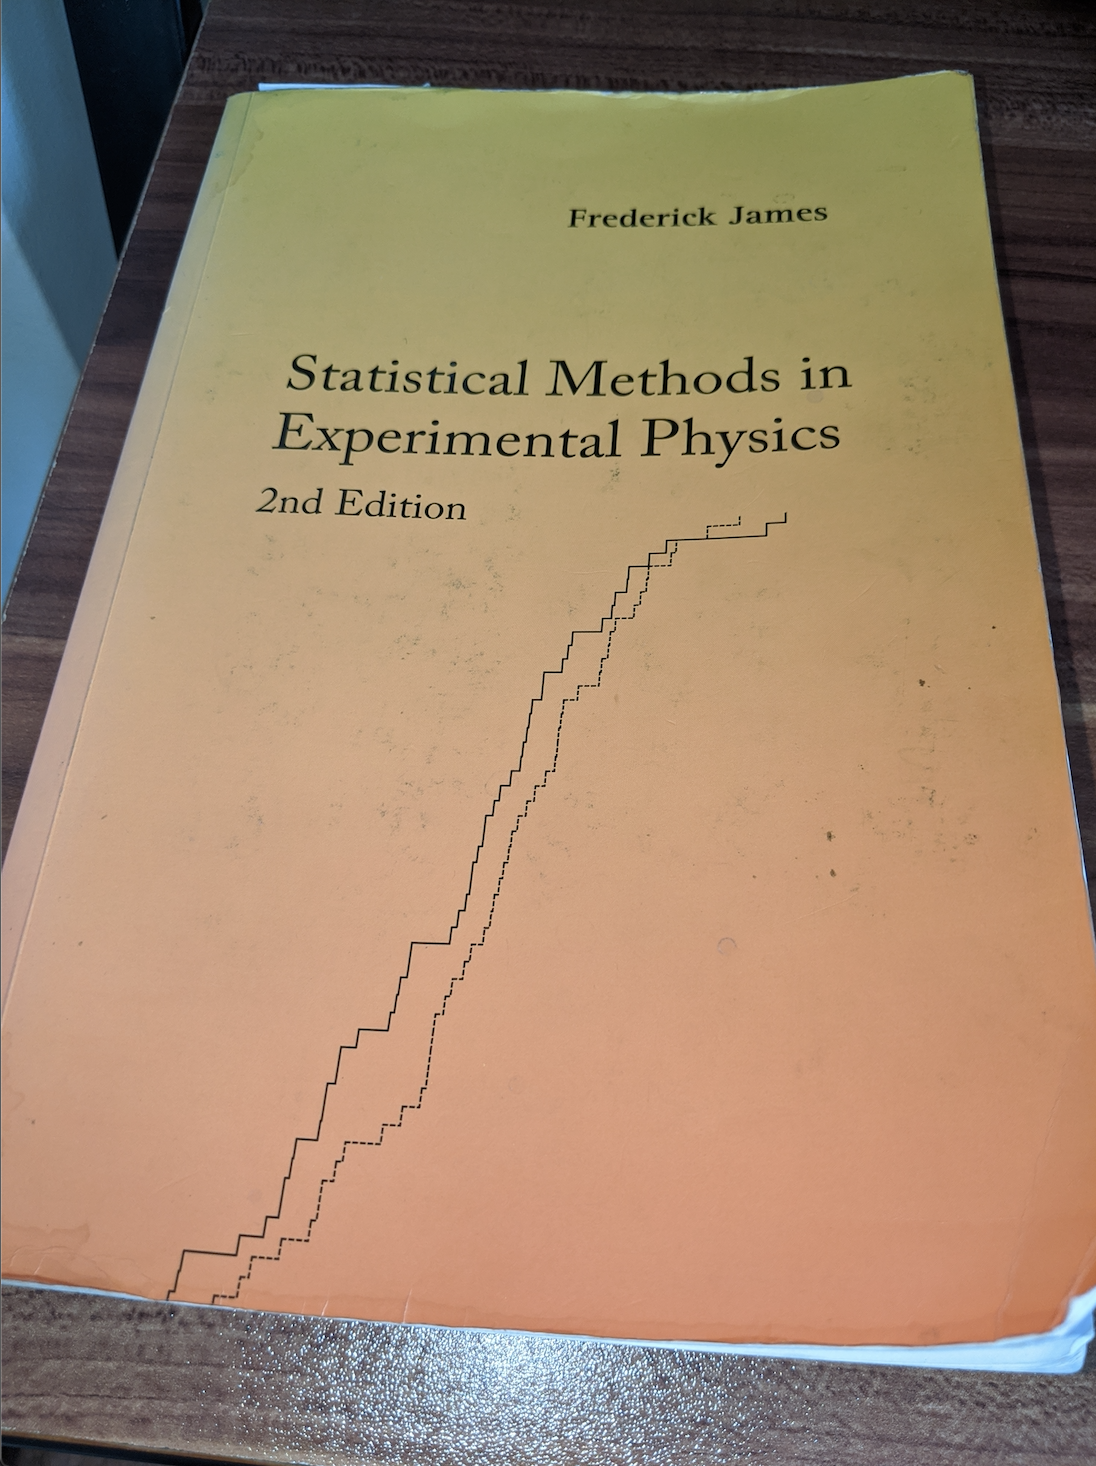
\includegraphics[width=0.5\textwidth]{figures/intro/james.png}
    \caption{My beaten up copy of James, coffee stains and all.}
    \label{fig:james}
\end{figure}

While the theory behind the statistical methods we'll cover is vital to understand what we do and why we do it, the practicality of using those methods is equally important for a successful PhD in HEP. These lectures will include some element of programming to give you an idea as to how to code up the methods for your own research. Since every collaboration/experiment will have their own fitting/statistics software, and since there are many industry standards out there, I'll try to simple code without using too many fancy packages. For the problems, feel free to use whatever you like concerning languages/packages to get the solutions. I'll be interested in seeing what you can come up with. A few examples of good languages for programming statistics are \textsf{R, python, ROOT (C++ based), Mathematica...} and of course there are plenty of tools for complicated statistical routines and workflows such as \textsf{PyTorch, tensorflow, Stan, Minuit (iMinuit), RooFit/RooStats, pyHF, HistFitter/HistFactory, Combine ...}. 
Whenever there is a snippet of code to explain something, you'll see a code box like the following. 

\begin{lstlisting}[style = Python]
# basic Python codeblock
nothing = [print("hello") for i in range(10)]
# or the for loop version
for i in range(10): 
  print("hello")
\end{lstlisting}

I'll tend to use \textsf{python 3}, but you should not let that discourage you from using another language if you prefer. We care about the statistics in the end. All of the code examples in these lectures can be found in full on \textsf{GutHub} at  \url{https://github.com/nucleosynthesis/PGStatistics}. You can follow along by either checking out the repository and running the notebooks (in the  \textsf{notebooks} folder) or launching a python interpreter to run in your browser by either clicking the button that looks like this: 
\includegraphics[height=1.2\fontcharht\font`\B]{figures/binder.png}, or by clicking \href{https://mybinder.org/v2/gh/nucleosynthesis/PGStatistics/main?urlpath=lab}{this link}. 

By the end of this course, you should have an idea of what a particle physicist means by an ``limit'', a ``significant result'' and what is really meant by a ``measured value of  $X+\pm \sigma_{X}$''. Furthermore, you should be able to calculate such things yourself using some simple programming tools.  


\section{Probability}
In this first lecture, we will review the basic concept of \emph{probability}. You probably have a good idea already of what probability is, however the mathematical developed in 1933 by Kolmogorov treats probability as something which satisfies three axioms, and therefore no specific definition is given. The Kolmogorov axioms are, 
\begin{itemize}
    \item $P(X_i)\geq0$ for all $i$
    \item $P(X_i~\mathrm{or}~X_j)= P(X_i) + P(X_j)$ 
    \item $\sum_{\Omega}P(X_i) =1$,
\end{itemize}
where $\Omega$ is the set of all possible, exclusive events $X_i$ and $P(X_i)$ is the probability for $X_i$ to occur. 

We can see that probability should (probably) be at least a real number between 0 and 1, but otherwise we're free to choose the interpretation. For any meaningful statistics, we need a more practical definition and like all great constructs of society (democratic elections, quantum mechanics interpretations and ``who shot first'' in ``Star wars IV: A new hope''), there are only two credible choices. 

\subsection{Frequentist probability}

The concept of probability in the \emph{frequensist} (or classical) paradigm is the one that you are most likely familiar with. As the name suggests, this definition of probability is related to the frequency with which an event occurs in repeated trials. More formally, imagine an experiment in which a series of events is observed and suppose that some ($n$) of these events can be labelled of type $X $. The probability that any single event out of a total number of $N$ events will be of type $X$ is given by the limit of the ratio, 
\begin{equation}
    P(X) = \mathrm{lim}_{N\rightarrow \infty}\frac{n}{N}.
\end{equation}
Note that we inherit some limitations with this interpretation. This concept of probability can only be applied to repeated experiments, meaning the probability only makes sense when describing an ensemble of experiments. Furthermore, the conditions of these experiments must be essentially identical. As physicists, this shouldn't be an issue for you as good science requires reproducible results. On the other hand, this definition is very objective in the sense that if everyone agrees on the definition of $X$, no-one can object to the probability for an event to be labelled $X$ - i.e the probability is independent of who is determining it.  

\subsection{Bayesian probability}

The other commonly used definition of probability is \emph{Bayesian probability}. This definition abandons the concept of frequency and instead defines probability as something which can be applied to non-repeatable experiments. The concept of Bayesian probability is based on the \emph{degree of belief} in an event $X$ occurring. Often, this is described in terms of the odds of winning a bet based on the outcome. Say for example that the odds on $X$ occurring are 4:1, meaning if you place a bet of £1 that $X$ occurs, you could either make a £4 profit or a £1 loss. If you are \emph{willing to take those odds}, as a Bayesian, then you would ascribe a probability $P(X)=1/(4+1)$ -- the ratio between the amount you would bet to the total amount you stand to win (including the original bet) under those odds.  Intuitively this makes sense, since $P(X)$ being very small means that you are almost certain $X$ will not occur and therefore require very high odds before its worth betting any money. Instead $P(X)=0.5$ means that you have have no strong belief about the outcome of $X$ and therefore willing to accept odds of 1:1. 

Note however that this definition of probability is a property of the observer and the system at the same time. It is also not a constant with time. As the observer gains more knowledge (perhaps by playing the game and placing a bet a few times), their value of $P(X)$ will change. This definition of probability is therefore \emph{subjective}. This is not necessarily a bad thing of course. Why shouldn't we update our believe about something after we gain knowledge and if you know more about how and when $X$ will occur than I do, why should your probability be the same as mine? We'll see that this definition of probability has its advantages and at the end of the day, as physicists we want to use the definitions most convenient to the problem at hand. 


\subsection{Properties of probability}

Let's quickly revisit the properties of any quantity that satisfies the Kolmogorov axioms. You would have seen these at school so there's nothing new here (hopefully). Let $P(A)$ be the probability that an exclusive event $X_i$ occurs in $A$. Now consider two non-exclusive sets $A$ and $B$ of exclusive events $X_i$. Then the probability of an event occurring in either $A$, or $B$, or in both is given by, 
\begin{equation}\label{eqn:aorb}
    P(A~\mathrm{or}~B) = P(A)+P(B)-P(A~\mathrm{and}~B),
\end{equation}
where $(A~\mathrm{or}~B)$ denotes the set of events $X_i$ which belong to either set $A$ or set $B$, or both. $(A~\mathrm{and}~B)$ denotes the set of events belonging to both.  
\begin{tcolorbox}[colback=backblue]
\textbf{Example:} Let $A$  be all even rolls of a six-sided die, and $\{X_i\}_1^6$ are the outcomes of a single roll of the die -- i.e $X_1$ denotes that a 1 is rolled, $X_2$ denotes that a 2 is rolled etc. Now let $B$ be all rolls which result in an outcome greater than or equal to 4. Then, according to Eqn.~\ref{eqn:aorb},  $P(A~\mathrm{or}~B)=\frac{1}{2}+\frac{1}{2}-\frac{1}{3}=\frac{2}{3}$. This matches what we'd expect given there are 4 outcomes that would be included in either of $A$ or $B$, namely $X_2,X_4,X_5$ and $X_6$. 
\end{tcolorbox}

The other property you'll be familiar with is related to \emph{conditional probability}, $P(A|B)$ -- the probability of $A$ given $B$. This is defined through the relationship, \begin{equation}\label{eqn:condprob}
    P(A~\mathrm{and}~B) = P(A|B)P(B) = P(B|A)P(A).
\end{equation}
We say that the sets $A$ and $B$ are \emph{independent} if $P(A|B)=P(A)$. From the definition in Eqn.~\ref{eqn:condprob}, we have that if $A$ and $B$ are independent, then, 
\begin{equation}\label{eqn:paorb}
    P(A~\mathrm{and}~B) = P(A)P(B).
\end{equation}

\subsection{Bayes theorem}
This definition brings us on to \emph{Bayes theorem} for discrete events, which states that for sets $A$ and $B$, 
\begin{equation}\label{eqn:bayesdiscrete}
     P(A|B) = \frac{P(B|A)P(A)}{P(B)},
\end{equation}
which follows from Eqn.~\ref{eqn:paorb}.
This theorem has important consequences for making decisions based on the probabilities of outcomes and can easily be forgotten when discussing them. For example, a simple pessimistic statement like ``it always rains when I bring my umbrella'', is easily checked with Bayes theorem. Let $B$ be true whenever you take your umbrella with you and $A$ be true when it's raining. Then the probability that it rains given you've brought your umbrella is the same as the probability you've brought your umbrella given that its raining multiplied by the ratio of probabilities that its raining to that of you bringing your umbrella. If it always rains where you live, then $P(A|B)=1$ since $P(A)=1$ and $A$ and $B$ are independent. However, if the probability for rain is very low, you better make sure you very rarely take your umbrella out to make such bold claim. Perhaps the most obvious but important consequence here is that the probability that it rains given you've taken your umbrella out is almost certainly not the same as the probability that you take your umbrella out given its raining -- at least if you prefer to avoid getting wet!

There is another distinction which Bayesians make use of Bayes theorem and that is concerning statements about \emph{hypotheses}. Hypothesis testing is a huge part of experimental physics (and all sciences), which we will cover in later lectures. For now, however its useful to bring up a distinction between random variables and hypotheses. To a Bayesian, $P(\theta_{i})$ represents the degree of belief in the hypothesis $H(\theta=\theta_i)$, while for frequentists, $\theta_i$ is not a random variable and therefore a probability cannot be assigned to it. To a Bayesian, the Bayes theorem can be directly applied to an experiment in which we have made a set of observations $\mathbf{X}=X_0,X_1,...$ to assign probabilities to a given hypothesis $\theta_i$, 
\begin{equation}\label{eqn:bayesexp}
    P(\theta_i|\mathbf{X}) =  P(\mathbf{X}|\theta_i)\frac{P(\theta_i)}{P(\mathbf{X})}.
\end{equation}
$P(\theta_i|\mathbf{X})$ is called the \emph{posterior probability} for hypothesis $\theta_i$, given that we have observed $\mathbf{X}$ and $P(\mathbf{X}|\theta_i)$ is the probability to observe $\mathbf{X}$, if $\theta_i$ is true. These two are related by $P(\mathbf{X})$ which is the total probability to observe $\mathbf{X}$ for any hypothesis $\theta_i$, which may or may not be known. Usually this can however be considered as a normalisation constant since summing over the LHS of Eqn.~\ref{eqn:bayesexp} for all $i$ should yield 1 if all of the $\theta_i$ form a complete and  exclusive set. Mathematically, if the hypotheses are exclusive and exhaustive (i.e they cover all possibilities), then we can calculate, 
\begin{equation}\label{eqn:norm}
    P(\mathbf{X}) = \sum_{i} P(\mathbf{X}|\theta_i)P(\theta_i)
\end{equation}
Finally the quantity $P(\theta_i)$ is called the \emph{prior probability} and represents the degree of belief in the different hypothesis \emph{before} the experiment was conducted. Clearly this will depend on the individual and studying the effect changing priors is an important part of modern Bayesian statistics. 

\begin{tcolorbox}[colback = backblue]
\textbf{Example:} The Monty Hall game show problem is a good example of using Bayes theorem to overcome our intuition. In case you don't know the problem, it goes like this. You are the contestant of a game show, presented with 3 boxes, labelled $A$, $B$ and $C$ and asked to choose one. You are told that one of the boxes contains a all-inclusive paid for trip to CERN (its an STFC funded game show) while the other two are empty. You pick box $A$ but before opening it, the game show host opens one of the remaining two boxes that she \emph{knows} doesn't contain the prize, revealing it to be empty. Given the choice of swapping your box $A$ for the remaining box, do you stick with your original choice or switch? The answer may seem like the odds are 50:50 so it doesn't matter, but let's check. 
\\
Let $P(A)$, $P(B)$ and $P(C)$ represent the  prior probabilities that the prize is inside box $A$, $B$ and $C$, respectively. Sensible prior probabilities could be $P(A)=P(B)=P(C)=\frac{1}{3}$. We want to know the posterior probabilities, given that the host opens one of the other two boxes and its empty. 
Let $H_B$ represent the case where the host opens box $B$ and $H_{C}$ the case where she opens box $C$. The probability that your box $A$ contains the prize, given that the host opens box $B$ is given by, 
\begin{equation}
    P(A|H_{B}) = \frac{P(H_{B}|A)P(A)}{P(H_{B})}
\end{equation}
The probability that the host opens $B$, given that you chose $A$ is the same as the probability that the host opens box $C$ in that case. The host knows neither box $B$ or $C$ contains the prize if the prize is in box $A$ so can choose randomly. Therefore $P(H_{B}|A)=\frac{1}{2}$. 
\\
What about $P(H_B)$? From Eqn.~\ref{eqn:norm}, this must be the sum over the conditional probabilities $P(H_{B})=P(H_B|A)P(A)+P(H_B|B)P(B)+P(H_B|C)P(C)$. The host will never pick the box that has the prize so $P(H_B|B)=0$ and the host is forced to pick $B$ if the prize is in $C$, given you've already picked $A$ so $P(H_B|C)$=1.  
This means that $P(H_B)=\frac{1}{2}\cdot\frac{1}{3}+0\cdot\frac{1}{3}+1\cdot\frac{1}{3}=\frac{1}{2}$, and therefore
\begin{equation}
    P(A|H_{B})=\frac{1/2 \cdot 1/3}{1/2}.
\end{equation}
Instead, what about the other two cases where the prize is in one of the boxes you didn't pick? Again, using Bayes theorem,
\begin{equation}
    P(C|H_B)= \frac{P(H_B|C)P(C)}{P(H_B)} = \frac{1\cdot1/3}{1/2} = \frac{2}{3}
\end{equation}
So we can see that if you pick $A$ and the host opens box $B$, the probability that the prize is in box $C$ is higher than the probability that its in box $A$, so you should switch!.  
The exact same arguments holds if instead the host opens box $C$ and of course cycling around $A, B$ and $C$ doesn't change the problem so its \emph{always} better to switch in this game show!
\end{tcolorbox}

In the above example, we calculated a collection of $P(\theta_i|\mathbf{X})$ for all $i$, where $i=A, B, C$ and $\mathbf{X}=H_{B}$. We were calculating the posterior probability \emph{distribution}. We also knew from the start that $P(\theta_i)=\frac{1}{3}$ for all $i$, which was  our prior probability \emph{distribution}. However, it may have been that we had a firmer belief, before the game show, that the prize is in a particular box (maybe the host was hovering over one of them more than the others). In general the this distribution can have a large impact on statistical (and experimental) results when using Bayesian statistics. 

We've already gotten a bit ahead of ourselves since we've talked about hypotheses and distributions of a random variable/hypotheses are without first defining what a probability distribution is. We'll cover this in the next section. 

\section{Probability distributions}

Random variables (as opposed to weather scenarios and umbrellas) are common place in HEP. Fundamental particle interactions are by their very nature probabilistic. We should therefore expect that whether we are studying cosmic rays, nuclear decays or particle collisions, we will regularly encounter random variables (energies, momenta, number of events). Note that a random variable $X$ does not need to be a single value, but may instead be multiple quantities -- in HEP, we tend to refer to this collection of quantities as an ``event''. For a sequence of events $X_1, X_2, X_3...$, we will often use vector notation $\mathbf{X}$. Note however that $\mathbf{X}$ can also refer to a repeated set of experiments and each experiment will have a single observation (e.g the total number of recorded nuclear decays in a given time window). Hopefully, it will be clear in the context as to which we mean, but the mathematics will be the same. 

The corresponding probabilities ${P(X)}_{\Omega}$ over all possible values of $X\in\Omega$ form a \emph{probability distribution}. As an example, if $X$ is the outcome of a single die roll, then $\Omega=\{X=1,X=2,X=3,X=4,X=5\}$ and $P(X)=\frac{1}{6}$ for every possible value of $X$, meaning the probability distribution is uniform. Note that of course we must have that,
\begin{equation}
    \sum_{\Omega}P(X)=1 
\end{equation}
A single event (roll) can be then thought of a random draw from such a probability distribution, and successive rolls of the die will yield a distribution of values whose frequency converges to a uniform distribution ($U)$. We will write this as $X\sim U(1,6)$.

More often than not (and essentially always) in HEP, we deal with events which are independent from one another (like the roll of an unbiased die). This means that the probability distribution of a random variable has no dependence on any other observation. 
There are a number of distributions which are common in HEP, but the one we'll talk about first will be  one you'll see over and over in your PhD -- The \emph{Poisson distribution}. 

\subsection{The Poisson distribution }

Ok, before we get onto the Poisson distribution, we first need to discuss a more fundamental distribution -- the binomial distribution. The binomial distribution describes the distribution of the number of successes ($k$) in a sequence of $n$ independent trials, where the probability of success in any trial is $p$. More generally, any sequence of experiments, each of which results in a yes/no, 1/0 or other binary result with probabilities $p$ and $q=(1-p)$ assigned to each outcome will be described by the binomial distribution, 
\begin{equation}\label{eqn:binomial}
    f(k;n,p) = \binom{n}{k} p^{k}q^{n-k},
\end{equation}
where $k$ (the number of ``yes'', ``1'' etc...) $=0,1,2...n$ and  $\binom{n}{k}=\frac{n!}{k!(n-k)!}$.
Note that I've introduced $f$ here instead of $P$ for the probability, and separated the random variable $k$ from the parameters $n,p$ with a semicolon $;$.  You may sometimes see a $|$ in place of the $;$, but in these lectures, I will only use this to mean ``\emph{given that}'' -- i.e for conditional probabilities (or related quantities). We'll use $f$ whenever discussing a probability distribution (which will be more important to distinguish later when we get to \emph{probability densities}. 

In HEP, we often deal with counting events of a certain type. For example, the LUX experiment aimed to detect the presence of dark matter by counting the the number of events in which a dark matter particle interacted with a Xenon nucleus from a vast amount of liquid Xenon, which is shielded from other radiation sources. The number of dark matter particles passing through the earth at any given moment is expected to be relatively large, however the probability that one of these particles interacts is extremely small. In this circumstance, we can use a limit case of the binomial distribution where $n\rightarrow \infty$, and $p\rightarrow 0$ such that the product $\lambda = np$ is constant. 

Let's re-write Eqn.~\ref{eqn:binomial} substituting $p=\frac{\lambda}{n}$, 
\begin{eqnarray}
    f(k;n,p) & = & \frac{n!}{k!(n-k)!}\left(\frac{\lambda}{n}\right)^{k}\left(1-\frac{\lambda}{n}\right)^{n-k}\\
    & = & \frac{\lambda^{k}}{k!}\frac{n!}{(n-k)!}\left(\frac{1}{n}\right)^{k}\left(1-\frac{\lambda}{n}\right)^{n-k}
\end{eqnarray}
Now lets look at the middle terms in the product,
\begin{eqnarray}
    \frac{n!}{(n-k)!}\left(\frac{1}{n}\right)^{k} & = & 
    \frac{n(n-1)(n-2)...(n-k+1)(n-k)(n-k-1)...(2)}
    {n^k(n-k)(n-k-1)...(2)}\\
    & = & \frac{n}{n^{k}}(n-1)(n-2)...(n-k+1)\\
    & = & \bcancel{\frac{n^{k}}{n^{k}}}\left(1-\frac{1}{n}\right)\left(1-\frac{2}{n}\right)...\left(1-\frac{k+1}{n}\right) = A
\end{eqnarray}
Now lets look at the last term, 
\begin{eqnarray}
\left(1-\frac{\lambda}{n}\right)^{n-k} & = & \left(1-\frac{\lambda}{n}\right)^{n}\left(1-\frac{\lambda}{n}\right)^{-k} = B
\end{eqnarray}
Now lets look at what happens when $n\rightarrow \infty$. The second term in $B$ will tend to 1 since $\lambda$ is constant. The first term, is the usual expression for the exponential function, 
\begin{equation}
    e^{x} = \mathrm{lim}_{n\rightarrow\infty}\left(1+\frac{x}{n}\right)^n,
\end{equation}
so $B\rightarrow e^{-\lambda}$ as $n\rightarrow \infty$.
It should be easy to see also that $A\rightarrow 1$ as $n\rightarrow \infty$, so that finally, 
\begin{equation}
    f(k;n,p)  \rightarrow f(k;\lambda) = \frac{\lambda^{k}}{k!}e^{-\lambda}
\end{equation}
as $n\rightarrow \infty$, which is the Poisson distribution. We can take a look at this distribution using some simple code to generate it. Below is a snippet of code using the \textsf{numpy.random.poisson} function, which generates a vector of random integers (``toys'') according to the Poisson distribution, for a given value of $\lambda$. By generating a large number of them we can determine the frequency (i.e the probability) to get a given integer, and plot what that frequency is for each integer. 
\begin{lstlisting}[style = Python]
import numpy
import matplotlib.pyplot as plt
plt.rcParams.update({'font.size': 14})

# 5 different values of \lambda
lambdas = numpy.arange(0.1,10,2.0)
colors  = ["red","crimson","purple",
          "mediumslateblue","blue"]

# generate the distributions with MC
for lamb,col in zip(lambdas,colors):
 poisson_distribution = numpy.random.poisson(lamb,size=10000)
 plt.hist(poisson_distribution,bins=20,range=(0,20),\
    density=True,color=col,linewidth=2.\
    ,histtype='step',label="$\lambda=$%.1f"%lamb)

plt.xlabel("$k$")
plt.ylabel("$f(k,\lambda$)")
plt.legend()
plt.show()
\end{lstlisting}

The distributions are shown in Fig.~\ref{fig:poissondistributions}. You can see that as $\lambda$ increases, the distribution looks more symmetric around its mode and that this mode gets closer to the value of $\lambda$. This is an important feature of the Poisson distribution that we'll come to later on in the lectures. In the Poisson distribution, our random variable $X=k$ and we write that $k$ is distributed as a Poisson distribution with parameter lambda $k\sim \mathrm{Poisson}(\lambda)$ (just to avoid writing $f(k;\lambda)$ all the time). 

\begin{figure}[hbt!]
    \centering
    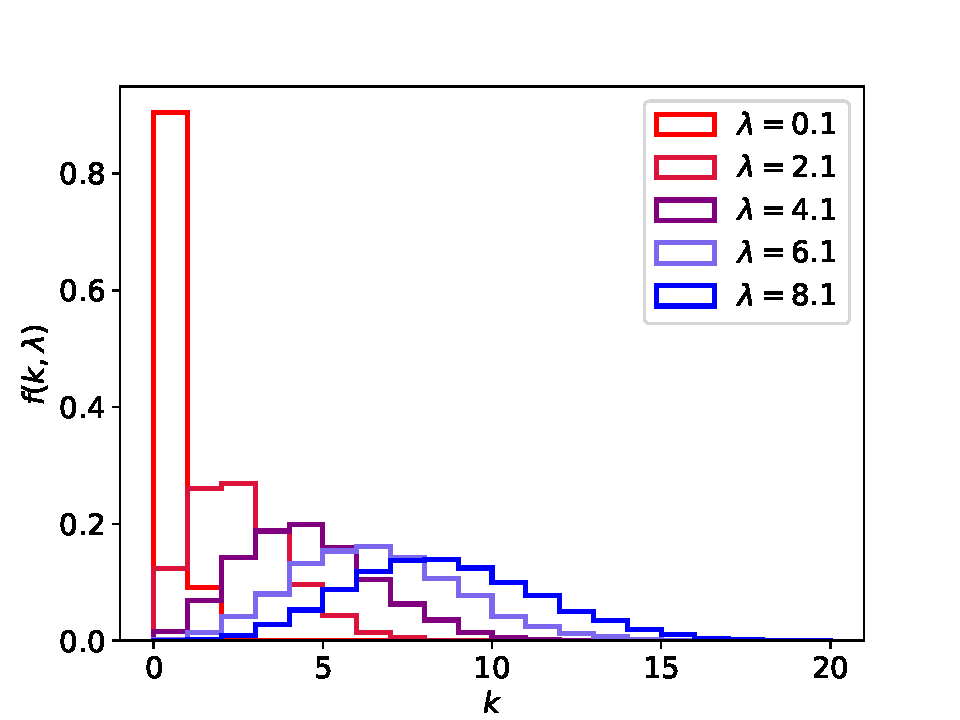
\includegraphics[width=0.8\textwidth]{figures/Probability/PoissonProbs.pdf}
    \caption{Poisson probability distribution $f(k;\lambda)$ for different values of the parameter $\lambda$. The distributions are produced by randomly generating 10,000 values (toys) of $k$ according to a Poisson distribution with parameter $k$, and creating the histogram of the results.}
    \label{fig:poissondistributions}
\end{figure}

\subsection{Continuous random variables and probability densities}

We can generalize probabilities (and distributions of probability) for events to probability distributions of \emph{continuous} random variables. A continuous random variable  is one whose possible values cover continuous intervals, for example $X\in\mathbb{R}$. In this case, we need to define something called a \emph{probability density function}. 

Suppose we measure the energy $E$ of cosmic ray particles. Due to the underlying quantum mechanics of interactions with the atmosphere, there will be a probability that the particle has a particular energy within some finite range $P(E \in (E+\delta E)$. As the energy is a continuous variable, we are free to choose $\delta E$ as small as we like. If there is a continuous function for all values of $E>0$ which represents the limit as $\delta E\rightarrow 0$, 
\begin{equation}
    f(E) = \mathrm{lim}_{\delta E\rightarrow 0}\frac{P(E \in (E+\delta E)}{\delta E}
\end{equation}
we call that function the \emph{probability density function} or p.d.f. The p.d.f must be normalised analogously to the discrete case such that, \begin{equation}
    \int_{\Omega} f(E)dE = 1, ~\mathrm{where} ~E\in\Omega.
\end{equation} 
Of course, as with the discrete case, we can measure multiple continuous quantities $\mathbf{X}$ in which case $d\mathbf{X}=dXdYdZ,...$ represents an infinitesimal volume. 

We can define two more distributions related to the probability density. The first is the \emph{cumulative distribution}, defined by the integral, 
\begin{equation}
    F(X) = \int_{X_{a}}^X f(X')dX' 
\end{equation}
where $X_a \leq X \leq X_b$, and $f(X)$ is the probability density distribution of $X$. Clearly then $F(X_a)=0$ and $F(X_b)=1$. We can interpret $F(X_{1})$ as the probability that $X\leq X_1$.  The cumulative distribution will be used later when we discuss $p$-values.

If the probability density function has more than one random variable, we can define a projection onto a fewer number of variables, which is called the \emph{marginal density}. For example, if we have a probability density $f(X,Y)$, the projection onto the $X$ variable is given by, 
\begin{equation}\label{eqn:marginal}
    g(X) = \int_{Y_{a}}^{Y_{b}} f(X,Y)dY 
\end{equation}
where $Y_a \leq Y \leq Y_b$.

We can also use Bayes theorem for continuous random variables. If $f(X,Y)$ is the probability density for two variable $X$ and $Y$, with marginal densities $g(X)$ and $h(Y)$, then Eqn.~\ref{eqn:bayesdiscrete} becomes, 
\begin{equation}
    q(Y|X) = \frac{p(X|Y)h(Y)}{g(X)},
\end{equation}
where $q(Y|X)$ and $p(X|Y)$ are the conditional probabilities defined through the relationship 
\begin{equation}
   f(X,Y)= p(X|Y)h(Y) = q(Y|X)g(X).
\end{equation}

\subsection{Moments of probability distributions}

Probability density distributions can be used to obtain useful information about a particular random variable, or functions of random variables. For example, the mean value of a random variable $X$ (or its \emph{expectation value} under $f(X)$ is given by, 
\begin{equation}\label{eqn:expectation}
    E[X] = \int_{\Omega} Xf(X)dX,
\end{equation}
where $E[\cdot]$ is the expectation operator. 
Similarly, any function of $X$, $g(X)$ has an expectation value $E[g]$ under $f(X)$ of,
\begin{equation}
    E[g] = \int_{\Omega} g(X)f(X)dX
\end{equation}
It should be obvious that the expectation is a \emph{linear} operator, since, 
\begin{equation}\label{eqn:linearexpectation}
    E[a\cdot g(X)+b\cdot h(Y)] = a\cdot E[g(X)]+b\cdot E[h(Y)]
\end{equation}
If the two variables $X$ and $Y$ are \emph{independent} then we also have that $ E[X\cdot Y] = E[X] E[Y]$.

The expectation value (mean) is often referred to as the \emph{first moment} of the distribution of $X$, but of course we can define higher moments too. For example, the expectation of the function $g(X)=(X-E[X])^{2}$ is called the \emph{variance} of $X$ under $f(X)$, 
\begin{equation}\label{eqn:variance}
    V(X) = E[(X-E[X])^{2}] = \int_{\Omega} (X-E[X])^2f(X)dX
\end{equation}
You will also have come across the term \emph{standard deviation}, $\sigma = \sqrt{V(X)}$. Note that the variance (or the standard deviation) is \emph{not} a linear operator. However, we do have the following properties, 
\begin{equation}
 V(X+a) = V(X) ~\mathrm{and}~ V(aX)=a^{2}V(X),
\end{equation}
when $a$ is a constant value. 

There are equivalents of the expectation and variance for discrete random variables too, $E[X]=\bar{X}=\sum_{\Omega}Xf(X)$, and $V(X)=\sum_\Omega (X-E[X])^2f(X)$.
\begin{tcolorbox}[colback = backblue]
\textbf{Example:} The expectation and variance of a discrete random variable $k$ distributed as a Poisson distribution can be calculated using the discrete versions of the formula given in Eqns.~\ref{eqn:expectation} and~\ref{eqn:variance}.
\begin{eqnarray}
E[k] & = & \sum_{k=0}^{\infty}ke^{-\lambda}\frac{\lambda^{k}}{k!}
      =  e^{-\lambda}\sum_{k=0}^{\infty}k\frac{\lambda^{k}}{k!}
      =  e^{-\lambda}\lambda e^{\lambda} \\
      & = & \lambda,
\end{eqnarray}
and,
\begin{eqnarray}
V(k) & = & \sum_{k=0}^{\infty}(k-\lambda)^2 e^{-\lambda}\frac{\lambda^{k}}{k!} \\
      & = & e^{-\lambda}\sum_{k=0}^{\infty}k^{2}\frac{\lambda^{k}}{k!}
      -2\lambda e^{-\lambda}\sum_{k=0}^{\infty}k\frac{\lambda^{k}}{k!}
      + \lambda^{2} e^{-\lambda}\sum_{k=0}^{\infty}\frac{\lambda^{k}}{k!} \\
      & = & \lambda+\lambda^{2} - 2\lambda^{2}+\lambda^{2} \\
      & = & \lambda
\end{eqnarray}
using the identities $(x^2+x)e^{x}=\sum_{k=0}^{\infty}k^{2}\frac{x^{k}}{k!}$, $xe^{x}=\sum_{k=0}^{\infty}k\frac{x^{k}}{k!}$, and $e^{x}=\sum_{k=0}^{\infty}\frac{x^{k}}{k!}$. So for $k\sim\mathrm{Poisson}(\lambda)$, we have $E[k]=V(k)=\lambda$.  
\end{tcolorbox}

Of course, there are other moments we can calculate which describe more properties of the probability distribution we're interested in. Specifically, 
\begin{equation}
    \mu_{n} = E[X^{n}] ~ \mathrm{is~the}~n^{\mathrm{th}}~\mathrm{algebraic~moment},
\end{equation}
and,
\begin{equation}
    \nu_{n} = E[(X-E[X])^{n}] ~ \mathrm{is~the}~n^{\mathrm{th}}~\mathrm{central~ moment}.
\end{equation}
Then we have that $E[X]=\mu_{1}$ and $V(X)=\nu_{2}$.
Often you'll see quantities which are constructed from these moments. For example, the \emph{skewness} of a probability distribution is given by, 
\begin{equation}
    \gamma = \frac{\nu_{3}}{(\nu_2)^{3/2}},
\end{equation}
which describes an asymmetry in the distribution. 
We can also determine moments of multidimensional distributions too. For example for a probability distribution $f(X,Y)$, the algebraic moment of order $m$ in $X$ and $n$ in $Y$ is $\mu_{mn}=E[X^{m}Y^{n}]$. The most common moment you'll come across is the \emph{co-variance}, which for an $M$ dimensional probability distribution $f(\mathbf{X})$, is the central moment of order 1 in two variables $X_{i}, X_{j}$ and order 0 for the remaining $M-2$ variables, 
\begin{equation}
    \mathrm{covariance}(X_{i},X_{j}) = \nu^{ij}_{1,1} = E[(X_{i}-E[X_{i}])(X_{j}-E[X_{j}])], 
\end{equation}
and the \emph{correlation coefficient} is given by 
\begin{equation}
    \mathrm{correlation}(X_{i},X_{j}) = \rho(X_{i},X_{j}) = \frac{\nu^{ij}_{1,1}}{\sqrt{v^{i}_{2}v^{j}_{2}}} , 
\end{equation}
where $v^{i}_{2}$, and $v^{j}_{2}$ are the variance of $X_{i}$ and $X_{j}$ respectively. The correlation coefficient will be $-1\leq \rho \leq 1$. 
Two variables $X$, $Y$ which are independent under $f(X,Y)$ will have a correlation coefficient of 0. The reverse is however not necessarily true so you should remember that \emph{independence} is a stronger statement than \emph{uncorrelated} (see problems for an example).  

\subsection{Compositions of probability distributions}

Compositions of random variables can be used to determine the distributions of derived quantities in HEP. We haven't covered what we mean by a ``measurement'' yet but you'll know that any measurement of a physical quantity is meaningless without an associated  ``uncertainty''. Actually, uncertainty in the sense we need for HEP won't be covered until the last sections of these lectures. However, you are probably aware of the concept at least in relation to the variance of a random variable. Often you'll have come across the idea of uncertainty being associated to the standard deviation -- $\sigma_{X} = \sqrt{V(X)}$. Quite correctly, if $X$ is a measured quantity, more often than not, it will be a random variable and we'll see that the standard deviation of this variable can be a pretty good approximation to a more concrete definition of uncertainty. You'll also have come across the concept of propagating uncertainties for quantities built from random variables such as the sum of two random variables $X$, $Y$. We already know that $E[X+Y]=E[X]+E[Y]$ by the linearity of expectation, but for the variance, the formula you know is, 
\begin{equation}\label{eqn:quadraturesum}
    V(X+Y) = V(X)+V(Y). 
\end{equation}
We'll see where this comes from. 

Suppose $X\sim f(X)$ and $Y\sim g(Y)$ are two independent random variables and $U=X+Y$. What is the probability distribution $p(U)$ of $U$?. First, we change variables to, \begin{equation}
    U = X+Y, ~V = X. 
\end{equation}
The probability distribution $h(U,V)$ is defined by, 
\begin{equation}
    h(U,V)dUdV = f(X)g(Y)dXdY,
\end{equation}
since the probability (not necessarily the density however) must be invariant under a change of variables.  for a change of variables, the infinitesimal volume $dXdY$ changes as, 
\begin{equation}
    dXdY =  \left|\mathrm{det} \begin{bmatrix} 
    \frac{\partial U}{\partial X} & \frac{\partial U}{\partial Y}\\
    \frac{\partial V}{\partial X} & \frac{\partial V}{\partial Y}
   \end{bmatrix}\right| ^{-1} dUdV=  dUdV
\end{equation}
then we have 
\begin{equation}
    h(U,V)dUdV = f(V)g(U-V)dUdV ~\implies h(U,V) = f(V)g(U-V).
\end{equation}
Recall that to obtain the marginal density $p(U)$, we integrate over $V$ (see Eqn.~\ref{eqn:marginal}) to obtain, 
\begin{equation}\label{eqn:sumsofrandoms}
    p(U) = \int_{-\infty}^{+\infty}h(U,V)dV =  \int_{-\infty}^{+\infty}f(U)g(U-V)dV.
\end{equation}
Note that we have relied on the fact that the change of variables $X,Y\rightarrow U,V$ is a \emph{bijection} (1 to 1 mapping). If it were not the case, then we could split the integral into segments over which each transformation is a bijection. 

\begin{tcolorbox}[colback=backblue]
\textbf{Example:} In the case that $X~\sim\phi(X;\mu_{X},\sigma_{X})$ and $Y~\sim\phi(Y;\mu_{Y},\sigma_{Y})$, where 
\begin{equation}\label{eqn:gaussian}
    \phi(x;\mu,\sigma) = \dfrac{1}{\sigma\sqrt{2\pi}} e^{-\dfrac{(x-\mu)^2}{2\sigma^{2}}}
\end{equation}
is the \emph{Gaussian} (or normal) distribution, we can find the probability distribution of $U=X+Y$. Plugging $\phi(\cdot)$ into Eqn.~\ref{eqn:sumsofrandoms} we find, 
\begin{eqnarray}
    p(U) & = & \int_{-\infty}^{+\infty}\frac{1}{\sigma_{X}\sqrt{2\pi}} \mathrm{exp}\left[{-\frac{(V-\mu_{X})^2}{2\sigma_{X}^{2}}}\right]\dfrac{1}{\sigma_{Y}\sqrt{2\pi}} \mathrm{exp}\left[{-\frac{(U-V-\mu_{Y})^2}{2\sigma_{Y}^{2}}}\right]dV\\
    & = & \int_{-\infty}^{+\infty} 
    \frac{1}{\sqrt{2\pi}\sqrt{2\pi}\sigma_{X}\sigma_{Y}} 
    \mathrm{exp}\left[{-\frac{(V-\mu_{X})^2}{2\sigma_{X}^{2}}-\dfrac{(U-V-\mu_{Y})^2}{2\sigma_{Y}^{2}}}\right]dV\\
    & = &   \int_{-\infty}^{+\infty} 
    \frac{1}{\sqrt{2\pi}\sqrt{2\pi}\sigma_{X}\sigma_{Y}} 
    \mathrm{exp}\left[
    -\frac{\sigma_{Y}^{2}(V-\mu_{X})^2 +\sigma_{X}^{2}(U-V-\mu_{Y})^2} {2\sigma_{X}^{2} \sigma_{Y}^{2}}
    \right]dV\\
    & = &   \int_{-\infty}^{+\infty} 
    \frac{1}{\sqrt{2\pi}\sqrt{2\pi}\sigma_{X}\sigma_{Y}} 
    \mathrm{exp}\left[
    A 
    \right]dV\\
\end{eqnarray}    
Expanding the exponent,
\begin{eqnarray}
    A
    & = & \frac{-(\sigma_{X}^{2}+\sigma_{Y}^{2})V^{2}+2\left(\sigma_{X}^{2}(U-\mu_{Y})+\sigma_{Y}^{2}\mu_{X}\right)V -\sigma_{X}^{2}(U^{2}+\mu_{Y}^{2}-2U\mu_{Y})-\sigma_{Y}^{2}\mu_{X}^{2}}{2\sigma_{X}^{2} \sigma_{Y}^{2}}\\
    & = & \frac{-\sigma_{U}^{2}V^{2}+2\left(\sigma_{X}^{2}(U-\mu_{Y})+\sigma_{Y}^{2}\mu_{X}\right)V -\sigma_{X}^{2}(U^{2}+\mu_{Y}^{2}-2U\mu_{Y})-\sigma_{Y}^{2}\mu_{X}^{2}}{{2\sigma_{X}^{2} \sigma_{Y}^{2}}}\\
    & = & \frac{-V^{2}+2\left(\sigma_{X}^{2}(U-\mu_{Y})+\sigma_{Y}^{2}\mu_{X}\right)\frac{V}{\sigma_{U}^{2}} -\dfrac{\sigma_{X}^{2}}{\sigma_{U}^{2}}(U-\mu_{Y})^{2}-\frac{\sigma_{Y}^{2}\mu_{X}^{2}}{\sigma_{U}^{2}}}{2\left(\frac{\sigma_{X} \sigma_{Y}}{\sigma_{U}}\right)^{2}},
 \end{eqnarray}   
where we have defined $\sigma_{U}^{2}=\sigma_{X}^{2}+\sigma_{Y}^{2}$. Now we can complete the square for $V$, to get, 
\begin{eqnarray}
    A & = & \frac{ 
    -\left(V-\frac{\sigma_{X}^{2}(U-\mu_{Y})+\sigma_{Y}^{2}\mu_{X}}{\sigma_{U}^{2}}\right)^{2} +\left(\frac{\sigma_{X}^{2}(U-\mu_{Y})+\sigma_{Y}^{2}\mu_{X}}{\sigma_{U}^{2}}\right)^{2} 
    - \frac{\sigma_{X}^{2}(U-\mu_{Y})^{2}+\sigma_{Y}^{2}\mu_{X}^{2}}{\sigma_{U}^{2}}}
    {2\left(\frac{\sigma_{X} \sigma_{Y}}{\sigma_{U}}\right)^{2}}.
\end{eqnarray}
If we plug $A$ back into the exponent we get, 
\begin{eqnarray}
  \mathrm{exp[A]} & = & \mathrm{exp}\left[\frac{ \left(\frac{\sigma_{X}^{2}(U-\mu_{Y})+\sigma_{Y}^{2}\mu_{X}}{\sigma_{U}^{2}}\right)^{2} 
    - \frac{\sigma_{X}^{2}(U-\mu_{Y})^{2}+\sigma_{Y}^{2}\mu_{X}^{2}}{\sigma_{U}^{2}}}
    {2\left(\frac{\sigma_{X} \sigma_{Y}}{\sigma_{U}}\right)^{2}} \right] \times \\ 
    & & 
    \mathrm{exp}\left[\frac{ 
    -\left(V-\frac{\sigma_{X}^{2}(U-\mu_{Y})+\sigma_{Y}^{2}\mu_{X}}{\sigma_{U}^{2}}\right)^{2}}{2\left(\frac{\sigma_{X} \sigma_{Y}}{\sigma_{U}}\right)^{2}}\right]
\end{eqnarray}
The first exponential is constant in $V$, so it can come outside of the integral. Furthermore, for the normalisation term, we have, 
\begin{eqnarray}
\frac{1}{\sqrt{2\pi}\sqrt{2\pi}\sigma_{X}\sigma_{Y}} & = & \frac{1}{\sqrt{2\pi}\sigma_{U}} \frac{\sigma_{U}}{\sqrt{2\pi}\sigma_{X}\sigma_{Y}}
\end{eqnarray}
so then, 
\begin{eqnarray}
p(U) & = & \frac{1}{\sqrt{2\pi}\sigma_{U}}\mathrm{exp}\left[\frac{ \left(\frac{\sigma_{X}^{2}(U-\mu_{Y})+\sigma_{Y}^{2}\mu_{X}}{\sigma_{U}^{2}}\right)^{2} 
    - \frac{\sigma_{X}^{2}(U-\mu_{Y})^{2}+\sigma_{Y}^{2}\mu_{X}^{2}}{\sigma_{U}^{2}}}
    {2\left(\frac{\sigma_{X} \sigma_{Y}}{\sigma_{U}}\right)^{2}} \right] \times \\ 
    & & 
    \int_{-\infty}^{+\infty}\dfrac{1}{\sqrt{2\pi}\frac{\sigma_{X}{\sigma_{Y}}}{\sigma_{U}}}
    \mathrm{exp}\left[\frac{ 
    -\left(V-\frac{\sigma_{X}^{2}(U-\mu_{Y})+\sigma_{Y}^{2}\mu_{X}}{\sigma_{U}^{2}}\right)^{2}}{2\left(\frac{\sigma_{X} \sigma_{Y}}{\sigma_{U}}\right)^{2}}\right]dV.
\end{eqnarray}
\end{tcolorbox}
\begin{tcolorbox}[colback=backblue]
The term inside the integral is just a Gaussian distribution in $V$ (with $\sigma=\frac{\sigma_{X}\sigma_{Y}}{\sigma_{U}}$), so the integral just yields 1. Therefore, 
\begin{eqnarray}
p(U) & = & \frac{1}{\sqrt{2\pi}\sigma_{U}}\mathrm{exp}\left[\frac{ \left(\frac{\sigma_{X}^{2}(U-\mu_{Y})+\sigma_{Y}^{2}\mu_{X}}{\sigma_{U}^{2}}\right)^{2} 
    - \frac{\sigma_{X}^{2}(U-\mu_{Y})^{2}+\sigma_{Y}^{2}\mu_{X}^{2}}{\sigma_{U}^{2}}}
    {2\left(\frac{\sigma_{X} \sigma_{Y}}{\sigma_{U}}\right)^{2}} \right]\\
    & = & 
    \frac{1}{\sqrt{2\pi}\sigma_{U}}\mathrm{exp}\left[\frac{ \left({\sigma_{X}^{2}(U-\mu_{Y})+\sigma_{Y}^{2}\mu_{X}}\right)^{2} 
    - \sigma_{U}^{2}\left({\sigma_{X}^{2}(U-\mu_{Y})^{2}+\sigma_{Y}^{2}\mu_{X}^{2}}\right)}
    {2\sigma_{U}^{2}\left({\sigma_{X} \sigma_{Y}}\right)^{2}} \right]\\
    & = & 
    \frac{1}{\sqrt{2\pi}\sigma_{U}}\mathrm{exp}\left[\frac{ \left({\sigma_{X}^{2}(U-\mu_{Y})+\sigma_{Y}^{2}\mu_{X}}\right)^{2} 
    - \sigma_{U}^{2}\left({\sigma_{X}^{2}(U-\mu_{Y})^{2}+\sigma_{Y}^{2}\mu_{X}^{2}}\right)}
    {2\sigma_{U}^{2}\left({\sigma_{X} \sigma_{Y}}\right)^{2}} \right]\\
    & = & 
    \frac{1}{\sqrt{2\pi}\sigma_{U}}\mathrm{exp}\left[-\frac{ (U-(\mu_{X}+\mu_{Y})^{2})(\sigma_{X}\sigma_{Y})^{2}}
    {2\sigma_{U}^{2}\left({\sigma_{X} \sigma_{Y}}\right)^{2}} \right]\\
     & = & 
    \frac{1}{\sqrt{2\pi}\sigma_{U}}\mathrm{exp}\left[-\frac{ (U-(\mu_{X}+\mu_{Y})^{2})}
    {2\sigma_{U}^{2}} \right],
\end{eqnarray}
which is a Gaussian distribution with $\mu_{U}=\mu_{X}+\mu_{Y}$, and $\sigma_{U}^{2}=\sigma_{X}^{2}+\sigma_{Y}^{2}$ or $V(U)=V(X)+V(Y)$.
\end{tcolorbox}

So there we have shown that the sum of two random normal variables yields another normally distributed random variable and we've verified Eqn.~\ref{eqn:quadraturesum}! We can check that our calculation is correct in an example. The following \textsf{Python3} code will generate toys from two Gaussian distributions $X\sim\phi(X;10,1)$, $Y\sim\phi(Y;-6,0.5)$ using the \textsf{numpy.random.normal} function. The generated values of $X$ and $Y$ are summed, and those values are filled into a histogram. We should be able to see that this distribution looks like another Gaussian distribution with $\mu=-6+10=4$ and $\sigma=\sqrt{0.5^2+1^2}=1.1$. 

\begin{lstlisting}[style = Python]
import numpy
import matplotlib.pyplot as plt

def gaus(x,mu,sigma):
 A = (1./(sigma*(2*numpy.math.pi)**0.5))
 B = numpy.math.exp(-(x-mu)*(x-mu)/(2*sigma*sigma))
 return A*B
 
muX, sigmaX = 10., 1.
muY, sigmaY = -6., 0.5

# generate toy values from the two Gaussian distributions and sum
toys_X = numpy.random.normal(muX,sigmaX,1000)
toys_Y = numpy.random.normal(muY,sigmaY,1000)
toys_U = toys_X+toys_Y

# plot the toys and compare to the expected Gaussian distributions
x = numpy.arange(-10,20,0.1)

plt.hist(toys_X,100,(-10,20),density=True,color='green')
plt.hist(toys_Y,100,(-10,20),density=True,color='red')
plt.hist(toys_U,100,(-10,20),density=True,color='cyan')

# according to our calculation for the sum of two Gaussian variables
mu    = muX + muY
sigma = ((sigmaX)**2 + (sigmaY)**2)**0.5

plt.plot(x,[gaus(xx,mu,sigma) for xx in x],color='black')
print("mu=%.1f, sigma=%.1f"%(mu,sigma))

plt.xlabel("$U$")
plt.ylabel("$\\phi(U)$")
plt.show()
\end{lstlisting}

The output of the code is shown in Fig.~\ref{fig:gaussiansum}. 
\begin{figure}[hbt!]
    \centering
    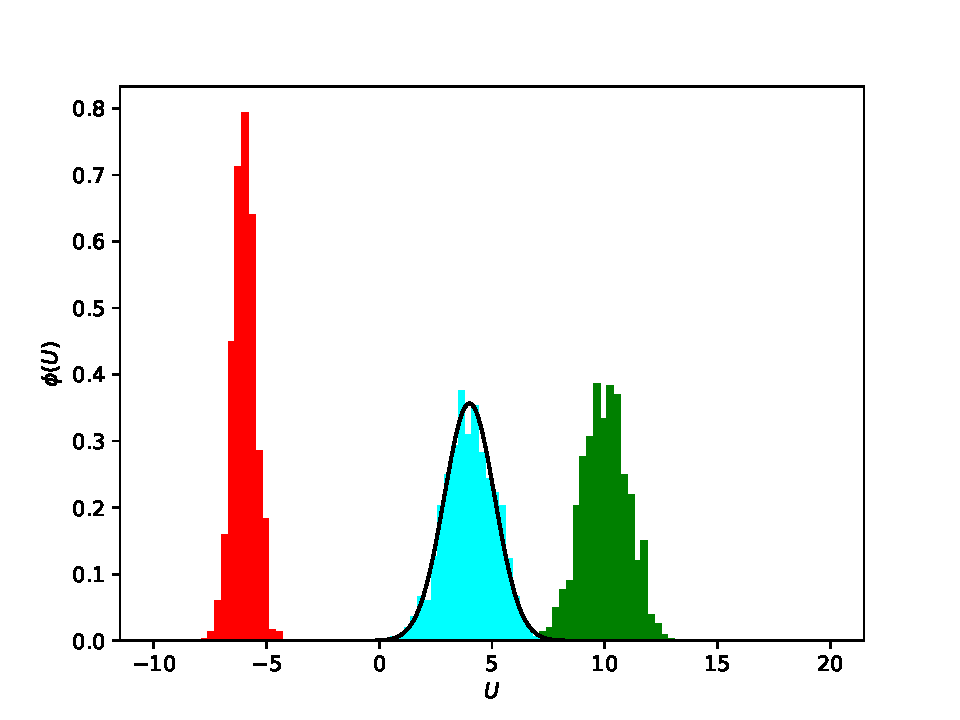
\includegraphics[width=0.8\textwidth]{figures/Probability/GaussianSum.pdf}
    \caption{Distribution of toys generated from a Gaussian with $\mu=-6,~\sigma=0.5$ (red histogram) and $\mu=-10,~\sigma=1$ (green histogram). The cyan histogram shows the distrubtion of the sum of the toys, and the black line shows the Gaussian distribution with $\mu=-6+10=4$ and $\sigma=\sqrt{0.5^2+1^2}=1.1$. }
    \label{fig:gaussiansum}
\end{figure}
Be warned however, that compositions of even Gaussian random variables doesn't always result in something Gaussian. For example, if $X\sim \phi(X;0,1)$ and $Y\sim \phi(Y;0,1)$ and $U=\frac{X}{Y}$, then (as you'll show in one of the problems) $p(U)$ is a Cauchy distribution, 
\begin{equation}
    p(U) = \dfrac{1}{\pi(1+U^{2})},
\end{equation}
which has no mean value and infinite variance!. In this case, the usual error propagation formula can be quite misleading. 
 

\section{The convergence law of large numbers}

You are certainly aware of the concept of \emph{convergence}. We used it already to demonstrate how the Poisson distribution arises from the binomial distribution when the probability of success is very small. In statistics, there are different kinds of convergence so we need to be careful to specify the sense in which something converges to another. The two most common senses in statistics are \emph{convergence in distribution} and \emph{convergence in probability}. First, we will define these two senses, without much discussion as to their application. This is because in the end, as particle physicists, the main result we care about is the \emph{central limit theorem}, which turns out to be extremely powerful for testing hypotheses and measuring physical properties -- i.e for the main job of a particle physicist. 
\paragraph{Convergence in distribution:}
Consider a sequence of random variables $\{X_{1},X_{2},...,X_{n}\}$ with cumulative distribution functions $\{F(X_{1}),F(X_2),...,F(X_{n})\}$. The sequence $X_{n}$ converges in distribution as $n\rightarrow \infty$ to $X$, with cumulative distribution $F$ if for every point where $F(X)$ is continuous, 
\begin{equation}
    \mathrm{lim}_{n\rightarrow \infty}F_{n}(X) = F(X).
\end{equation}
\paragraph{Convergence in probability:}
We say that the sequence of random variables $\{X_{1},X_{2},...,X_{n}\}$, \emph{converges in probability} to $X$ if for any $\epsilon > 0$ and $\delta>0$, there exists a value of $N$ such that, 
\begin{equation}
    P(|X_{n}-X|>\epsilon) < \delta, 
\end{equation}
for all $n\geq N$. This definition of convergence is stronger than convergence in distribution since nothing about the distance between $X$ and $X_{n}$ is implied in the other definition. Convergence in probability implies convergence in distribution. 

The most important application of convergence is in the law of large numbers, which concerns the convergence of the sample mean. Let $\{X_{1},...X_{N}\}$ be a sequence of \emph{independent} random variables, each having the same mean $\mu_{1}$ and variances $\nu^{i}_{2}$. We determine the \emph{sample mean}, $\bar{X}$ as, 
\begin{equation}
    \bar{X} = \frac{1}{N}\sum_{i=1}^{N}X_{i}.
\end{equation}
Note that this is not the same as $\mu_{1}$ since this refers to the expectation value of $X_i$ under their probability distributions. If $\mu_{1}$ exists, then if either, 
\begin{eqnarray}
  \mathrm{lim}_{N\rightarrow \infty} \left[\frac{1}{N^{2}}\sum_{i=1}^{N}\nu^{i}_{2} \right] = 0 & \mathrm{\textbf{or}} & \mathrm{lim}_{N\rightarrow \infty}\left[\sum_{i=1}^{N}\frac{\nu^{i}_{2}}{i^{2}} \right] \mathrm{~is~finite}, 
\end{eqnarray}
then $\bar{X}$ converges in probability to $\mu_{1}$. 

\subsection{The central limit theorem}
So far we have talked separately convergence of sequences of  distributions and the convergence of the sample mean of independent random variables. The \emph{central limit theorem} (CLT) states how the sum of independent random variables (for example as in sample means) is \emph{distributed} in the limit of large $N$. 
Suppose we have a sequence of independent random variables $X_{i}$, each from a distribution with mean $\mu_{1}^{i}$ and variance $\nu_{2}^{i}$. Now let, 
\begin{equation}\label{eqn:clt}
   T_{N}= \dfrac{\bar{X}N - \sum_{i=1}^{N} \mu_{1}^{i}}{\sqrt{\sum_{i=1}^{N}\nu^{i}_{2}}}.
\end{equation}
Then for $T=\lim_{N\rightarrow \infty}T_{N}$, we have that $T\sim \phi(T;0,1)$ -- meaning that the limit $T$ is distributed as a standard normal distribution (a Gaussian with a width of 1 and a mean of 0) -- $T_{N}$ converges in distribution to a standard normal distribution. 

We could attempt to demonstrate this by explicitly writing out the probability for the sum of the random variables to be contained in some small interval - but remember how long and tedious that was with just summing two normal distributed variables! Instead, we can rely on the \emph{Paul Levy theorem} to do the heavy lifting. First, we define the \emph{characteristic function} $\varphi_{X}(t)$ of a probability distribution function $f(X)$  by, 
\begin{equation}
    \varphi_{X}(t)  = E\left[ e^{itX}\right] = \int_{-\infty}^{\infty} e^{itX}f(X)dX.
\end{equation}
The characteristic function completely determines the probability distribution of the random variable - i.e if we know $\varphi_{X}(t)$, then we know $f(X)$ too. The characteristic function has useful properties, for example, if $X$ and $Y$ are independent random variables, with characteristic functions  $\varphi_{X}(t)$ and $\varphi_{Y}(t)$, then the characteristic function of the sum $X+Y$ is $ \varphi_{X+Y}(t) =  \varphi_{X}(t) \cdot \varphi_{Y}(t) $. Furthermore, the characteristic function of the sum of independent variables is the product of the individual characteristic functions of the variables, i.e, 
\begin{equation}\label{eqn:prodcharacteristic}
    \varphi_{X_1+...+X_{N}}(t)  = \prod_{i=1}^{N}\varphi_{X_{i}}(t).
\end{equation}
We can use this to demonstrate the central limit theorem in the case of a sum of independent and identically distributed random variables. 

\begin{tcolorbox}[colback=backblue]
\textbf{Example:} Let $\{X_{1},...,X_{N}\}$ be independent and identically distributed random variables with $E(X)=0$ and $V(X)=\nu\in\mathbb{R}$. Then, 
\begin{equation}
    T_{N} = \frac{X_{1}+...+X_{N}}{\sqrt{\nu N}} = \sum_{i=1}^{N}\frac{Y_{i}}{\sqrt{N}}.
\end{equation}
where $Y_{i}$ = $X_{i}/\sqrt{\nu}$. We can say that the characteristic function of $T_{N}$ is given by, 
\begin{equation}\label{eqn:chartn}
    \varphi_{T_{N}} = \varphi_{Y_{1}}\left(\frac{t}{\sqrt{N}}\right)\cdot \varphi_{Y_{2}}\left(\frac{t}{\sqrt{N}}\right)\cdot...\cdot\varphi_{Y_{N}}\left(\frac{t}{\sqrt{N}}\right) = \left(\phi_{Y_{1}}\left(\frac{t}{\sqrt{N}}\right)\right)^N
\end{equation}
from Eqn.~\ref{eqn:prodcharacteristic} and the linearity property of the expectation. Recall that the characteristic function is given by the expectation so, 
\begin{equation}
    \varphi_{Y_{1}}\left(\frac{t}{\sqrt{N}}\right) = E\left[e^{i\dfrac{t}{\sqrt{N}}Y_{1}}\right] = E\left[ \sum_{r=0}^{\infty}\dfrac{\left(i\dfrac{t}{\sqrt{N}}Y_1\right)^{r}}{r!} \right] = \sum_{r=0}^{\infty}\dfrac{\left(i\dfrac{t}{\sqrt{N}}\right)^{r}}{r!}E\left[Y_1^{r}\right]
\end{equation}
where we have Taylor expanded the exponential. Now, we know that the mean of $Y_{1}$ is 0 (since also $\mu=0$) and the variance of $Y_{1}$ will be the same as the variance of $X_{1}$ divided by itself, hence $E\left[Y^{2}\right] = V(Y_1)=1$. So we have, 
\begin{equation}
    \varphi_{Y_{1}}\left(\frac{t}{\sqrt{N}}\right) = 1 - \dfrac{t^{2}}{2N} + \mathcal{O}\left(\frac{t^{3}}{N^{\frac{3}{2}}} \right).
\end{equation}
Substituting this back into Eqn.~\ref{eqn:chartn}, we have that as $N\rightarrow \infty$, $\varphi_{T_{N}}\rightarrow e^{-\frac{1}{2}t^{2}}$, which is the characteristic function of a standard normal distribution. From the Paul Levy theorem, this means that the limit of $T_N$, $T$, is distributed as a standard normal distribution -- $T\sim \phi(T;0,1)$. 
\end{tcolorbox}

Let's have a look at the CLT in action with a simulation. In the code below, the idea is to simulate a Galton Machine, in which a counter is dropped through layers of pins which force the counter to go left or right. Figure~\ref{fig:galton} shows the setup with 5 layers of pins. In the code, for each layer, we'll randomly choose left or right for the counter direction and make a histogram of the position for many counters. 

\begin{lstlisting}[style = Python]
import numpy
import matplotlib.pyplot as plt

# 50-50 probability to go left or right
def galton_step(x):
 r = numpy.random.uniform(0,1)
 if r < 0.5: return x-1
 else: return x+1

n_layers = 100
n_trials = 10000

finish=[]

for i in range(n_trials):
  start=0
  for j in range(n_layers): start = galton_step(start)
  finish.append(start)

# Histogram should have integer values as bin centres so shift by 0.5
plt.hist(finish,2*n_layers+1,(-1*n_layers-0.5,n_layers+0.5),\
    density=True,color='green')
plt.xlabel("position")
plt.ylabel("number of counters")
plt.title("N layers = %d, N trials = %d"%(n_layers, n_trials))
plt.show()
\end{lstlisting}
For different numbers of layers, we can see how the Gaussian distribution shape builds up as the number of layers increases in Figure~\ref{fig:simgalton}. The final position is the sum of random integer variables, each of which has a distribution that is uniform between -1 and +1. This is the CLT in action! We can actually see two laws of large numbers at play - the CLT is what guarantees the converge in distribution to a Gaussian shape, while the law of large numbers is behind the fact that the mean value for each bin converges to the probability density as we increase the number of trials. The latter is convergence in probability and is what we rely on when using Monte Carlo (MC) simulations in particle physics event generators. This method of generating a Gaussian distribution is of course very inefficient -- our modern day MC generators use much more sophisticated methods to generate probability (density) distribution functions for particle event simulations.  
\begin{figure}[hbt!]
    \centering
    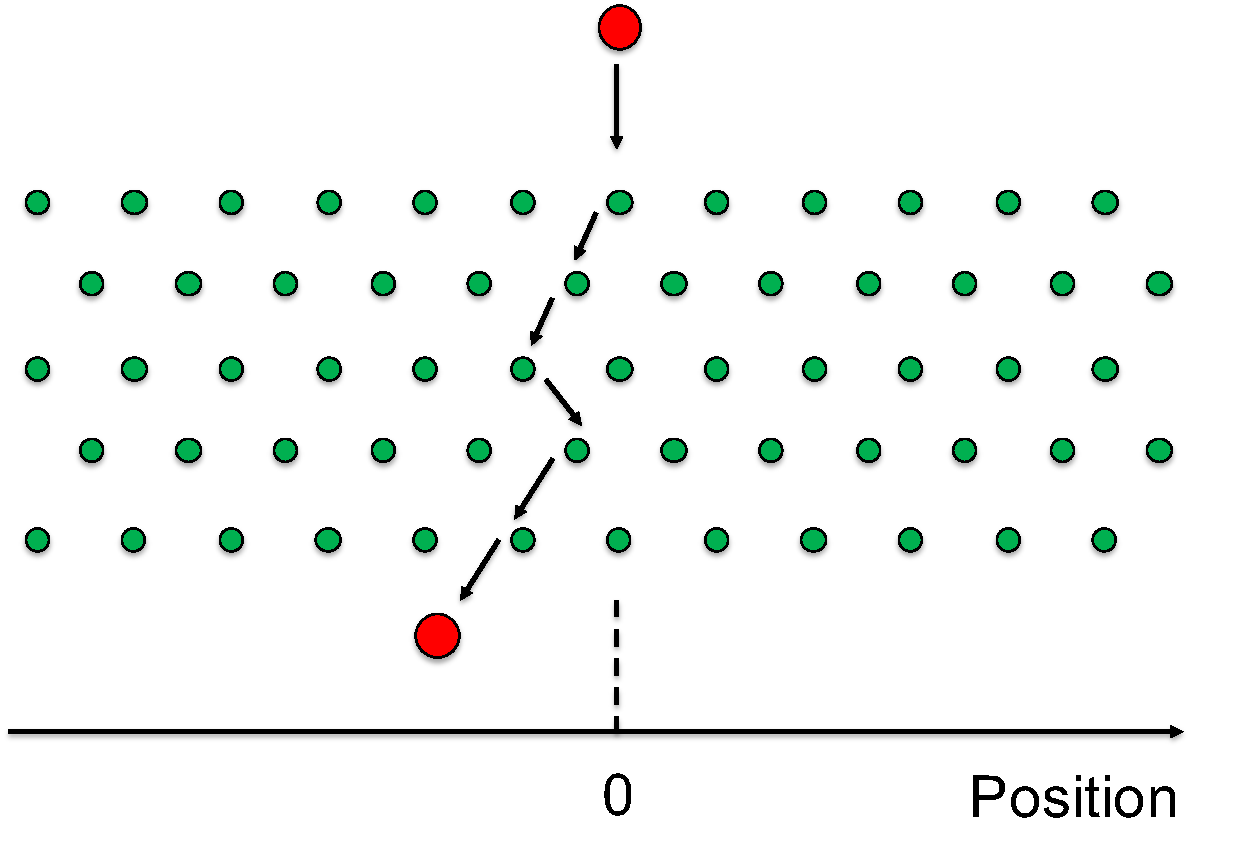
\includegraphics[width=0.6\textwidth]{figures/Probability/galton_image.pdf}
    \caption{The Galton machine: The idea is to drop the red counter down and let it work its way to the bottom. Each green pin will knock the counter left (-1 to its position) or right (+1 to its position) with an equal probability for each. At the end we'll count how many counters are at each position.}
    \label{fig:galton}
\end{figure}

\begin{figure}[hbt!]
    \centering
    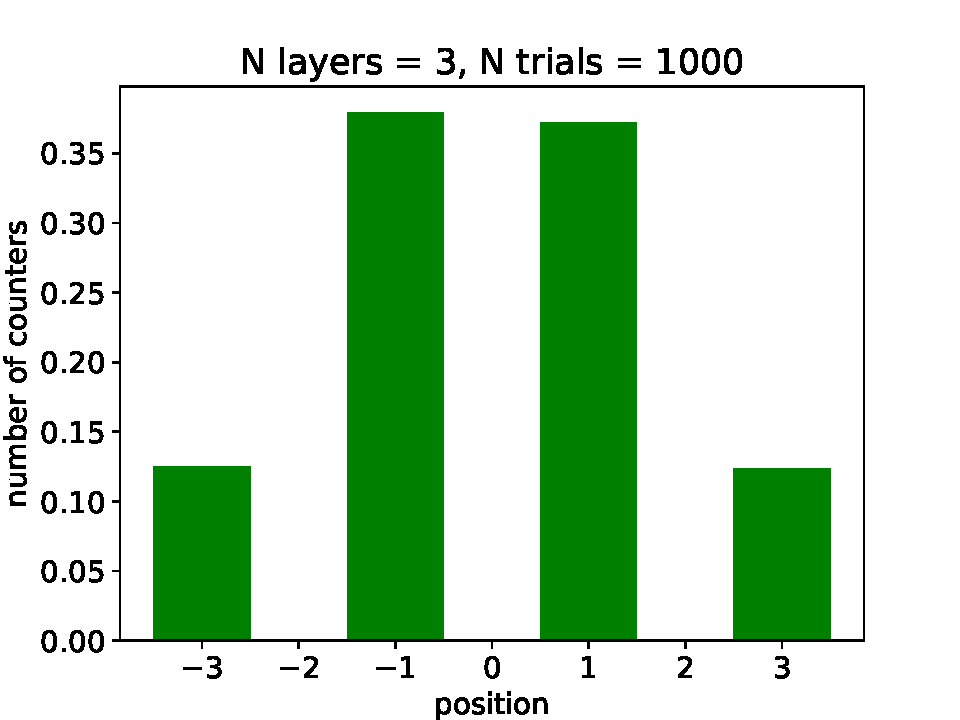
\includegraphics[width=0.32\textwidth]{figures/Probability/layers3.pdf}
    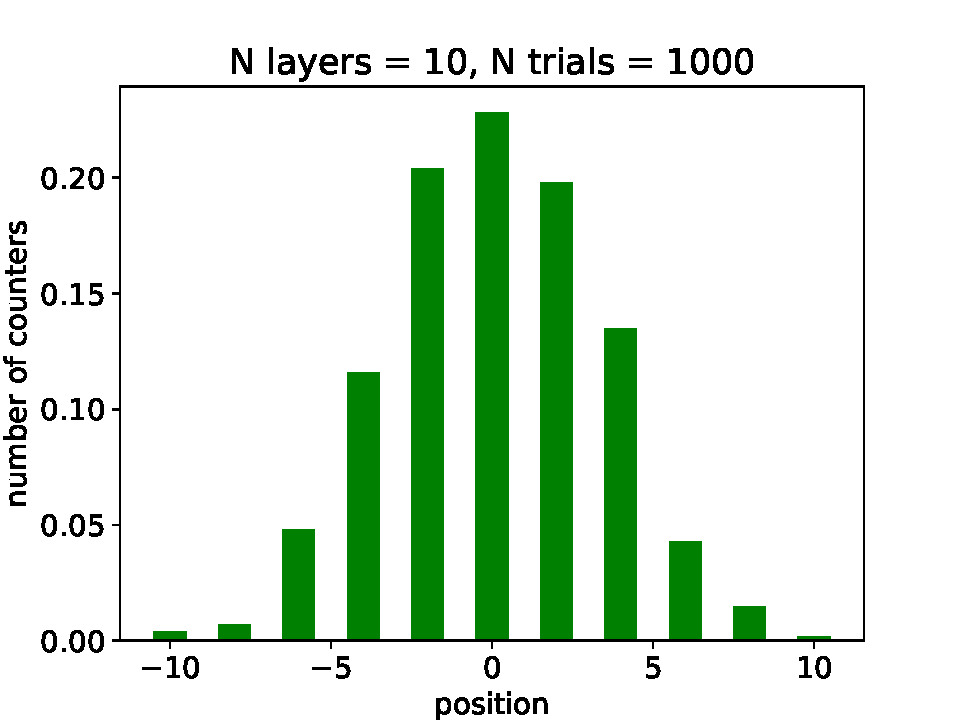
\includegraphics[width=0.32\textwidth]{figures/Probability/layers10.pdf}
    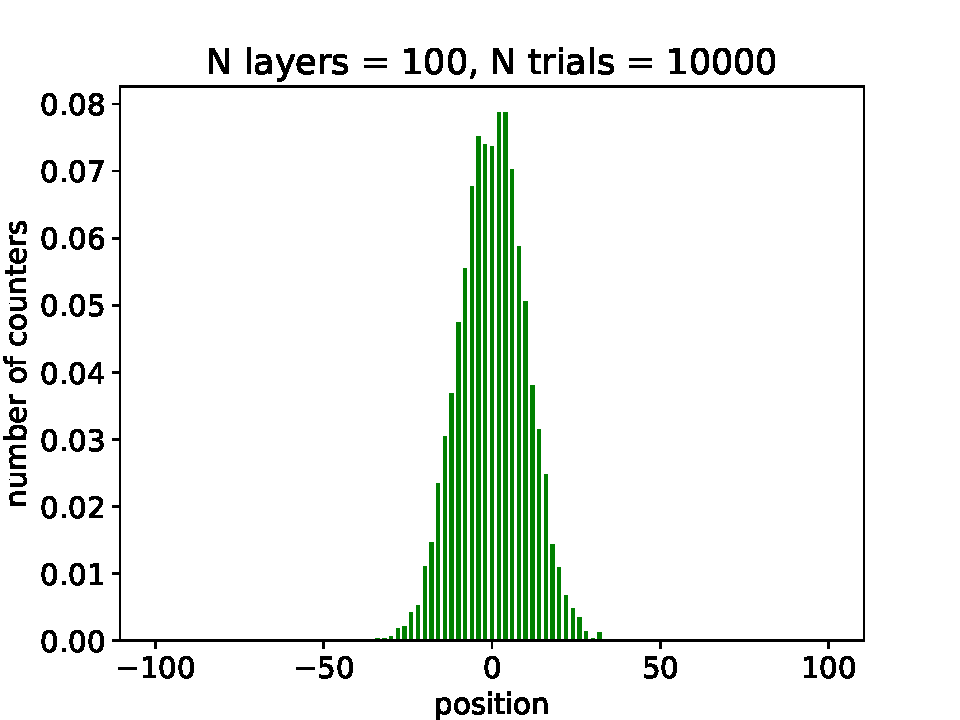
\includegraphics[width=0.32\textwidth]{figures/Probability/layers100.pdf}
    \caption{Galton machine simulation for 3, 10 and 100 layers. As the number of layers increases, we need more trials (counters) to fill in the possible positions but also we start to see the Gaussian distribution appear.}
    \label{fig:simgalton}
\end{figure}
\section{Hypothesis testing}\label{sec:hypotest}
So far, we have only discussed the concept of \emph{probability} and probability distributions. While this is a very important topic, we haven't yet touched on the main tool-set for a particle physicist.  The concept of \emph{testing hypotheses} is of course at the heart of experimental science -- confronting a scientific hypothesis with data is the way we progress science after all.  Hypothesis testing is part of a whole branch in statistics called \emph{decision theory}. In these lectures, we won't have time to go into details about decision theory -- You can refer to James' book for a good discussion on decision theory, including the difference in approaches between Bayesians and frequentists. Instead it's enough to know that decision theory is concerned with the concept of reaching a decision, on the basis of experimental data, which will minimise the potential loss resulting from making the wrong decision -- should we adjust the trigger settings to improve our selection efficiency? Should we build another particle collider? Should we go outside without that umbrella? Our focus here will be on the tools used to make these decisions (rather than the decision making itself). This is where the concept of hypothesis testing enters.

In particle physics, we often deal with the case that one or more of our hypotheses involve some unknown parameter. We refer to these as \emph{composite hypotheses}. If there are no unknowns however, the hypothesis is completely specified and we call this a \emph{simple hypothesis}. A composite hypothesis can obviously be thought of as an ensemble of simple hypothesis. For now, lets stick to simple hypotheses. 
 
 Suppose that we have to choose between two hypotheses labelled $H_{0}$ and $H_{1}$, based on some experimental observations. We typically distinguish the two as $H_{0}:=$ \emph{the null hypothesis}, and $H_{1}:=$ \emph{the alternate hypothesis}. This is just a convention and we'll see that depending on the test, the null and alternate can switch places.  Let $X$ be a function of the experimental observations which is supposed to summarize the observations -- this is known as a \emph{test statistic}. Choosing the best test statistic to summarize your experiment can be difficult, especially if the setup is complicated, but we'll see that there is a key result to guide us in this choice. First we need to establish a concept which you may be familiar and that is \emph{errors} of type-I and type-II. 
 
 \subsection{Type-I and type-II errors}
 Again, let's suppose we have a null hypothesis ($H_{0}$) and an alternate ($H_{1}$) Suppose then that we have our chosen test statistic $X\in \mathcal{W}$. We divide this region $\mathcal{W}$ into a \emph{critical region} ${w}$ and a \emph{region of acceptance} $\mathcal{W}-{w})$. Observations of $X$ falling into $w$ would lead us to believe that our null hypothesis is not true. Defining a \emph{test} of $H_{0}$ , given we've decided on our test statistic, then becomes choosing a critical region $w$. 
 
In practise, we often tune the critical region so as to obtain a particular probability (known as the \emph{size} of the test) $\alpha$ that $X$ falls into the critical region when $H_0$ is true (we usually say ``under $H_0$''), 
\begin{equation}\label{eqn:testsize}
     P(X\in w|H_{0})=\alpha.
\end{equation}
This is also referred to as the \emph{size} of the test. 
You can see then that $\alpha$ is exactly the probability to \emph{reject} the null hypothesis if the null hypothesis is \emph{true} - we call this a \emph{type-I error}. Thus, when defining a test, we have to accept that sometimes we will make this error. You'll often find that the level at which we set $\alpha$ strongly depends on what $H_0$ is. If for example, $H_0$ is a SUSY model with a particular mass scale, we might accept $\alpha=0.05$ as a reasonable error. However, if $H_0$ is the standard model of particle physics, we'd certainly want to choose a much smaller number. 

Of course, we also want to know how useful a test is at discriminating against the alternate hypothesis. This is known as the \emph{power of the test}, and is defined as the probability of $X$ falling into the critical region if $H_1$ is true (under $H_1$), 
\begin{equation}\label{eqn:power}
     P(X\in w|H_{1})=1-\beta.
\end{equation}
Clearly this is related to the probability that $X$ falls into the acceptance region via,
\begin{equation}
 P(X\in w|H_{1})=1-P(X\in \mathcal{W}-w|H_{1})=\beta.
\end{equation}
This is then the probability that we would \emph{accept} the null hypothesis when the alternative is true -- this is known as a \emph{type-II} error. Of course, we want to make sure this error is equally unlikely, hence the choice of a test will amount to maximising the power of the test $(1-\beta)$ for a fixed size of the test.  Figure~\ref{fig:htestregions} summarizes these two types of errors. 
\begin{figure}[hbt!]
    \centering
    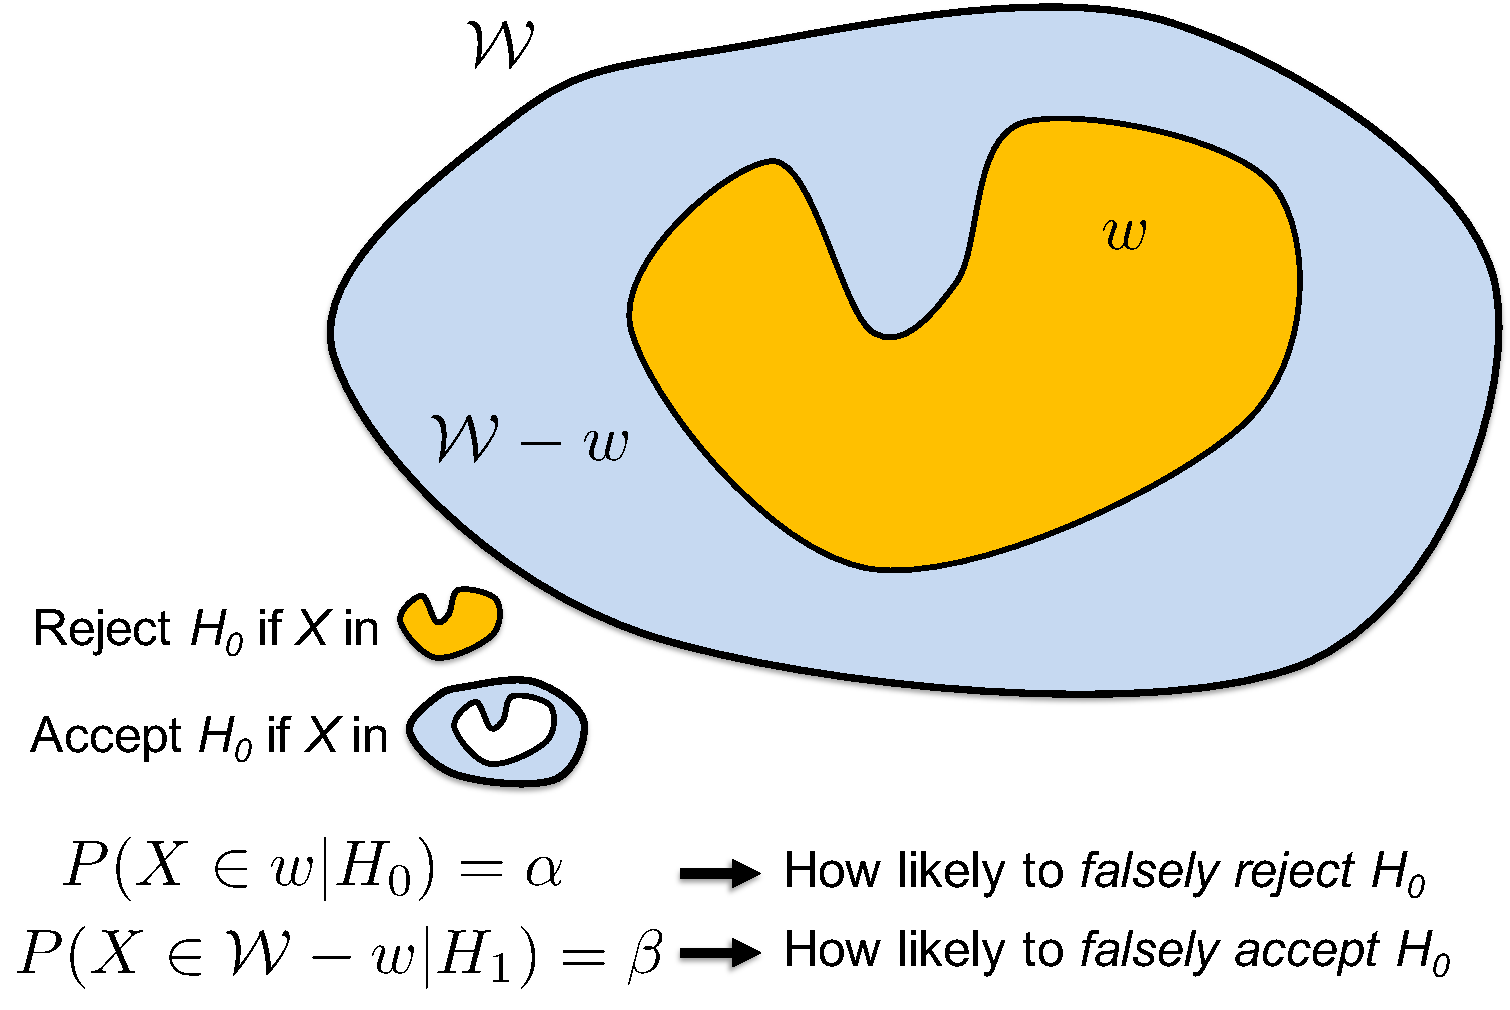
\includegraphics[width=0.6\textwidth]{figures/Hypotest/type12.pdf}
    \caption{Division of possibilities for the test statistic ($X$) into the yellow critical region $w$, and the blue region of acceptance $(\mathcal{W}-w)$. The probabilities that $X$ falls into the critical region, under the null hypothesis and alternate hypothesis are $\alpha$ and $(1-\beta)$, respectively.}
    \label{fig:htestregions}
\end{figure}
Some caution should be taken here. Remember we are dealing with two distinct simple hypotheses that cannot both simultaneously be true. Hence accepting one hypothesis means we are forced to reject the other (and vice versa). Particle physicists however don't usually talk about accepting hypotheses but rather rejecting them or not. This is because we rarely ever have a single test to establish that something is true, but we are often happy to use a single test to reject it - it's actually nearly always the same way with science, we tend to disprove theories  rather than prove them outright.

\begin{tcolorbox}[colback=backblue]
\textbf{Example:} Let's suppose we have a simple experimental setup that counts the number of charged particles, say electrons from a beam passing through a spark chamber. Say we can tune the beam to fire a fixed number of electrons at the chamber, and record the number of sparks $k$. When we ordered the detector, the manufacturer said it was 90\% efficient. So we set out to test our null hypothesis corresponding to $\epsilon=70\%$ hypothesis. Our test statistic will be $k$, and our critical region will correspond to values of $k\leq K$, where $K$ is the number satisfying, 
\begin{equation}
    \sum_{k=0}^{k=K} b(k;\epsilon,N),
\end{equation}
where $b(k;p,N)$ the our binomial probability distribution with success probability $\epsilon$ and $N$ trials. 

Suppose we run our experiment with 5000 electrons and observe 3420 sparks. Given this observation, we can think of Eqn.~\ref{eqn:testsize} as calculating the value of $\alpha$ where $K$ is our observation -- i.e instead of choosing $K$ such that $\alpha=0.05$, we  $K=83$ and compare the resulting value of $\alpha$ with 0.05. This is what is known as calculating a $p$-value (or tail probability) for a particular observation. We can calculate this numerically using a MC method - remember that convergence in probability requires a lot of MC. 

\begin{lstlisting}[style = Python]
import numpy as np
# parameters of the binomial probability distribution
N, eps=5000,0.70
# our observed number of sparks
K=3420

# generate MC pseudo observations
nMC=10000
random_k = np.random.binomial(N,eps,nMC)

# count the fraction of times we see a value of k
# less than or equal to K
pval = float(len([x for x in random_k if x<=K]))/nMC
print(pval)
\end{lstlisting}
We get a $p$-value of 0.0083.  This is smaller than 0.05 so based on this test we reject $H_0$. Of course we could have just calculated this $p$-value analytically but for more complicated test statistics, we will need to use MC methods.  
\end{tcolorbox}

In the example, we made our decision based on the $p$-value being smaller than 0.05, and we can check how often we would reject $H_0$, if it is true, based on this decision process. How often would we see a $p$-value smaller than 0.05? We can use MC to calculate it, but this time, we will use \textsf{binom} from the \textsf{scipy.stats} package (much faster). 
\clearpage
\begin{lstlisting}[style = Python]
import numpy as np
import matplotlib.pyplot as plt
# scipy has a lot of common pdfs for us to use
from scipy.stats import binom

# parameters of the binomial probability distribution
N, eps=5000,0.70

def calc_pval():
  # for a random observation K, we calculate the p-val
  # this time, just use in the handy scipy cdf
  K = np.random.binomial(N,eps)
  pval = binom.cdf(K,N,eps)
  return pval

nTests=10000
pvals = [calc_pval() for test in range(nTests)]
y,binEdges = np.histogram(pvals,bins=10)
bincenters = 0.5*(binEdges[1:]+binEdges[:-1])
menStd     = np.sqrt(y)
plt.bar(bincenters, y, width=0.025, yerr=menStd)
plt.xlabel("$p$-value")
plt.ylabel("Number of trials per bin")
plt.show()
\end{lstlisting}
This produces the plot shown in Figure~\ref{fig:p0dist}. You can see its flat. Actually this is not surprising since the distribution of the $p$-value under the null hypothesis is always flat\footnote{For a discrete test statistic its approximately flat but if our test statistic were continuous it really would be flat}! Immediately we can see then that by choosing to reject $H_0$ when the $p$-value is  exactly the probability that we would falsely reject $H_0$!

\begin{figure}
    \centering
    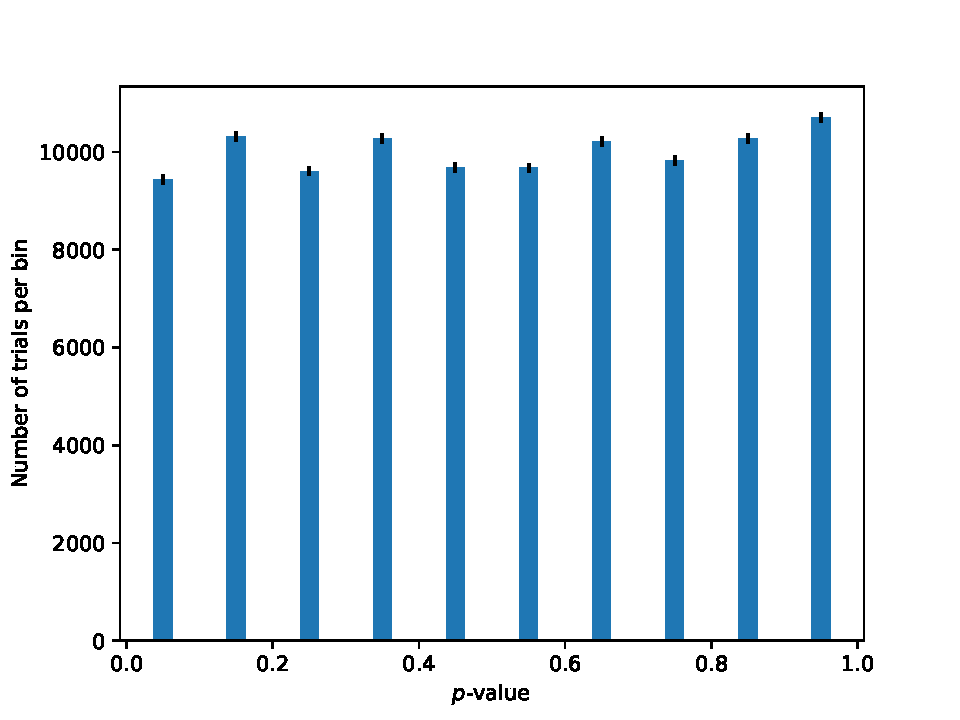
\includegraphics[width=0.8\textwidth]{figures/Hypotest/p0dist.pdf}
    \caption{Distribution of $p$-values under the hypothesis that $\epsilon=0.9$. The error bars indicate the standard deviation of the a Poisson whose mean equals the number of observed entries in each bin.}
    \label{fig:p0dist}
\end{figure}

Of course we might also be interested in finding a better estimate of the efficiency, rather than testing a single efficiency. All possible values of efficiencies $\epsilon \in [0,1]$ would then form a composite hypothesis. We'll come on to this later on, but first we need to introduce a fundamental concept in hypothesis testing - the likelihood function. 

\subsection{Likelihoods}
The likelihood function is a very powerful tool in statistics, and as a particle physicist will be your go-to when performing statistical inference. We've come across it already in Bayes' theorem when applied to experimental data (Eqn.~\ref{eqn:bayesexp}). 

The likelihood function $L$ is defined by, 
\begin{equation}\label{eqn:likelihood}
L(\theta) \propto P(X|\theta).
\end{equation}
The likelihood is defined for a fixed observation $X$ and is proportional to the probability to observe $X$, given a value of some parameter set $\theta$. The likelihood function is a \emph{function of the parameters} $\theta$. Note that we write a proportionality rather than an equality because the likelihood function is \emph{not} a probability density. In practice, we often only care about ratios of likelihoods for different values of the parameter(s) and hence we almost never care about this constant of proportionality. 

For $N$ independent observations $\mathbf{X}=\{X_{1},X_{2},...,X_{N}\}$, the likelihood function is, 
\begin{equation}\label{eqn:likelihoodprod}
L(\theta) := \prod_{i=1}^{N}f_{i}(X_{i};\theta),
\end{equation}
where $f_{i}$ are the p.d.f for each observation.

In HEP, we often make the distinction between  \emph{binned} likelihood and \emph{un-binned} likelihoods. To get the most out of the data, the un-binned likelihood is always better, however there may be restrictions that mean the binned likelihood is more appropriate. For example, if using MC simulation to estimate the distribution of some process, you may only be able to bin the simulation and hence you'll need to use a binned likelihood. Also, you might find that for computation, the binned likelihood is faster - this is usually the case if you have many events in your dataset. We'll see examples of both binned and un-binned likelihoods later, but for now, we need to cover an extremely important result, which unites likelihood functions and hypothesis testing.

\subsection{Neyman-Pearson Lemma}
Let's go back to the problem of finding the most powerful test of our null hypothesis $H_0$ against an alternate hypothesis $H_1$. As we've seen, we can state this problem as finding the \emph{best critical region} $w$. Let $\mathbf{X}$ be our observation (experimental data) and suppose it has a p.d.f $f(\mathbf{X};\theta)$, where $\theta=0$ represents the null hypothesis $H_0$ and $\theta=1$ represents the alternate hypothesis $H_1$. Note that I will reserve the notation $f(X|H)$ for only when $H$ represents a hypothesis for which $f(X|H)$ yields the distribution under which $X$ is distributed assuming $H$ is true -- very often in HEP, this is the same as setting some parameter values so that $f(X|H(\theta))=f(X;\theta)$ but i'll try not to confuse these notations. 

For a specific $\alpha$ we choose $w$ such that,
\begin{equation}\label{eqn:nptestsize}
    \int_{w}f(\mathbf{X};\theta_0)d\mathbf{X} = \alpha,
\end{equation}
and we want to find the region $w$ which maximises $1-\beta$. We can write Eqn.~\ref{eqn:power} as, 
\begin{eqnarray}\label{eqn:nppower}
    1-\beta & = &\int_{w}f(\mathbf{X};\theta_1)d\mathbf{X}\\
            & = &\int_{w}\frac{f(\mathbf{X};\theta_1)}{f(\mathbf{X};\theta_0)}f(\mathbf{X};\theta_0)d\mathbf{X}\\ 
            & = & E\left[\frac{f(\mathbf{X};\theta_1)}{f(\mathbf{X};\theta_0)}\bigg|\theta=\theta_0\right]_{w},
\end{eqnarray}
where the last line denotes the expectation value inside $w$, under the null hypothesis of the quantity,
\begin{equation}
\Lambda=\dfrac{f(\mathbf{X};\theta_1)}{f(\mathbf{X};\theta_0)}=\dfrac{L(\theta_1)}{L(\theta_0)}.
\end{equation}
This quantity is the ratio of the likelihood function, evaluated under the two hypotheses. The expectation in Eqn.~\ref{eqn:nppower} will be maximal when $w$ is chosen to contain the largest values of $\Lambda$. Thus, the best critical region is the set of points for which $\Lambda \geq c_{\alpha}\in \mathbb{R}$, where $c_{\alpha}$ satisfies Eqn.~\ref{eqn:nptestsize}. If $\Lambda>c_{\alpha}$, we would choose $H_{1}$, while $\Lambda \leq c_{\alpha}$ leads us to choose $H_0$. 

Often, given that this test is the most powerful, you will find that in HEP we use $\Lambda$ as \emph{the} test statistic, even if the hypotheses that we're testing are not simple ones. You should note however that the Neyman-Pearson lemma only applies to simple hypotheses and that $\Lambda$ is not necessarily the most optimal test statistic for other hypotheses -- in practice it turns out to have extensions which are extremely convenient so we still use ratios of likelihood functions ubiquitously in HEP. 


\subsection{Nuisance parameters}
So far we've talked about testing \emph{simple} hypotheses. As with most things in real life, the hypotheses that we want to test in particle physics are anything but simple. More often than not, we test \emph{composite} hypotheses against one another. Composite hypotheses can be thought of as a set of hypotheses that are parameterised by one (or more) parameters, often related to parameters of a physical model we are interested in. These parameters might correspond to the cross-section of some particle interaction process or the mass of a particle, or even some SUSY parameter like $\tan\beta$. In experimental particle physics, we also encounter parameters related to our experimental setup. These might be calibration coefficeints of the calorimeter, efficiencies on our event selection or the flux of a neutrino beam. Usually we are not so interested in defining the hypothesis with regards to all of these later parameters. We split the parameters of the model into two sets, $\theta=(\mu,\eta)$. The parameters $\mu$ are the \emph{parameters of interest} and typically correspond to the parameters that represent the set of hypotheses we are interested in testing. Instead, the parameters $\eta$ represent those parameters which we don't care about -- these are the \emph{nuisance parameters}. Typically, nuisance parameters are \emph{measured}, and we can think of those measured values as being random variables in their own right. The probability density function for them has two interpretations. Either you think of them as part of the likelihood itself, in which case particle physicists usually refer to them as \emph{external constraint terms}, or they simply represent our prior knowledge of the nuisance parameters -- practically this interpretation doesn't really matter but it can help when discussing with other particle physicists. Sometimes however, we have no prior knowledge about (one or more of) the nuisance parameters and in this case, they will not appear or will have flat priors.

Our composite hypotheses will be labelled as $H(\mu)=H\left(\mu,\eta(\mu)\right)$ meaning in order to specify the hypotheses corresponding to different values of $\mu$, we must make a choice of what to do with $\eta$, which can depend on the value of $\mu$. For dealing with experimental data, we will be using the likelihood function
and the choice boils down to one of two procedures, \emph{profiling} and \emph{marginalisation}. Typically, you will encounter profiling in frequentist procedures, and marginalisation in Bayesian procedures. There are however some procedures which have been used in the past that mix the two methods together (and it can make sense to do so), so we will just stick to calling them profiling or marginalising.

\paragraph{Profiled likelihoods}
Profiling the likelihood can sometimes be thought of selecting the ``best'' value of the nuisance parameters for any value of the parameters of interest. The definition of ``best'' here means that which maximises the likelihood for a particular value(s) of $\mu$. We'll see later that this choice will have useful implications, but for now, know that this is \emph{the choice} for frequentists. We start by taking twice the negative of the log-likelihood function,
\begin{equation}
    q(\mu,\eta)= -2\ln L(\mu,\eta).
\end{equation}
We then choose $\eta(\mu)$ as $\hat{\eta}_{\mu}$, which represents the values of $\eta$ for which $q$  minimized when evaluated at $\mu$. Specifically,
\begin{equation}
\hat{\eta}_{\mu} = \mathrm{arg min}_{\eta}\left\{q(\mu,\eta)\biggr|_{\mu}\right\},
\end{equation}
meaning we first fix $\mu$ and then find the values of $\eta$ which minimize $q$. If it's not clear, don't worry, we'll make it clear with an example soon. We then write the \emph{profiled log-likelihood} as,
\begin{equation}
q(\mu) = q(\mu,\hat{\eta}_{\mu}),
\end{equation}
to remove the $\eta$ dependence from the likelihood. Note that we've not specified the likelihood here, and we could have separated it into two components; $L(\mathrm{data}|\mu,\eta)\cdot L(\eta_{\mathrm{measured}}|\eta)$. The term $L(\eta_{\mathrm{measured}}|\eta)$ is the constraint term, which typically arises from some previous measurement of $\eta$, $\eta_{\mathrm{measured}}$. Often in HEP, we parameterize the likelihood so that $\eta_{\mathrm{measured}}=0$ and $L(\eta_{\mathrm{measured}}|\eta)\propto \prod_{i=1}^{M}\phi(0,1)$ for $M$ independent measurements (relying on the CLT to justify the choice of normal distributions), but this is just technicalities and we shouldn't get bogged down in this.

\paragraph{Marginalised posteriors}\label{sec:marginalised}
Marginalisation is the second way to deal with nuisance parameters. As before, we begin with the likelihood function $L(\mu,\eta)$. This time however, we separate out our prior knowledge of the nuisance parameters from the experimental data, plug into Bayes' theorem to obtain the posterior function and \emph{integrate} over the nuisance parameters,
\begin{equation}\label{eqn:bayesmargin}
P(\mu) = \frac{\int L(\mathrm{data}|\mu,\eta)\pi(\mu)\pi(\eta) d\eta}{P(\mathrm{data})},
\end{equation}
where $P(\mathrm{data})$ is the usual normalisation term $P(\mathrm{data})=\int\int L(\mathrm{data}|\mu,\eta)\pi(\mu)\pi(\eta) d\eta d\mu  $, and $\pi(\mu)$ and $\pi(\eta)$ are the \emph{prior probability densities} for $\mu$ and $\eta$.  Rather than choosing a single value of $\eta$ for each $\mu$, we've integrated over them, weighted according to the prior distribution. Thus the marginalised posterior is the expectation value of the posterior at each value of $\mu$. Here is where we need to be careful about the choice of priors, as our results can change depending on this choice. Any inference based on marginalised posteriors needs to include a study of the dependance on these priors. Typically in HEP, we tend to use \emph{flat} priors for $\mu$ and (similarly to the profiling case), normal priors for $\eta$. The latter is justified if there are external measurements of $\eta$, but ``flat'' for a parameter $\mu$ is not flat for a parameter $\mu^{2}$ -- it's not always obvious which is the more fundamental thing which we should have no prior knowledge about. For example, a cross-section is often proportional to a $\mathrm{(coupling)}^{2}$ but which one should be flat? The main thing is to make sure the final results are not very sensitive to this, otherwise explaining the choice of priors is vital for any paper.

In both cases we can now make statements about $H(\mu)$ either through the profiled likelihood $q(\mu)$ or the posterior $P(\mu)$ as the nuisance parameters $\eta$ have been eliminated. In the next section, we'll take a look at a concrete example to (hopefully) make it a more clear as to what we would do (practically) in both cases.

\subsection{A counting experiment}
To demonstrate profiling and marginalisation, we will use a very simple counting experiment. Counting experiments in HEP, simply mean that the observation (data) is just a single number $n$ -- the observed event count, and all of the model parameters are included inside the Poisson parameter $\lambda$. For a typical particle physics experiment, we want to study the rate of some particle X, produced in proton-proton collisions $pp\rightarrow\mathrm{X}$. We often have a theoretical prediction for the cross-section $\sigma(pp\rightarrow \mathrm{X})$, acceptance $A$ for our detector, efficiencies $\epsilon$ for our selection and a total integrated luminosity $l$. We usually introduce a scaling parameter $\mu$ that will parameterise different hypotheses. $\mu=1$ corresponds to the rate of the process being exactly as our theory colleagues predicted, while a value of $\mu=0$ means the process never occurs. There is almost always some background contribution $B$ so that the total rate can be written as,
\begin{equation}\label{eqn:lambdanom}
    \lambda(\mu) = \mu\sigma(pp\rightarrow \mathrm{X}) A\epsilon l + B,
\end{equation}
Nuisance parameters arise in counting experiments due to any one of the terms in Eqn.~\ref{eqn:lambdanom} being imprecisely known (or not at all). They are usually always parameterised using a \emph{log-normal} distribution. This is very common in HEP. If a random variable $\eta$ is distributed (or constrained by) a normal distribution with a mean of 0 and variance of 1, then $l=l_{0}(1+k)^{\eta}$ will be distributed as a log-normal and $\ln(l)$ will be normally distributed with a mean of $l_{0}$ and a variance of $k^{2}$. The nice thing about log-normals is that $l(\eta)$ parameterised in this way can \emph{never} be negative and hence neither can the Poisson mean. It's quite intuitive to think of this uncertainty having a relative effect - for example a 100\% uncertainty on $l$ means we know $l$ within a factor of 2 (we don't say that we think $l$ could be zero!). Furthermore, the smaller the value of $k$, the more $l(k)$ can be approximated by a normal distribution. Say then that our luminosity has some relative uncertainty $k$, we then write our Poisson mean as,
\begin{equation}
    \lambda(\mu,\eta) = \mu\sigma(pp\rightarrow \mathrm{X}) A\epsilon l(1+k)^{\eta} + B,
\end{equation}
Now we can use our two approaches to deal with this nuisance parameter. First, we'll take the profiling approach. The likelihood that we'll profile is,
\begin{equation}\label{eqn:lhcounting}
    L(\mu,\eta) = \lambda(\mu,\eta)^{n}e^{-\lambda}\cdot e^{-\frac{1}{2}\eta^{2}},
\end{equation}
where we've dropped any terms that are constant in $\mu$ and $\eta$. The term  $e^{-\frac{1}{2}\eta^{2}}$ is our constraint term for $\eta$. We now take twice the negative log,
\begin{equation}
    q(\mu,\eta) = -2\ln L(\mu,\eta) = \eta^{2}+2\lambda(\mu,\eta)-2n\ln\lambda(\mu,\eta).
\end{equation}
Minimizing $q(\mu,\eta)$ is the same as maximising $L(\mu,\eta)$. We could use any number of minimisation programs to do this for us, but since this problem is quite simple, we can code up a simple Newton method to find the solution to $q'=\frac{\partial q}{\partial \eta}=0$. In the Newton algorithm, from an initial starting point, $\eta_0$, the next point is proposed as $\eta_1=\eta_0-\frac{q'(\eta_{0}}{q''(\eta_0)}$. We iterate until $|q'|<\delta$ picking some tolerance. We can analytically calculate,
\begin{eqnarray}
    q'  =  \frac{\partial q}{\partial \eta} & = &   
    2\eta 
    +2\frac{\partial\lambda}{\partial \eta} 
    - \frac{2n}{\lambda}\frac{\partial\lambda}{\partial \eta} = 
    2\eta 
    + 2\ln(1+k) \left(\lambda-B\right)
    -2n\ln(1+k)\frac{\lambda - B}{\lambda}\\
    q''  =  \frac{\partial ^{2}q}{\partial \eta^{2}} 
    & = &   
    2 
    + 2\ln(1+k)\frac{\partial\lambda}{\partial \eta} 
    - 2n\ln(1+k)\left( \frac{B}{\lambda^{2}}\frac{\partial\lambda}{\partial \eta}  \right)
    = 
    2 
    + 2(\ln(1+k))^{2}\left(\lambda-B\right)\left( 1-\frac{nB}{\lambda^{2}}\right),
\end{eqnarray}

where we've used the fact that $\frac{\partial\lambda}{\partial \eta} =\ln(1+k)(\lambda-B)$.

For each value of $\mu$, we can find $\hat{\eta}_{\mu}$ as the solution to $\frac{\partial q}{\partial \eta}\biggr|_{\mu}=0$.

For marginalisation, we again start with the likelihood, but this time, we maintain all of the terms
\begin{eqnarray}
    L(n|\mu,\eta) & = & \frac{\lambda(\mu,\eta)^{n}}{n!}e^{-\lambda}\\
    P(\eta) & = & \frac{1}{\sqrt{2\pi}}e^{-\frac{1}{2}\eta^{2}}\\
    \pi(\mu) & = & \begin{cases}
                \frac{1}{15} & \mu \in (-1,15) \\
                0 & \mathrm{else,}
                \end{cases}
\end{eqnarray}
and we simply plug these into Eqn.~\ref{eqn:bayesmargin} to obtain the posterior $P(\mu)$. Here we've chosen a wide prior for $\mu$ so as to not affect the posterior.

Now suppose you've called your colleagues up in Durham and they've sent over a theoretical prediction for the cross-section $\sigma(pp\rightarrow \mathrm{X}) = 0.01$pb. You also know your apparatus well and know that for this process, the efficiency of your selection will be $\epsilon=0.9$ and the acceptance $A=0.5$. You collide protons until you reach a total integrated luminosity of $l=100\mathrm{pb}^{-1}$. You don't know the luminosity perfectly, but it has been measured to within 10\%, so $k=0.1$. The backround rate is known to be $B=0.5 $. After running the experiment, we observe 2 events. Below is some code which defines this setup. We can save this in a file called \textsf{model.py} so that we can import it later rather than redefine each time.
\begin{lstlisting}[style = Python]
sigma_TH = 0.01
A = 0.5 
eff = 0.9 
l = 100. 
k = 0.1 
B = 1.0
n   = 2

# Poisson mean
def lamb(mu,eta):
  return mu*eff*A*l*((1+k)**eta)*sigma_TH + B
\end{lstlisting}

To calculate the profile likelihood in our simple counting experiment, we use the Newton method. Figure~\ref{fig:profiledlikelihoodex_counting} can be produced 
by following the notebook \href{https://github.com/nucleosynthesis/PGStatistics/blob/main/notebooks/ProfilingVsMarginalisation.ipynb}{\textsf{ProfilingVsMarginalisation.ipynb}}.

\begin{figure}[hbt!]
    \centering
    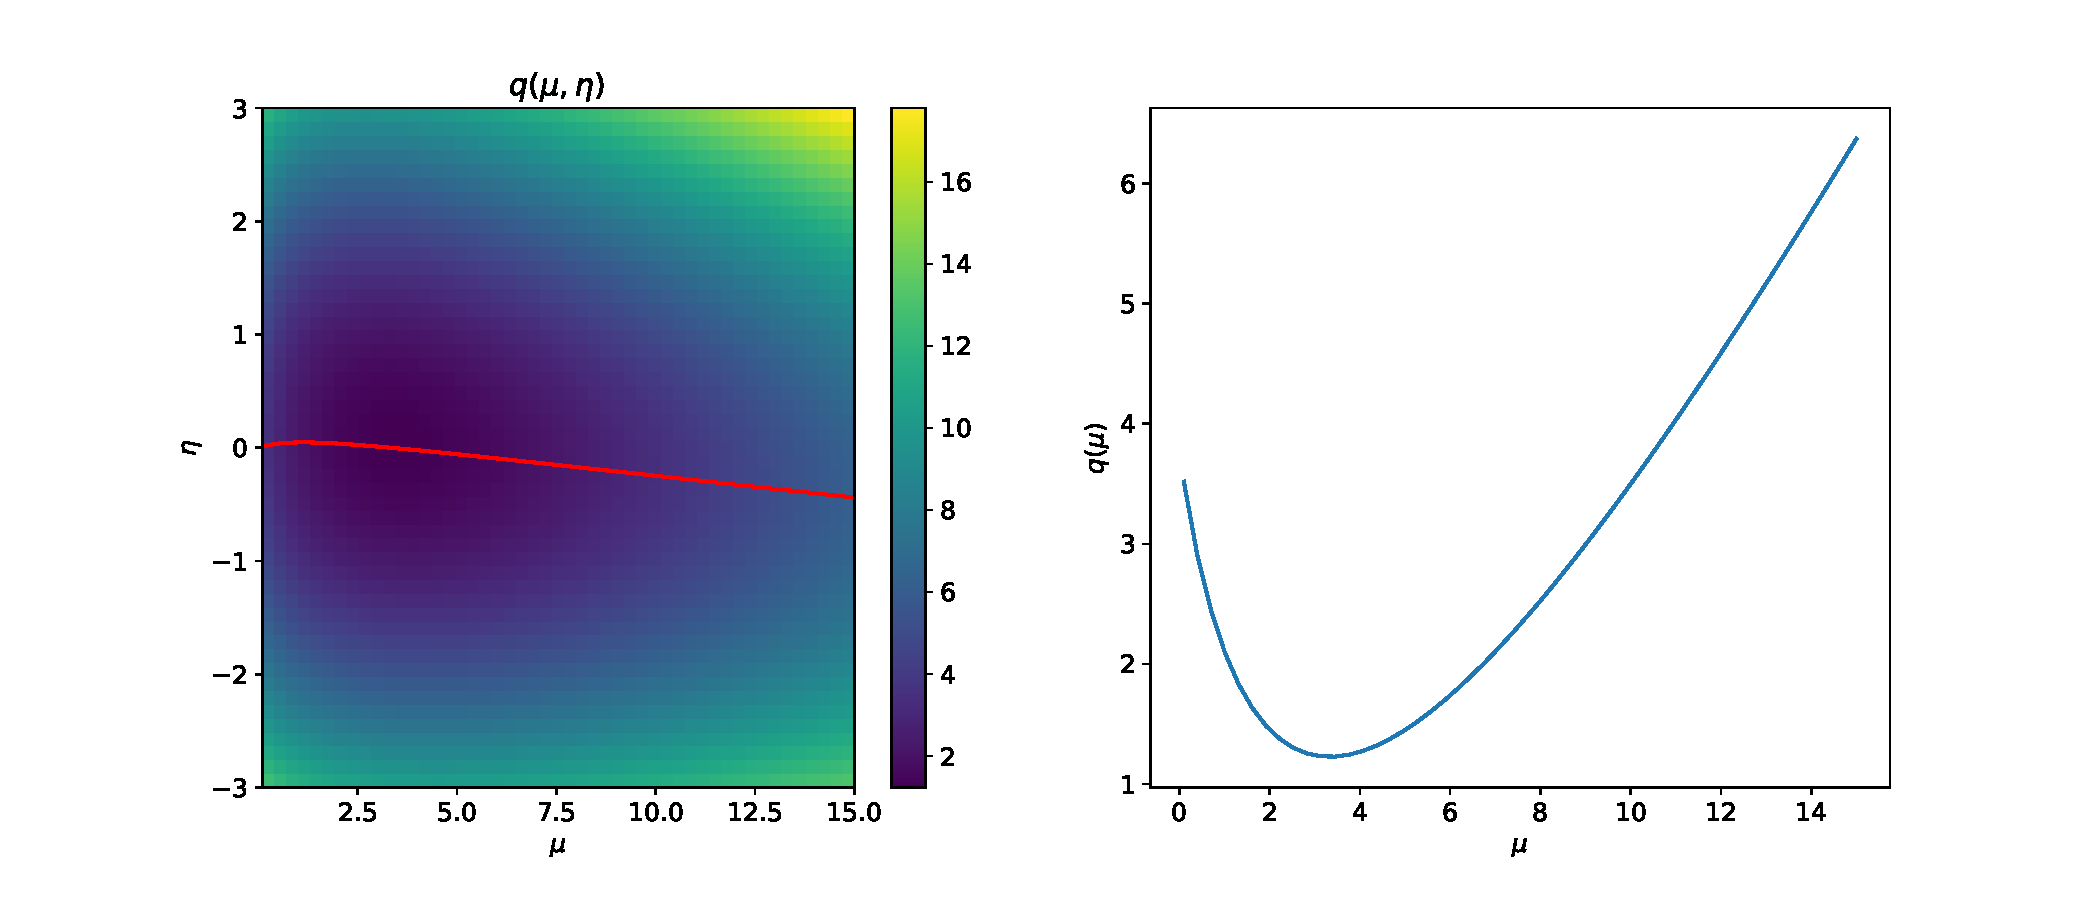
\includegraphics[width=\textwidth]{figures/Hypotest/prof_lh_ex.pdf}
    \caption{Left: Twice negative log-likelihood function for the counting experiment vs 
    $\mu$ and $\eta$. The red line shows the profiled value of the nuisance parameter at each value of $\mu$ $\hat{\eta}_{\mu}$. Right: the profiled log-likelihood function $q(\mu)$.}
    \label{fig:profiledlikelihoodex_counting}
\end{figure}

If instead, we want to obtain the marginalised posterior function, 
we can use the \textsf{scipy.integrate.quad} methods 
to perform the integration numerically. An example code for 
producing the marginalised posterior is below, and the output 
from the code is shown in Figure~\ref{fig:marginalised_ex_counting}. 
Again, you can follow the 
\href{https://github.com/nucleosynthesis/PGStatistics/blob/main/notebooks/ProfilingVsMarginalisation.ipynb}{\textsf{ProfilingVsMarginalisation.ipynb}} 
notebook to see how this works. In that notebook, the posterior distribution is also computed 
using the Markov chain MC method that we covered in section~\ref{sec:MarkovChain}. 


\begin{figure}[hbt!]
    \centering
    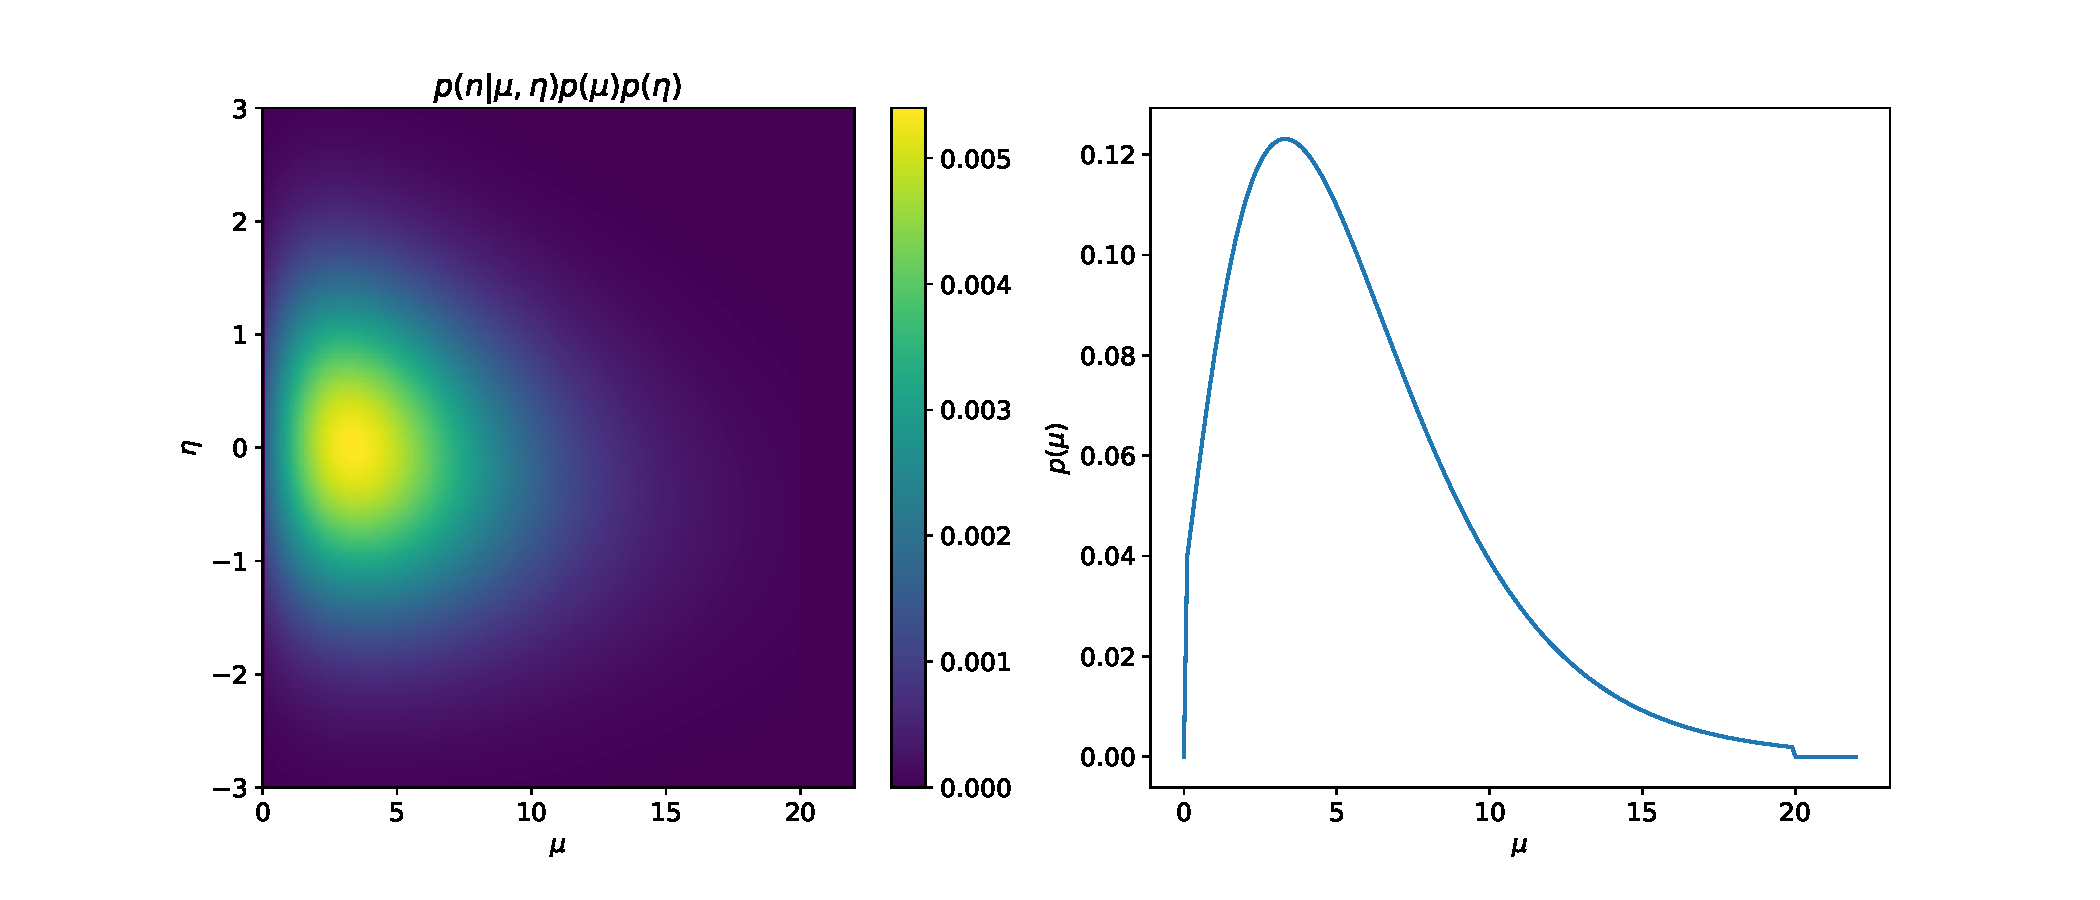
\includegraphics[width=\textwidth]{figures/Hypotest/marginalised_lh_ex.pdf}
    \caption{Left: Likelihood function multipltied by priors on $\mu$ and $\eta$ for the counting experiment vs $\mu$ and $\eta$.  Right: the marginalised posterior function $P(\mu)$.}
    \label{fig:marginalised_ex_counting}
\end{figure}

For Bayesians, having the posterior, now only as a function of the parameter of interest, is enough to perform statistical inference, such as hypothesis tests. One question that you'll probably have to ask (unfortunately) is which hypotheses can we exclude (reject) with some error rate $\alpha$ given the data observed? In the case where we have parameterised the set of hypotheses with parameter $\mu$, we can ask which values of $\mu$ can be rejected. For an example such as the counting experiment, we can also ask what the \emph{largest} value of $\mu$ (and hence which set of $H(\mu)$) can be rejected with error rate $\alpha$. This is referred to as an \emph{upper limit} on $\mu$, and the Bayesian would calculated it as $\mu_{\mathrm{up}}$ satisfying, 
\begin{equation}
    \int_{-\infty}^{\mu_{\mathrm{up}}}P(\mu)d\mu = 1-\alpha,
\end{equation}
where in practice, one rarely needs to use $-\infty$ as a lower bound. With this, we can reject all hypotheses $\left\{H(\mu):\mu>\mu_{\mathrm{up}}\right\}$ at an error rate of $\alpha$ or less. 

Bayesians would say that this is the upper limit on $\mu$ with $100\times(1-\alpha)$\% credibility. The equivalent from frequentists would be to determine the upper limit on $\mu$ with $100\times(1-\alpha)$\% confidence level. We'll come back to credible intervals and confidence intervals later on. But for now, we need to do a bit more work for the frequentists, and at the same time we'll introduce the standard tools for setting upper limits in HEP. 

\subsection{Upper limits and common HEP test statistic}
As we've mentioned already, profiled likelihoods (and ratios of them) are very common in hypothesis testing, due to the Neyman-Pearson lemma. In HEP, and in particular at the LHC, there is a standard test statistic used to set upper limits on cross-sections/signal-rates. The first step, is to identify a signal scaling parameter as we had done in the previous section -- $\mu$. Typically when searching for a new phenomena. 

We mentioned the idea of excluding a particular hypothesis $H(\mu)$ at a given confidence level $1-\alpha$ by finding an upper limit on $\mu$. We can think of this as a series of tests, one for each value of $\mu$
and deciding whether to reject it or not, with a given error rate $\alpha$. In each of these tests, our \emph{null} hypothesis is $H(\mu)$ since we are asking whether or not we can reject it. Clearly $H(0)$ is the \emph{background only} hypothesis, and usually we parameterise the signal such that $H(1)$ corresponds to some theoretical prediction. If we exclude all $\mu\geq 1$ (i.e $\mu_{\mathrm{up}}<1)$ , we have excluded this theoretical model. 

We also need an alternate hypothesis, and for that, we use the $\emph{best}$ value of $\mu$ given the observed data - $\hat{\mu}$. Again, this means finding the value of $\mu$ which (minimises) maximises the (log)likelihood function. The test statistic that we use is,
\begin{equation}
    t_{\mu} = \begin{cases}
                q(\mu,\hat{\eta}_{\mu})-q(\hat{0},\hat{\eta}_{0})    & \hat{\mu} < 0 \\
                q(\mu,\hat{\eta}_{\mu})-q(\hat{\mu},\hat{\eta})    & \hat{\mu} \in (0,\mu] \\
                0               & \hat{\mu}>\mu,
                \end{cases}
\end{equation}
where we've introduced $\hat{\eta}$ to mean the \emph{global} best nuisance parameter values for any value of $\mu$. The value $q(\hat{\mu},\hat{\eta})$ is the \emph{global} minimum of $q(\mu,\eta)$. Note that there are 3 cases. The second case, is exactly our profiled likelihood, offset by the global value. The first case, imposes a constraint that $\mu<0$ is \emph{unphysical} and the third case enforces an \emph{upper limit} on $\mu$. 

For each value of $\mu$, we calculate the $p$-value, 
\begin{equation}
    p_{\mu} = \int_{t^{\mathrm{obs}}_{\mu}}^{+\infty} f(t_{\mu}|H(\mu))dt_{\mu},
\end{equation}
where $f(t_{\mu}|H(\mu))$ is the distribution of $t_{\mu}$ under the hypothesis $H(\mu)$ is true typically calculated using MC methods, and $t^{\mathrm{obs}}_{\mu}$ are the values of $t_{\mu}$ for the observed data. This particular test statistic has the added bonus that the distribution can be determined analytically in the asymptotic (normal approximation) limit, meaning we don't need to use MC to determine $f(t_{\mu}|H(\mu))$\footnote{You can find these formula in the paper ``Asymptotic formulae for likelihood-based tests of new physics'', \href{https://arxiv.org/abs/1007.1727}{DOI: 10.1140/epjc/s10052-011-1554-0}}, saving us a lot of computing time.

Let's apply this to our simple example counting experiment using a MC method. The first thing is to decide how we are going to generate pseudo-experiments (toys) to determine $f(t_{\mu}|H(\mu))$. We have again encountered the problem that $H(\mu)$ is defined only for a fixed choice of the nuisance parameters $\eta$. Once again, we'll turn to our choice of the \emph{best} values, meaning we will pick those which minimises $q(\mu,\eta)$ for a given value of $\mu$ given our observed data. We already calculated these, it's the red line in Figure~\ref{fig:profiledlikelihoodex_counting} -$\hat{\eta}_{\mu}$. For each toy, we want to generate a random value of the observation $n'$, given $\mu,\hat{\eta}_{\mu}$ and a value of $\eta'$ which represents the random outcome for $\eta$ our luminosity measurement - remember, in the frequentist view, the value that we obtained can also be interpreted as a random variable with a known distribution $\eta{^{\prime}}\sim\phi(\hat{\eta}_{\mu},1)$ -- our observed data then becomes $(n^{\prime},\eta^{\prime})$. We need to modify the likelihood function of Eqn.~\ref{eqn:lhcounting} for each toy slightly to read, 
\begin{equation}
    L(\alpha,\eta) = L(n^{\prime},\eta^{\prime}) = \lambda(\mu,\eta)^{n\prime}e^{-\lambda}\cdot e^{-\frac{1}{2}(\eta-\eta^{\prime})^{2}},
\end{equation}
For each toy, we can then calculate $t_{\mu}$ using this data in the likelihood function and histogram the results. Note that for each toy, we will find different values of $\hat{\mu}$ and $\hat{\eta}_{\mu}$! 

Follow the \href{https://github.com/nucleosynthesis/PGStatistics/blob/main/notebooks/FrequentistUpperLimits.ipynb}{FrequentistUpperLimits.ipynb} notebook for an example where we calculate the 95\% confidence level upper limit for $\mu$ for our simple counting experiment. 

Figure~\ref{fig:tmu_example} shows example distributions of $t_{\mu}$ for the hypothesis $H(\mu=8)$ and $H(\mu=15)$. The red lines indicate the observed value $t_{\mu}^{\mathrm{obs}}$, which is used to calculate $p_{8}$ and $p_{15}$. Now, we need to calculate this distribution, and hence $p_{\mu}$ for a range of values of $\mu$. Once this is done, we can read of the value of $\mu_\mathrm{up}$ at a $100\times(1-\alpha)$ confidence level as the value of $\mu$ for which $p_{\mu}$ crosses $(1-\alpha)$. 

The result is shown in Figure~\ref{fig:pmu_example}. From here, we can find the 95\% CL upper limit by reading off where the black line crosses 0.05. 

\begin{figure}
    \centering
    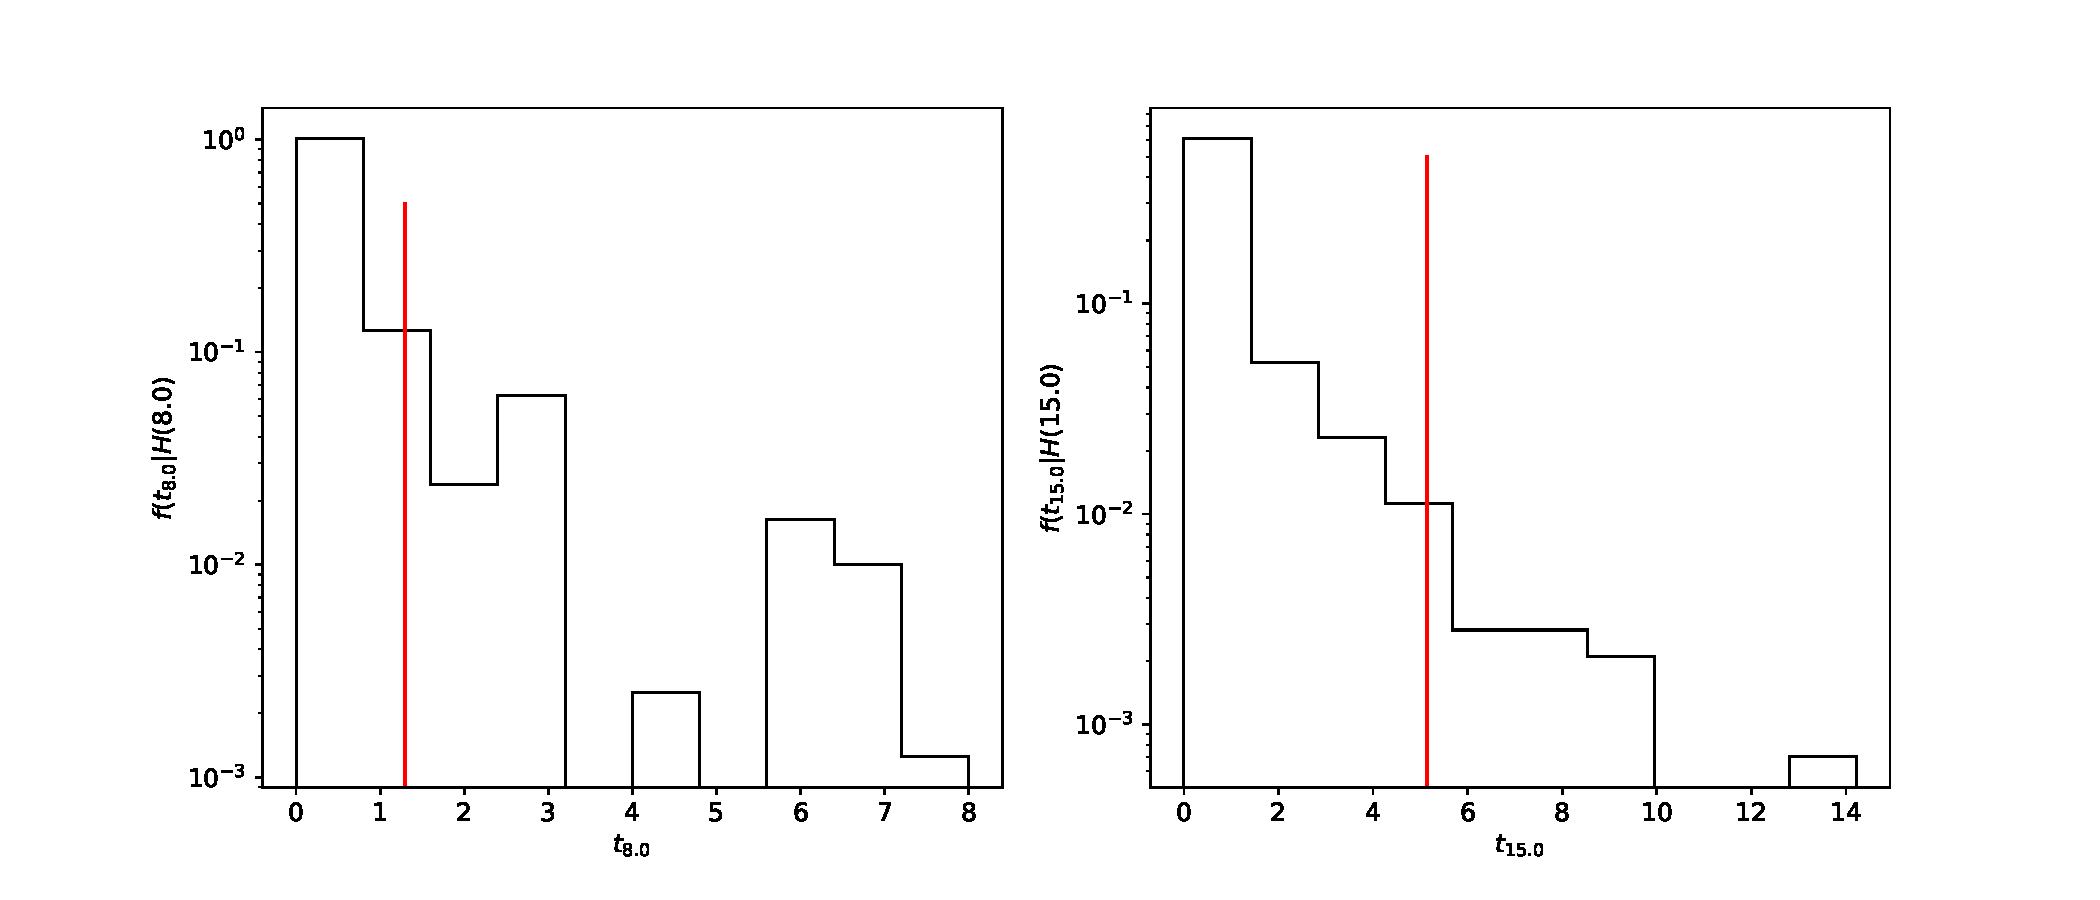
\includegraphics[width=\textwidth]{figures/Hypotest/p10.pdf}
    \caption{Example distribution of $t_{\mu}$ for $\mu=8$ (left) and $\mu=15$ (right) . The vertical red line indicates the value of  $t_{8}^{obs}$ and $t_{15}^{obs}$.}
    \label{fig:tmu_example}
\end{figure}

\begin{figure}
    \centering
    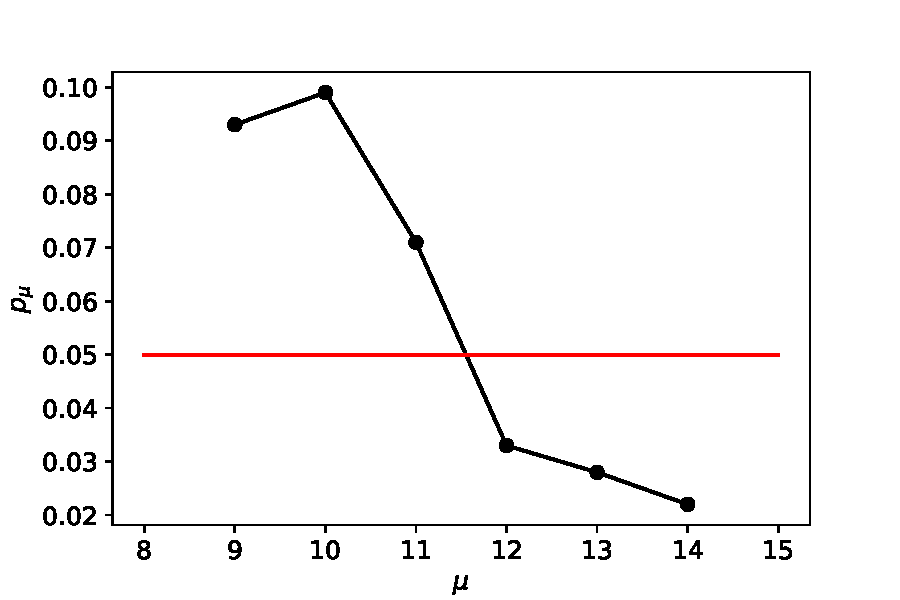
\includegraphics[width=\textwidth]{figures/Hypotest/scan_pmu.pdf}
    \caption{
    $p_{\mu}$ vs $\mu$. The horizontal red line lets us read off the value of $\mu_{\mathrm{up}}$ at the 95\% confidence level, given our observation.}
    \label{fig:pmu_example}
\end{figure}

In most real-life scenarios, you will deal with many nuisance parameters rather than just a few. In this case, I have used the \textsf{minimize} function from \textsf{scipy.optimize} (there are others like \textsf{MINUIT}, etc) which uses   gradient descent or even stochastic based routines to find the (log)likelihood extrema. For marginalisation, integration is typically performed using MC methods such as the Markov chain approach. As I mentioned at the start, these lectures aren't about these tools, but feel free to ask me/your colleagues about them when you start your Ph.D research. 

You will most likely come across the $CL_{S}$ criterion during your Ph.D. Using  the $CL_{S}$ criterion  means that instead of basing the test on $p_{\mu}$, we base it on the value of $CL_{S}=\frac{p_{\mu}}{1-p_{b}}$ compared to $\alpha$, where 
\begin{equation}
    p_{b} = \int_0^{t^{\mathrm{obs}}_{\mu}}  f(t_{\mu}|H(0))dt_{\mu}.
\end{equation}
We won't dwell on this too much but you should know that $CL_{S}$ is known to \emph{over-cover} (what does that even mean? Don't worry, we'll get to it) and is designed to avoid excluding a signal hypothesis when the data disagrees with the background-only hypothesis and the signal plus background hypothesis, when the two look very similar. Now that I've started to introduce words like \emph{cover}, we should move on to explaining credible/confidence intervals and the concept of $\emph{coverage}$. 
\section{Point estimates and confidence/credible intervals}

In the previous section, we introduced the likelihood function for use in hypothesis testing and in particular rejecting hypotheses which fail some criteria based it. In this section, we'll deal with another common mode of operation for a particle physicist -- \emph{performing measurements}. In HEP, we usually report measurements of a single parameter as $X\pm\sigma_{X}$. There are a number of ways one can obtain $X$ and $\sigma_{X}$ here -- for example, it could refer to the sample mean $\bar{X}$ and standard deviation $S = \sqrt{\sum_{i}(X_{i}-\bar{X})^{2}}$ or it could refer to the moments of the distribution $f(X)$, $\mu_{1},~\sqrt{\nu_{2}}$. A very large part of what we do in HEP, is to \emph{improve on the sensitivity} of some measurement, which often involves designing experiments to measure physical quantities more precisely. Two competing experiments may claim to have measured  $X_1\pm\sigma_{X,1}$ and $X_2\pm\sigma_{X,2}$ but without knowing what they mean, we can't compare those numbers fairly. A good comparison can be made for measurements for which two properties are well understood, namely the \emph{bias} of the measured value and the \emph{coverage} of the interval. 

\subsection{Maximum likelihood estimators}
We've encountered (minimum) maximum (negative log-)likelihoods when profiling nuisance parameters. The use of maximisation/minimisation is also common in HEP when \emph{estimating} one or more parameters of interest. When choosing an estimator, a statistician will usually have in mind one or more property to be compare estimators. These can be the loss of information using a particular estimate, the variance of the estimator or even the simplicity of explaining it in a publication. What makes the \emph{maximum likelihood estimator} a good estimator is the fact that it is \emph{consistent} in the limit of large numbers, which in HEP is often the most important property. This means as the number of observations increases, the maximum likelihood estimate of a parameter converges to the real value of the parameter. Often, you'll hear particle physicists talk about the \emph{bias} of an estimator. In HEP, we often mean that either the mean ($E(\hat\theta)$) or the median of the sample distribution of $\hat{\theta}$ is equal to the true value. However, this is not quite the same thing and estimators can be unbiased but still inconsistent. For most purposes, we can however interchange the two definitions (and particle physicists will often do so as a result). We'll now show that the maximum likelihood estimate for one parameter $\theta\in\Omega$ is a consistent estimator. Note that this extends to an number of parameters, provided the likelihood function meets certain conditions (which we won't go into as in HEP it is almost always the case). 

First, recall that for multiple observations $\mathbf{X}=X_1,X_2,X_3,...,X_{N}$ of some observation, the likelihood function is defined by Eqn.~\ref{eqn:likelihoodprod}. We define the quantity $l_{N}(\theta)$, by 
\begin{equation}\label{eqn:defln}
    l_{N}(\theta) = -\frac{1}{N}\ln L(\theta) =  -\frac{1}{N}\sum_{i=1}^{N}\ln f(X_{i};\theta).
\end{equation}
Notice that minimising $l_{N}(\theta)$ is the same as maximising $L(\theta)$ since the constants have no effect on where the extreme value lies. 

By the law of large numbers, for all $\theta$, $l_{N}(\theta)\rightarrow l(\theta)$ as $N\rightarrow\infty$, where, 
\begin{equation}
    l(\theta) = E\left[-\ln(f(X;\theta))\right]_{\theta=\theta_{0}} = \int -\ln(f(X;\theta))f(X;\theta_{0})dX,
\end{equation}
and $\theta_{0}$ is the true value of $\theta$. 
The value $\theta_{0}$ is the value of $\theta$ that minimises $l(\theta)$ as can be seen from, 
\begin{eqnarray}
    l(\theta)-l(\theta_{0}) &=& \int -\ln(f(X;\theta))f(X;\theta_{0})dX- \int -\ln(f(X;\theta_{0}))f(X;\theta_{0})dX \\
     & = & \int -\ln\left(\frac{f(X;\theta)}{f(X;\theta_0)}\right)f(X;\theta_{0})dX\\
     & = & E\left[-\ln\left(\frac{f(X;\theta)}{f(X;\theta_0)}\right)\right]_{\theta=\theta_{0}} 
      \geq  -\ln\left( E \left[\frac{f(X;\theta)}{f(X;\theta_0)}\right]_{\theta=\theta_{0}}\right),
\end{eqnarray}
where in the last step, we've used Jensen’s inequality for the expectation of strictly convex functions, knowing that $-\ln(\cdot)$ is a convex function. Now we notice that, 
\begin{equation}
    \ln\left( E \left[\frac{f(X;\theta)}{f(X;\theta_0)}\right]_{\theta=\theta_{0}}\right) = \ln\left(\int \frac{f(X;\theta)}{f(X;\theta_0)}f(X;\theta_{0})dX\right) = \ln\left(\int f(X;\theta)dX\right) = \ln(1) = 0,
\end{equation}
so that, 
\begin{equation}
l(\theta)-l(\theta_{0}) \geq 0
\end{equation}
for all $\theta$ -- meaning $\theta_0$ is the value of $\theta$ that minimises $l(\theta)$. We have that for each $N$ $\hat{\theta}_{N}$ is the value of $\theta$ that minimises $l_{N}(\theta)$ and we know that $l_{N}(\theta)\rightarrow l(\theta)$ as $N\rightarrow \infty$. If the maximum likelihood estimates $\hat{\theta}$ are unique, it can be shown that $\hat{\theta}_{N}\rightarrow\theta_{0}$  as $N\rightarrow \infty$, which would prove that the maximum likelihood estimate (or minimum log-likelihood estimate) is consistent. While we won't explicitly prove this last part, it is intuitive since the sequence of likelihood functions $l_{N}$ will have minimum values that get arbitrarily close to the minimum value of $l$. Since only one value of $\theta$ minimises these functions, it makes sense that these values also get arbitrarily close to $\theta_0$.  

As we've seen (only in 1-dimension so far), obtaining the minimum log-likelihood estimates for parameters $\vec{\theta}$ can be done numerically by solving the set of equations \begin{equation}
    \nabla_{\vec{\theta}}~q(\vec{\theta}) = 0,
\end{equation} 
and we refer to the solutions as $\hat{\vec{\theta}}$. We'll take a look at a simple example to demonstrate the maximum likelihood estimator as a consistent estimator. 

\begin{tcolorbox}[colback=backblue]
\textbf{Example:} Suppose we want to estimate the two parameters $\vec{\theta} = (\mu, \sigma)$ of a normal distribution, $\phi(X;\mu,\sigma)$ given a set of observations $X_1,X_2,...,X_{N}$. The likelihood function is, 
\begin{equation}
    q(\mu,\theta) = -2\sum_{i=1}^{N}\ln\left( \frac{1}{\sigma\sqrt{2\pi}}e^{-\frac{1}{2}\left(\frac{X_{i}-\mu}{\sigma}\right)^{2}}\right) = N\ln(\sigma\sqrt{2\pi})+\sum_{i=1}^{N}\left(\frac{X_{i}-\mu}{\sigma}\right)^{2}.
\end{equation}
Suppose the true values are $\mu_{0}$ and $\sigma_{0}$. The code below shows how we can generate $N$ values of $X$ and find the maximum likelihood estimates  $\hat{\mu}$ and $\hat{\sigma}$ for increasing $N$. We'll use the \textsf{minimize} function from the \textsf{scipy.optimize} package.
\begin{lstlisting}[style = Python]
import numpy
from scipy.optimize import minimize
import matplotlib.pyplot as plt
plt.rcParams.update({'font.size': 14})

# true values
mu_0     = 4.0
sigma_0  = 2.0

# empty list of data for now
data = []

def q(params_list = []):
   mu    = params_list[0]
   sigma = params_list[1]
   N = len(data)
   sum_part = sum( [ ((x-mu)/sigma)**2 for x in data ] )
   return 2*N*numpy.log(sigma*((2*numpy.pi)**0.5)) + sum_part

# inital values for mu, sigma
init_params = [mu_0,sigma_0]
bounds  = [(-10,10),(0.01,10)]
# generate random data
steps = [5,10,20, 50, 100, 200, 500, 1000, 5000, 10000, 20000]
hat_mu = []; hat_sigma = []
for N in steps:
  data = numpy.random.normal(mu_0,sigma_0,size=N)
  mle = minimize(q,init_params,bounds=bounds)
  hat_mu.append(mle.x[0])
  hat_sigma.append(mle.x[1])

plt.plot(steps,hat_mu,color='blue',marker="o",label="$\hat{\mu}$")
plt.plot(steps,hat_sigma,color='red',marker="o",label="$\hat{\sigma}$")

plt.plot(steps,[mu_0 for s in steps],color='blue',linestyle="--")
plt.plot(steps,[sigma_0 for s in steps],color='red',linestyle="--")

plt.xlabel("N")
plt.ylabel("$\hat{\mu}$ or $\hat{\sigma}$")

plt.xscale('log')
plt.legend()
plt.show()
\end{lstlisting}
The results are shown in Figure~\ref{fig:example_mle_normal}. Clearly as $N$ increases, the maximum likelihood estimates for $\mu$ and $\sigma$ get closer to the true values.
\end{tcolorbox}
\begin{figure}[hbt!]
    \centering
    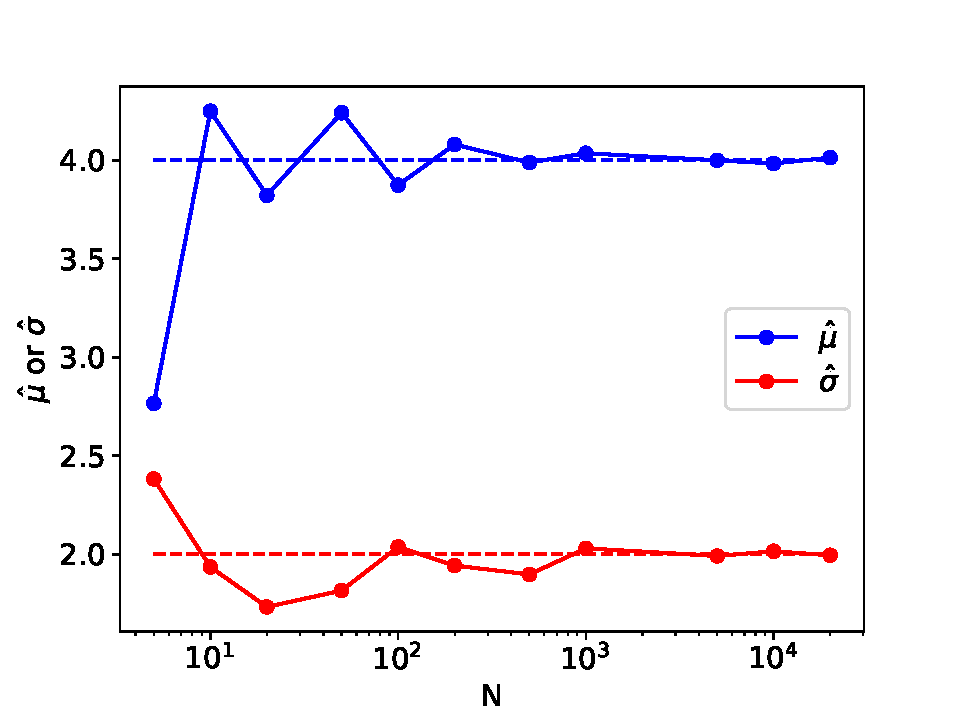
\includegraphics[width=0.8\textwidth]{figures/Intervals/Consistency_normal.pdf}
    \caption{Maximum likelihood estimates for the two parameters of a normal distribution. The likelihood is calculated from $N$ observations and the maximum likelihood estimates are determined for increasing values of $N$.}
    \label{fig:example_mle_normal}
\end{figure}
Note that in the example, we didn't need to specify whether the parameters were parameters of interest or nuisance parameters. Now we know what the $X$ refers to when a particle physicist reports a measurement as $X\pm\sigma_{X}$ -- more often than not, he/she has reported the \emph{maximum likelihood estimate} of the parameter $X$.  We are ready to discuss what the $\sigma_{X}$ means. 

\subsection{Neyman construction and frequentist confidence intervals}
The frequentist approach to reporting uncertainties on measurements is to consider the uncertainty itself as a random variable. The freqentist will report an \emph{interval} (or region in the case of more than one parameter of interest) of values of $X$ say $X_{l} \leq X \leq X_{u}$, at a specified \emph{confidence level} $(1-\alpha)$.  Knowing that $X_{l}$ and $X_u$ are random variables, the frequentist knows only that in an  ensemble of such intervals, the fraction of intervals that contain the true value $X_0$ will be $(1-\alpha)$. Note that this says nothing about whether or not a particular interval contains the true value but is only a statement about the ensemble of intervals! When a particle physicist reports s $X\pm\sigma_{X}$, the $\sigma_{X}$ might actually be written $^{+(\theta_{u}-X)}_{-(X-\theta_{l})}$ and $X_{u}$ and $X_{l}$ will usually correspond to the endpoints of the 0.683 (or 68.3\%) confidence level interval. Note that this means, if we have a composite hypothesis $H(X)$, the statement of the interval corresponds to excluding all hypotheses in the set $\left\{H(X) : X \not\in[X_{l},X_{u}]\right\}$ with an error rate of at most $\alpha$. The \emph{coverage} of a particular method to obtain those intervals is the actual fraction of intervals which contain the true value -- eg a reported 95\% confidence level interval might only cover with a fraction 0.93, meaning it \emph{under covers}. We'll see later that some methods only \emph{cover} in certain circumstances. There is a method designed to cover in all (nearly all) circumstances, known as the Neyman construction. This is explained by way of example.

\begin{tcolorbox}[colback=backblue]
\textbf{Example:} Consider the case of estimating the temperature $T$ of the fusion reactor
 at the centre of the sun by using an estimate of the solar neutrino flux $\phi$ (the test statistic) from one month's data
 from a large solar neutrino detector. Take a look at Figure~\ref{fig:neyman}. The Neyman construction uses $P(\phi|T)$ at a given value of $T$
 to choose a region in $\phi$ that constitutes $1 - \alpha$ of the probability distribution. Note that this is \emph{a} region, rather than \emph{the} region, as there are many
  possible regions containing the required fraction of outcomes. Thus the Neyman construction can be used to
 produce central regions, upper limits, lower limits, etc, simply by changing
  the ``ordering rule'' used for accumulating different test statistic values up to the required confidence level. in $\phi$  for which the fraction of outcomes in that region is a pre-determined level $1 - \alpha$, for example
  $90\%$. \\\\
  This is repeated for all values of $T$ to produce the shaded confidence band, showing the likely\footnote{We refer to the chosen values
  of $\phi$ as ``likely values'', as they are the ones selected for a particular ordering rule.}
  values of the data for any value of the parameter of interest. Then we collect one month's data, from which
  we deduce a flux $\phi_d$. The intersection of a vertical line at $\phi_d$ with the confidence band then
 gives the frequentist range for the parameter $T$, $T_{l} \leq T \leq T_{u}$, at the chosen  confidence level. 
\end{tcolorbox}
\begin{figure}[hbt!]
    \centering
    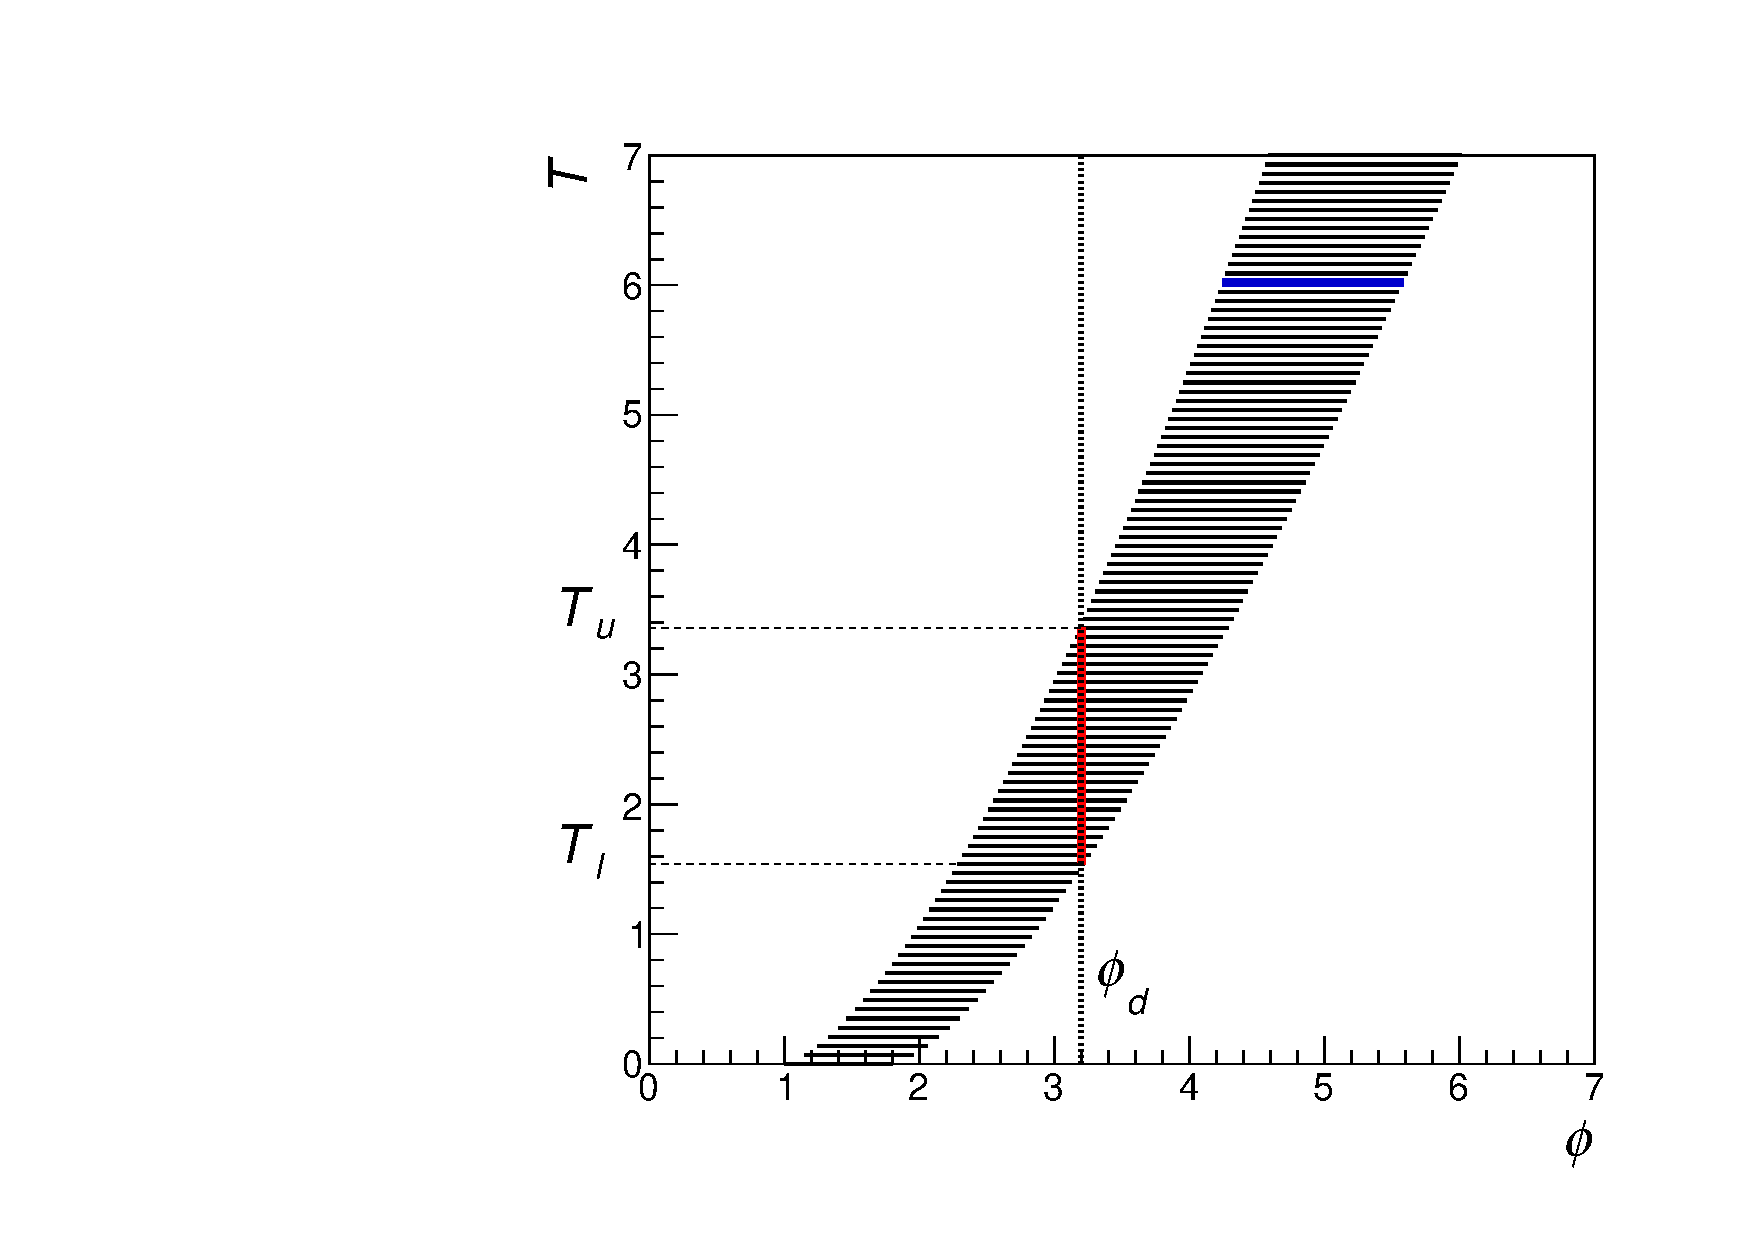
\includegraphics[width=0.6\textwidth]{figures/Intervals/neyman.pdf}
    \caption{302 The Neyman construction.  The horizontal bands gives likely values (at the 90\%
 level) of the test statistic $\phi$ (flux) for each value of the theory parameter $T$ (temperature).
 The  observed value of the test statistic $\phi_{d}$ is indicated by the vertical dotted line.
 This uses only the probability of different data, for given values of $T$;
 it does not involve probabilities of different values of $T$.
 A dotted vertical line at $\phi_{d}$ intersects
 the edges of the horizontal lines at $T_l$ and $T_u$, and these define the
 frequentist range for $T$ (indicated by the thick red vertical line). The value of $T=6$ in this case lies
 outside of the interval as the 90\% likely values of $\phi$ (indicated by the thick blue horizontal line) do not overlap with the observed value $\phi_{d}$. }
    \label{fig:neyman}
\end{figure}

In the Neyman construction, one must choose an ordering principle to select outcomes to include in the bands. In HEP (as detailed in Kendall and Stuart, and in the famous Feldman-Cousins paper \emph{"A Unified Approach to the Classical Statistical Analysis of Small Signals"}), the likelihood ratio is used to select the ``likely values'' to be included. In modern applications, this is particularly useful since it allows for a natural way to include nuisance parameters through the use of \emph{profiled} likelihoods. Moreover, often in HEP, rather than consider a sampled value $\phi$ as the test statistic and order using profile likelihood ratios, we can just use the profile likelihood ratio as the test statistic and as the ordering principle. This also very naturally extends to more than one parameter of interest. The procedure is as follows;
\begin{itemize}
    \item Define the test statistic using the profiled likelihood function $L$ as, 
    \begin{eqnarray}
        \zeta_{\mu} &= & \begin{cases}
               q(\mu,\hat{\eta}_{\mu})-q(\hat{\mu},\hat{\eta})    & \hat{\mu} \in \Omega \\
               q(\mu,\hat{\eta}_{\mu})-q(\hat{\mu}_{\Omega},\hat{\eta}_{\hat{\mu}_{\Omega}})            & \mathrm{else,}
                \end{cases}
    \end{eqnarray}
    where as usual $\mu$ are the parameters of interest bounded to $\mu\in\Omega$ and $\eta$ are the nuisance parameters, and $\hat{\mu}_{\Omega}$ means the value of $\mu$ that satisfies $\mathrm{max}\left\{q(\mu,\hat{\eta}_{\mu}):\mu\in\Omega\right\}$. 
    In the case of only one parameter of interest, the boundary condition can be expressed as $\mu\in[\mu_{a},\mu_{b}]$. 
    \item For each value of $\mu\in\Omega$ (representing the hypothesis $H(\mu)$), calculate $\zeta_{\mu}^{\mathrm{obs}}$ for the observed data and generate toy data (including for the constraint terms of any nuisance parameters, using their profiled values to define their probability density functions), to calculate the distribution $f(\zeta_{\mu}|H(\mu))$. 
    \item Choose a confidence level $(1-\alpha)$ and select the values of $\mu$ for which, 
    \begin{equation}
        p_{\mu}= \int_{\zeta_{\mu}^{\mathrm{obs}}}^{+\infty} f(\zeta_{\mu}|H(\mu)) d\zeta_{\mu} \geq \alpha.
    \end{equation}
    The union of all of these values forms the $100\times(1-\alpha)\%$ confidence region (interval for 1 parameter). Note that the ordering principle that we've used to calculate $p_{\mu}$ is the same as the Feldman-Cousins ordering rule (in the case of no nuisance parameters) and Kendall and Stuart (with nuisance parameters).  
\end{itemize}

\begin{tcolorbox}[colback=backblue]
\textbf{Example:} Let's go back to our example with the simple counting experiment, this time we'll determine the 68\% confidence interval on the parameter $\mu$, and keep the boundary on the parameter $\mu\geq0$, or in other words $\Omega = [0,+\infty)]$. A lot of the code can be repeated from when we were calculating the upper limit, however we need to change our test statistic as follows,
\begin{lstlisting}[style = Python]
# calculate test statistic
def zetamu(np,eta_p,mu):
  q_value        = q(mu,profiled_eta(mu,np,eta_p),np,eta_p)
  q_min,mu_min   = global_min(np,eta_p)
  if mu_min < 0 : return q_value-q(0,profiled_eta(0,np,eta_p),np,eta_p)
  else          : return q_value-q_min
\end{lstlisting}
and follow the procedure above. We loop over different values of $\mu$ and store the distributions using something like the code below, 
\begin{lstlisting}[style = Python]
import numpy
from model import *
from scipy.optimize import minimize
  
def global_min(np,eta_p):
  init_params = [0.1,-3.]
  bounds = [(-1,50),(-5,5)]
  # note q_constrained is the same function as q but 
  # with keyword arguments for the minimize function
  mle = minimize(q_unconstrained,\
        init_params,args=[np,eta_p],bounds=bounds)
  return mle.fun,mle.x[0]
  
mu_range   = numpy.arange(0,8,0.2)
zeta_range = numpy.arange(0,10,0.1)

# generate distribution f(zeta_mu) and find zeta_mu^68
def histo_zetamu(mu,zeta_obs):
  eta_profiled = profiled_eta(mu,n,0)
  ntoys = 10000
  toy_n   = numpy.random.poisson(lamb(mu,eta_profiled),size=ntoys)
  toy_eta = numpy.random.normal(eta_profiled,1,size=ntoys)
  zetamu_dist = [zetamu(np,eta_p,mu) for np,eta_p in zip(toy_n,toy_eta)]
  zetamu_dist.sort() ; zeta_68 = zetamu_dist[int(ntoys*0.68)]
  return zetamu_dist, zeta_68
 
# store the results as we go through the loop
zeta_obs_vals, zeta_68_vals = [], []
mu_interval, densities = [], []

# loop over mu values and see which ones pass the criteria
for mu_test in mu_range:
  zeta_obs = zetamu(n,0,mu_test)
  zetamu_toys,zeta_68 = histo_zetamu(mu_test,zeta_obs)
  density_vals = plt.hist(zetamu_toys,density=True,bins=zeta_range)
  densities.append(density_vals[0])
  zeta_68_vals.append(zeta_68)
  zeta_obs_vals.append(zeta_obs)
  if zeta_obs < zeta_68 : mu_interval.append(mu_test)
\end{lstlisting}

Figure~\ref{fig:neyman_counting} shows the distribution $f(\zeta_{\mu}|H(\mu))$ for fixed values of $\mu$. Also shown is the \emph{observed value} $\zeta^\mathrm{obs}_{\mu}$ -- unlike the solar temperature example, this is not a single number but of course depends on $\mu$. Finally, also plotted is the value of $\zeta_{\mu}$ (called $\zeta_{\mu}^{68}$) which is larger than 68\% of the toys in the distribution. This means that the values of $\mu$ to be included in the interval are those for which $\zeta^\mathrm{obs}_{\mu}< \zeta_{\mu}^{68}$. Keeping track of which $\mu$ values meet the criteria, the interval is be $0.50\leq\mu\leq6.20$. Note that we also know the maximum likelihood estimate of $\mu$ since its (by definition) the value of $\mu$ for which $\zeta_{\mu}=0$. Finally then we can say that our frequentist measurement is $\mu=2.22^{+3.98}_{-1.72}$.
%Note, to simplify things, I'm also going to stick to using the \textsf{scipy.optimize.minimize} function in my code.  
\end{tcolorbox}
\begin{figure}[hbt!]
    \centering
    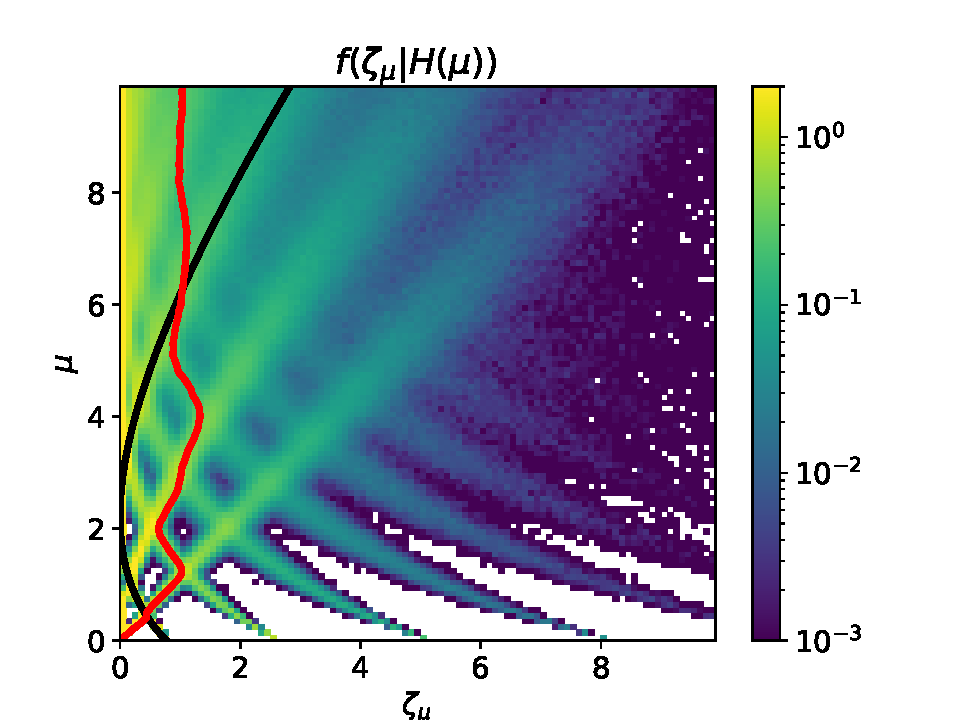
\includegraphics[width=\textwidth]{figures/Intervals/frequentist_interval.pdf}
    \caption{Distributions $f(\zeta_\mu|H(\mu))$ for different values of $\mu$ are shown by the color scale. The white regions show where there are no entries, highlighting the discrete nature of the Poisson probability distribution. The black like shows the observed values $\zeta_\mu^{\mathrm{obs}}$ and the red line shows $\zeta_{\mu}^{68}$ -- the value that 68\% of the distribution is smaller than. The values of $\mu$ for which $\zeta_\mu^{\mathrm{obs}} < \zeta_{\mu}^{68}$ form the 68\% confidence interval. }
    \label{fig:neyman_counting}
\end{figure}
In the counting experiment example, we saw that the region of $\zeta_{\mu}$ which contained 68\% of the toy data changed as a function of $\mu$, jumping around when $\mu\sim 0$. This is due to the discrete nature of the Poisson probability distribution and the effects of the boundary at $\mu=0$. However, for larger values of $\mu$, we see that this value seems to stay the same and becomes \emph{independent} of $\mu$. This is not so surprising given the law of large numbers since we know that as $\lambda\rightarrow \infty$, the Poisson distribution tends to a normal one. Furthermore, for \emph{any} likelihood function, the central limit theorem tells us that the likelihood estimator (which is a random value) should be distributed as a normal distribution. In the limit of large numbers then, there is no need to determine the $\zeta_{\mu}^{68}$ values using toys or even to determine the distribution at all with toys -- this is a convenient result (theorem) by \emph{Wilks'}. 

\subsection{Wilks' theorem and the MINOS method}
Wilks' theorem provides a very powerful result that allows us to calculate the distribution of $\zeta_{\mu}$, under certain conditions, in the limit of a large sample size. The most important of these conditions that particle physicists sometimes ignore is that the maximum likelihood estimate must not be at or beyond a boundary of the parameter space. In our counting experiment, this means that introducing the condition $\mu>0$, will have implications when the maximum likelihood estimate is close to 0. There are other conditions, but in HEP these are almost always satisfied so there's no need to cover them. 

Let's start with the simplest case where we have a single parameter of interest $\theta$ with no nuisance parameters. As usual, for $N$ observations of a random variable $X\sim f(X;\theta)$, we define, 
\begin{equation}
    \zeta_{N,\theta} = q_{N}(\theta)-q_{N}(\hat{\theta}) = -2\sum_{i=1}^{N}\ln f(X_{i};\theta) + 2\sum_{i=1}^{N}\ln f(X_{i};\hat{\theta}) .
\end{equation}
Providing that the derivatives of $f$ exist, we can Taylor expand the first derivative of $q_N$ to approximate the value at $\hat{\theta}$, 
\begin{equation}
   0= \frac{dq_{N}}{d\theta}\bigg|_{\theta=\hat{\theta}} = q_{N}'(\hat{\theta})  = q_{N}'(\theta)+q_{N}''(\theta) (\hat{\theta}-\theta),
\end{equation}
where the first equality is due to the fact that $\hat\theta$ is the value of $\theta$ that maximises the likelihood function $q_{N}$. We can re-write the equation as, 
\begin{equation}\label{eqn:randvarwt}
    (\hat{\theta}-\theta)\sqrt{q''_{N}(\theta)} = -\frac{q'_{N}(\theta)}{\sqrt{q''_{N}(\theta)}},
\end{equation}
which looks like an odd thing to do but it will be useful. Looking at the numerator on the RHS, we have, 
\begin{equation}
    -q'_{N}(\theta) = \frac{d}{d\theta}\sum_{i=1}^{N}2\ln f(X_{i};\theta)= \sum_{i=1}^{N} 2\frac{d}{d\theta}\left(\ln f(X_{i};\theta)\right).
\end{equation}
Now let's define the random variable $u=2\dfrac{d}{d\theta}\ln f(X|\theta)$, then we have that $-q'_{N}(\theta)$ looks like a sample mean of this random variable. In fact $-q'_{N}(\theta)=N\bar{u}$, where $\bar{u}$ is the sample mean of $u$. The expectation of $u$ can be found by considering that for any $\theta$,
\begin{eqnarray}
    1 &=& \int f(X;\theta)dX,                      \\
\end{eqnarray}
and therefore, taking derivatives,
\begin{eqnarray}
    0 &=& \frac{d}{d\theta} \int f(X;\theta)dX = \int \frac{d}{d\theta}  f(X;\theta)dX = \int \frac{d}{d\theta} \left(\ln f(X;\theta)\right)\cdot f(X;\theta)dX  \\ 
      &=& E\left[\frac{d}{d\theta}\ln f(X;\theta)\right]_{\theta} = \frac{1}{2}E\left[u\right]_{\theta},  
\end{eqnarray}
and hence the expectation of $u$ under $f(X;\theta)$ is 0. 
We can start to form a quantity $T_{N}$, given by, 
\begin{equation}
    T_{N,\theta} = \frac{N\bar{u} - NE[u]_{\theta}}{\sqrt{N\cdot V(u)_{\theta}}}
\end{equation}
We want to see what happens in the limit of $N\rightarrow\infty$, to the quantity $\sqrt{q''(\theta)}$. If its proportional to $\sqrt{N\cdot V(u)_{\theta}}$, then we have, by the central limit theorem, that $T_{\theta}$ (the limit of $T_{N,\theta}$) is distributed as $T_{\theta}\sim\phi(T_{\theta};0,1)$.

Let's take a look at $V(u)_{\theta}$. We have by definition that, \begin{eqnarray}
    V(u)_{\theta} & = &  E\left[(u-E[u]_{\theta})^{2}\right]_{\theta} = E\left[(u)^{2}\right]_{\theta} \\
     & = & 4\int \left(\frac{d}{d\theta}\ln f(X;\theta)\right)^{2}f(X;\theta)dX.
\end{eqnarray}
Recall again that, 
\begin{eqnarray}
    1 & = & \int f(X;\theta)dX
\end{eqnarray}
and differentiating twice we have, 
\begin{eqnarray}
    0 & = & \int \frac{d}{d\theta}\left(\frac{d}{d\theta}\ln f(x;\theta)\cdot f(X;\theta)\right)dX \\
     & = & \int \frac{d^2}{d\theta^2}\ln f(X;\theta) \cdot f(X;\theta)dX +  \int \frac{d}{d\theta}\ln f(X;\theta) \cdot \frac{d}{d\theta}f(X;\theta)dX  \\
     & = & \int \frac{d^2}{d\theta^2}\ln f(X;\theta) \cdot f(X;\theta)dX +  \int \frac{d}{d\theta}\ln f(X;\theta) \cdot \frac{d}{d\theta}\ln f(X;\theta)\cdot f(X;\theta) dX\\ 
     & = & \int \frac{d^2}{d\theta^2}\ln f(X;\theta) \cdot f(X;\theta)dX +  \int \left(\frac{d}{d\theta}\ln f(X;\theta) \right)^{2} f(X;\theta) dX \\
     & = & \int \frac{d^2}{d\theta^2}\ln f(X;\theta) \cdot f(X;\theta)dX +  \frac{1}{4}V(u)_{\theta}, 
\end{eqnarray}
so that, 
\begin{eqnarray}
\frac{1}{4}V(u)_{\theta} = - \int \frac{d^2}{d\theta^2}\ln f(X;\theta) \cdot f(X;\theta)dX = - E\left[\frac{d^{2}}{d\theta^{2}}\ln f(X;\theta)\right]_{\theta}.
\end{eqnarray}
But remember that $q''_{N}(\theta) = -2 \sum_{i=1}^{N} \dfrac{d^2}{d\theta^2}\ln f(X;\theta)$. By the law of large numbers, we must have that $\dfrac{-q''_{N}(\theta)}{N}\rightarrow 2E\left[\dfrac{d^2}{d\theta^2}\ln f(X;\theta)\right]_{\theta}$ as $N\rightarrow \infty$. But this is just $-\dfrac{1}{2}V(u)_{\theta}$! So then we have $\dfrac{q''_{N}(\theta)}{N}\rightarrow  \dfrac{1}{2}V(u)_{\theta}$.
Now (in a rather hand-wavy fashion), we can say that,
\begin{eqnarray}\label{eqn:part1}
  \frac{1}{\sqrt{2}}(\hat{\theta}-\theta)\sqrt{q''_{N}(\theta)}  = -\frac{q'_{N}(\theta)}{\sqrt{2 q''_{N}(\theta)}} \rightarrow 
\frac{q'_{N}(\theta)}{\sqrt{N\cdot V(u)_{\theta} }} = \frac{N\bar{u}-NE[u]_{\theta}}{\sqrt{N\cdot V(u)_{\theta} }} = T_{N,\theta} \rightarrow T_{\theta}\sim\phi(T_{\theta};0,1).
\end{eqnarray}
We've been a bit careless here since the numerator converges in distribution and the denominator converges in probability, and we've performed the two limits separately. However, but there is a theorem (which we won't go into) for ratios of such random variables, numerator converging in distribution and denominator in probability, due to Slutsky which yields the same result so in the end its ok.  

Let's go back to the definition of $\zeta_{N,\theta}.$ Again, we take a Taylor expansion, this time of the function $q_{N}(\theta)$,
\begin{equation}\label{eqn:taylor_exp_qN}
    q_{N}(\theta) = q(\hat\theta) + \cancelto{0}{q'_{N}(\hat{\theta})}(\theta-\hat{\theta}) + \frac{1}{2}q''_{N}(\hat\theta)(\theta-\hat{\theta})^2,
\end{equation}
and so, 
\begin{equation}\label{eqn:part2}
    \zeta_{N,\theta} =  \frac{1}{2}q''_{N}(\hat\theta)(\theta-\hat{\theta})^2 = \left( \frac{1}{\sqrt{2}}(\hat{\theta}-{\theta})\sqrt{q''_{N}(\hat\theta)}\right)^2. 
\end{equation}
Now the term inside the square on the RHS of Eqn~\ref{eqn:part2} is the same as in the LHS of Eqn.~\ref{eqn:part1}, except for the value of $\theta$ at which the second derivative is evaluated. However, since the maximum likelihood estimate is \emph{consistent}, $\hat\theta\rightarrow \theta_{0}$ as $N\rightarrow \infty$. So in the limit $N\rightarrow \infty$, we replace $\theta$ with $\theta_{0}$, and study the distribution of $\zeta_{\theta}$ for the true value of $\theta=\theta_{0}$. In this limit we can then equate the LHS of Eqn.~\ref{eqn:part1} with the term inside the square, so that, 
\begin{equation}
    \zeta_{N,\theta_0} = (T_{N,\theta_{0}})^2.
\end{equation}
But we know that $T_{N,\theta_0}$ is distributed as a unit normal $\phi(T;0,1)$ under the hypothesis $H(\theta_0)$ \emph{for any value of $\theta$} as $N\rightarrow \infty$ so we can also figure out the distribution of $(T_{N,\theta_{0}})^2$. This distribution is known as a $\chi^{2}$ -- a \emph{chi-square} distribution with 1 degree of freedom. It has the probability density function, 
\begin{equation}
    \chi^{2}(X;1) = \frac{1}{\sqrt{2\pi X}}e^{-\frac{X}{2}}.
\end{equation}
This is the result of Wilks' theorem for one parameter. In general, Wilks' theorem gives us the result for any number of degrees of freedom. The result is that for a log-likelihood difference with $n$ parameters $\theta_{1},\theta_{2},...,\theta_{n}$, the test statistic $\zeta_{\theta_{1},...,\theta_{n}}$ will be distributed under $H(\theta_{1},...,\theta_{n})$ (the null hypothesis) as, 
\begin{equation}
  f(\zeta_{\theta_{1},...,\theta_{n}}|H(\theta_{1},...,\theta_{n})) = \chi^{2}(\zeta_{\theta_{1},...,\theta_{n}};n),
\end{equation}
where $\chi^{2}(\cdot;n)$ is the chi-square distribution with $n$ degrees of freedom, in the limit of large sample sizes. 
If we know the distribution of $\zeta$, then we can calculate $p_{\theta}$ for any value of $\zeta_{\theta}$ by looking up the cumulative distribution function of the $\chi^2$ functions. Moreover, the value of $\zeta^{68}_\theta$ (and any quantile, not just the 68\% one) is independent of $\theta$!. Any one of your favourite statistics programming languages will be able to calculate this for you, for example in python, we can use the \textsf{scipy.stats.chi2} class and use the \textsf{chi2.cdf} function. Figure~\ref{fig:chisquare} shows the probability density and cumulative density functions for the $\chi^{2}$ with increasing numbers of degrees of freedom. Using the cumulative distribution, it is possible to read off $p-$values or the value of $X$ that would contain some percentage of the distribution. 
\begin{figure}[hbt!]
    \centering
    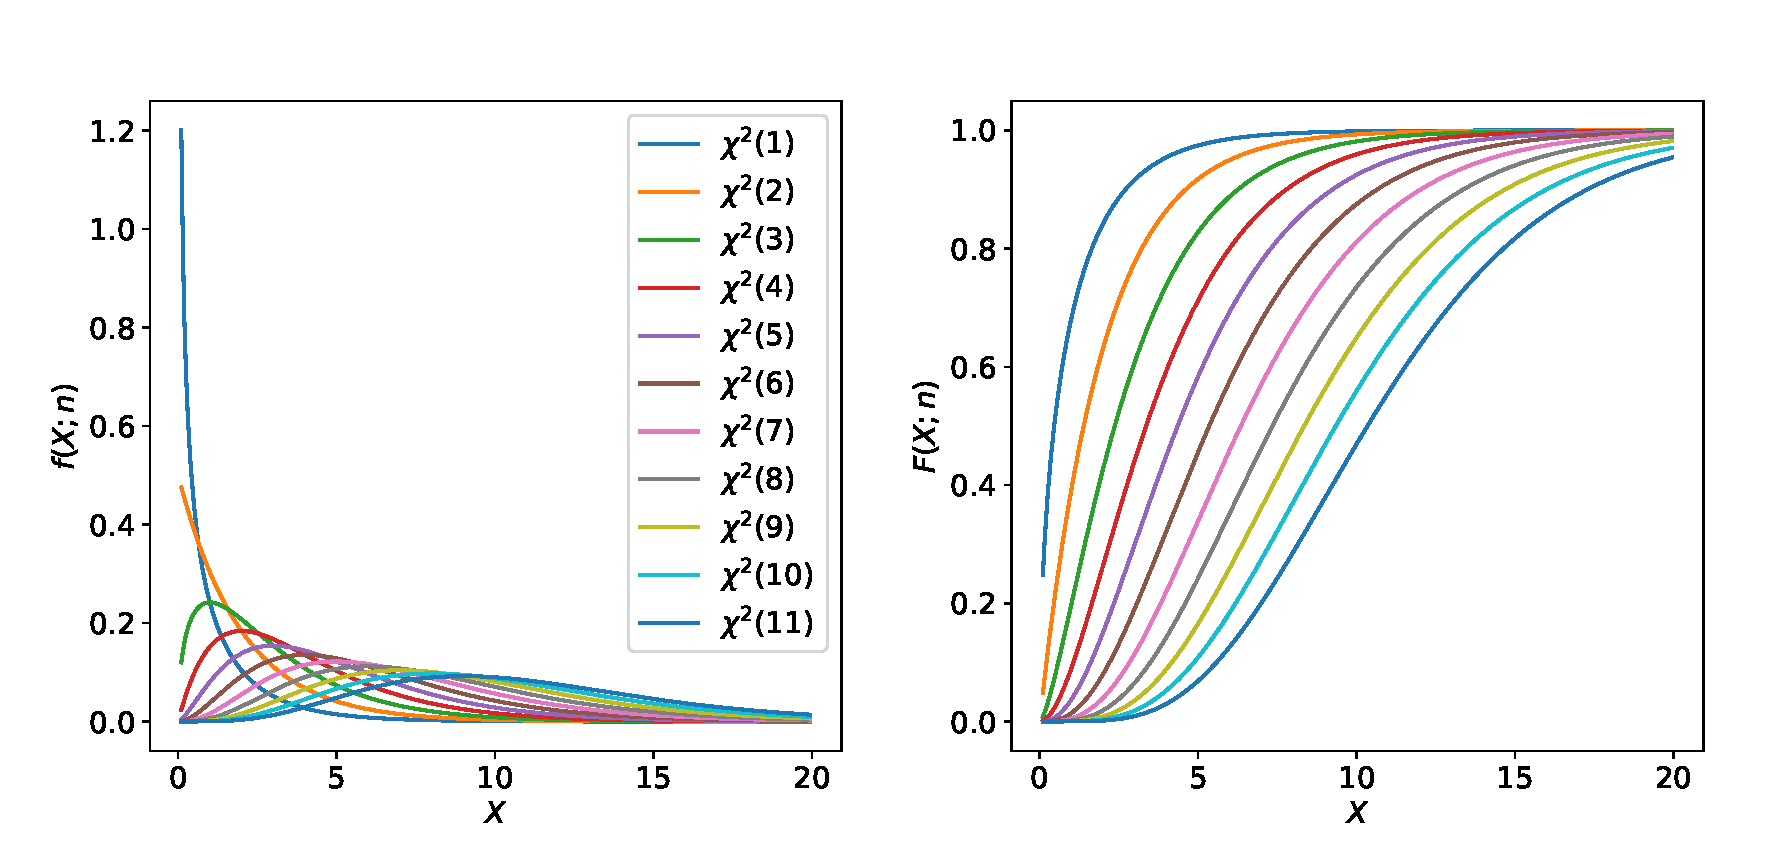
\includegraphics[width=\textwidth]{figures/Intervals/chi2dists.pdf}
    \caption{Probability density (left) and cumulative density (right) functions for the $\chi^{2}$ with increasing numbers of degrees of freedom.}
    \label{fig:chisquare}
\end{figure}
Calculating intervals or confidence regions for parameters becomes straightforward since for each value, we know the distribution of $\zeta_{\theta}$ under the hypothesis $H(\theta)$ simply by knowing the dimension of $\theta$ and calculating $\zeta_{\theta}^{\mathrm{obs}}$. The $(1-\alpha)$ confidence region in $n-$dimensions is determined by the values of $\theta$ for which,
\begin{equation}
    \zeta_{\theta}^{\mathrm{obs}}=q(\theta)-q(\hat{\theta})=
    \Delta q(\theta) \leq Q
\end{equation}
where $\int_{Q}^{+\infty} \chi^{2}(\zeta_{\theta};n)d\zeta_{\theta} = \alpha$. For example, if $n=1$ and $(1-\alpha)=0.683$, then  $Q=1$, while if $n=1$ and $(1-\alpha)=0.954$, then $Q=4$. In our goodness of fit test, we could have used this result to calculate the $p-$value and our number of degrees of freedom would be the number of bins. 

Let's look at an example of trying to measure two signal rates over a falling background distribution, using a binned likelihood. We'll include nuisance parameters, but remember that we don't include them in the definition of the test-statistic -- they are profiled.  

\begin{tcolorbox}[colback=backblue]
\textbf{Example:} We have an analysis in which the number of events in bins of a distribution is counted. There is a background process and two signal processes with signal strength modifiers $\mu_1$ and $\mu_2$, with no restrictions on their range. Our log-likelihood function for this will be, 
\begin{equation}
    q(\mu_1,\mu_2,\eta) = -2 \left(\sum_{i} n\ln{\lambda_{i}}- \lambda_{i} \right) + \eta^{2},
\end{equation}
where $i$ runs over the bins, $\lambda_{i}=\mu_{1}s_{i,1}+\mu_{2}s_{i,2}+b_{i}(1+k_{i})^{\eta}$,
and $\eta$ is a nuisance parameter which can change the slope of the background (due to the $\kappa_{i}$ being different for each bin. 
The model can is defined using the snippet below, 
\begin{lstlisting}[style = Python]
signal1_counts=[0,0,0,0.5,1,2,3,4,5,4.5,4.0,3.5,3.0,2.5,2,\ 
    1.5,1,0.5,0,0,0,0,0,0,0]
    
signal2_counts=[0,0,1,2,3,4,5,6,5,3,1,0,0,0,0,0,\ 
    0,0,0,0,0,0,0,0,0]
    
background_counts=[60*numpy.exp(-0.1*i) \
    for i in range(len(signal1_counts))]
    
bkg_uncert=[0.3,0.3,0.3,0.2,0.2,0.2,0.2,0.2,0.2,0.1,0.1,0.1,\
    0.1,0.1,0.1,0.1,0.1,0.05, 0.05,0.05,0.05,0.02,0.02,0.02,0.02]
    
nbins = len(signal1_counts)

def lamb(i,mu1,mu2,eta):
  s1 = signal1_counts[i]
  s2 = signal2_counts[i]
  b = background_counts[i]
  k = bkg_uncert[i]
  return mu1*s1+mu2*s2+b*(1+k)**eta

data=[65,45,47,37,37,40,42,36,34,36,22,23,23,18,\ 
    17,13,12,12,11,12,6,6,6,9,4]
\end{lstlisting}
Figure~\ref{fig:example_binneddata} shows the background and signal distributions at the global minimum $(\hat{\mu}_{1},\hat{\mu}_{2},\hat{\eta})$. The data is shown on top with each data point indicating the standard deviation of a Poisson distribution with the same mean as the observed data in that bin. We scan the value of, 
\begin{equation}
    \Delta q(\mu_1,\mu_2) =  q(\mu_1,\mu_2,\hat{\eta}_{\mu_1,\mu_2}) - q(\hat{\mu}_1,\hat{\mu}_2,\hat{\eta}).
\end{equation}
Figure~\ref{fig:example_binnedlh} shows the value using a color scale. Using Wilks' theorem, the 68.3\% and 95.4\% confidence regions are the regions for which $ \Delta q(\mu_1,\mu_2) < 2.3$ and  $ \Delta q(\mu_1,\mu_2) < 5.99$ respectively, as indicated by the contours. If we are interested in only the first parameter, $\mu_1$, then we can use the function,  
\begin{equation}
    \Delta q(\mu_1) =  q(\mu_1,\hat{\mu}_{2,mu_{1}},\hat{\eta}_{\mu_1}) - q(\hat{\mu}_1,\hat{\mu}_2,\hat{\eta}).
\end{equation} 
The 68.3\% and 95.4\% intervals are found as the region for which  $\Delta q(\mu_1)<1$ and $\Delta q(\mu_1)<4$, respectively. We can find these intersections using some code similar to that below, 
\begin{lstlisting}[style = Python]
def findIntervals(x,y,conts=[1,4]):
  xx0,yy0 = x[0],y[0]
  crossing_x = []
  for xx,yy in zip(x[1:],y[1:]):
    for K in conts:
      if (yy < K and yy0 > K) or (yy > K and yy0 < K):
        crossing_x.append(return_crossing(xx0,yy0,xx,yy,K))
    xx0=xx
    yy0=yy
  return crossing_x

mu1_axis = numpy.linspace(-1,5,50)
z = [ delta_qmu1(data,m1,q_min) for m1 in mu1_axis]
intervals = findIntervals(mu1_axis,z,[1,4])
\end{lstlisting}
The function $\Delta q(\mu_1)$ and intervals are shown in Figure~\ref{fig:example_binnedlh}. If we didn't profile $\mu_{2}$, the intervals would be smaller, which shows the effect of correlations between parameters of interest. 
\end{tcolorbox}
\begin{figure}
    \centering
     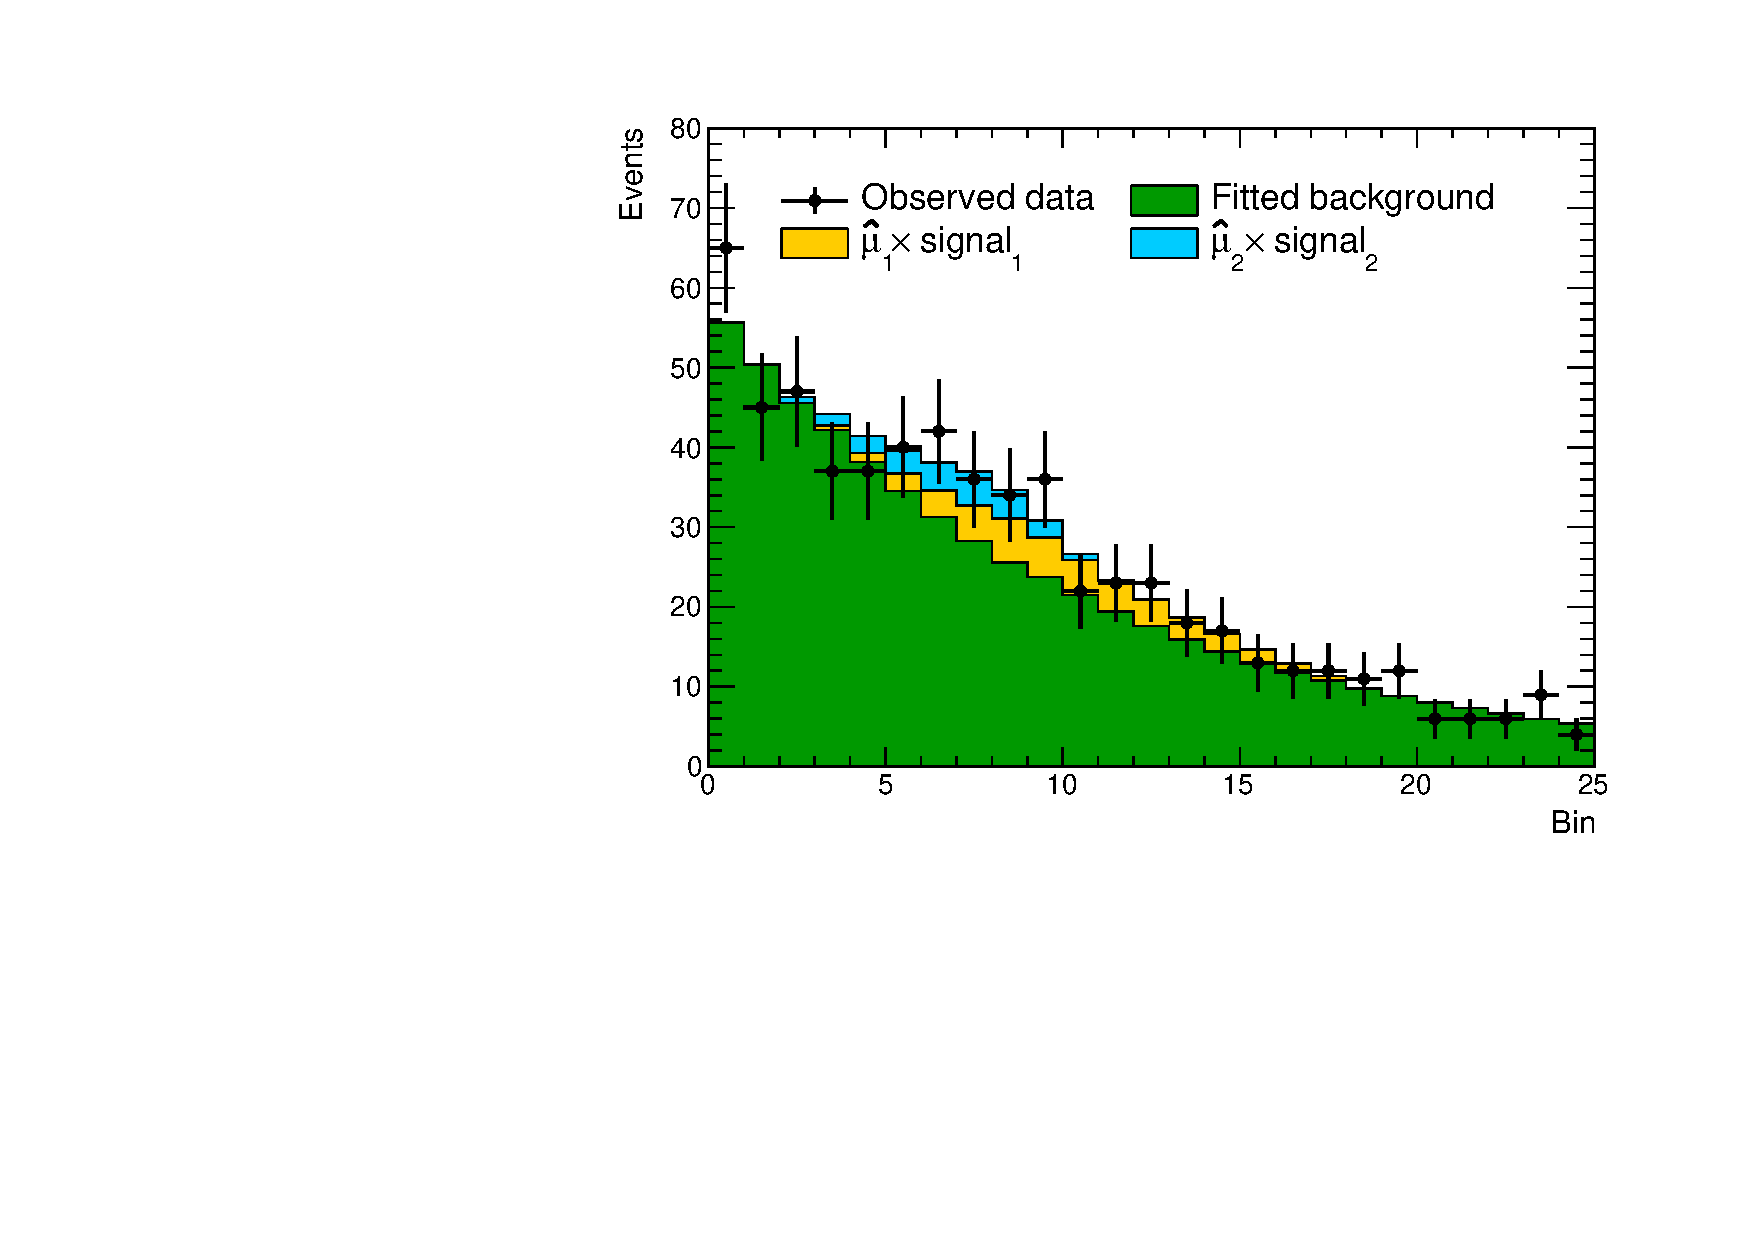
\includegraphics[width=0.8\textwidth]{figures/Intervals/data_model_plot.pdf}
    \caption{Background and signal distributions at the global minimum of the likelihood parameters, stacked on top of one another. The data is shown too, and the error bars represent the standard deviation of a Poisson with the same mean. }
    \label{fig:example_binneddata}
\end{figure}

\begin{figure}[hbt!]
    \centering
    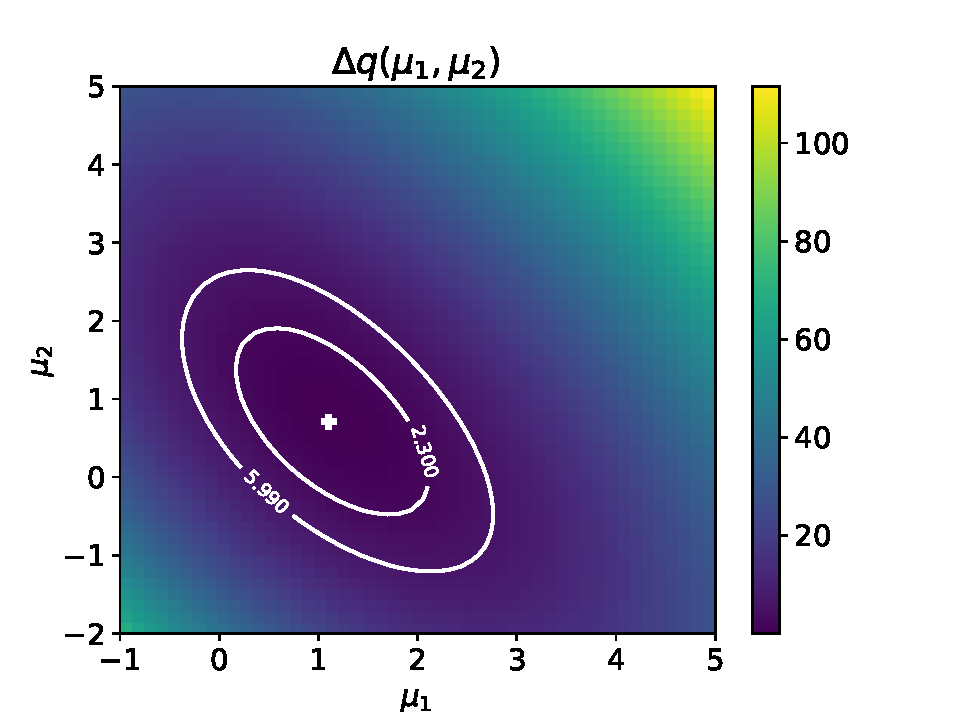
\includegraphics[width=0.49\textwidth]{figures/Intervals/likelihood_scan_mu1_mu2.pdf}
    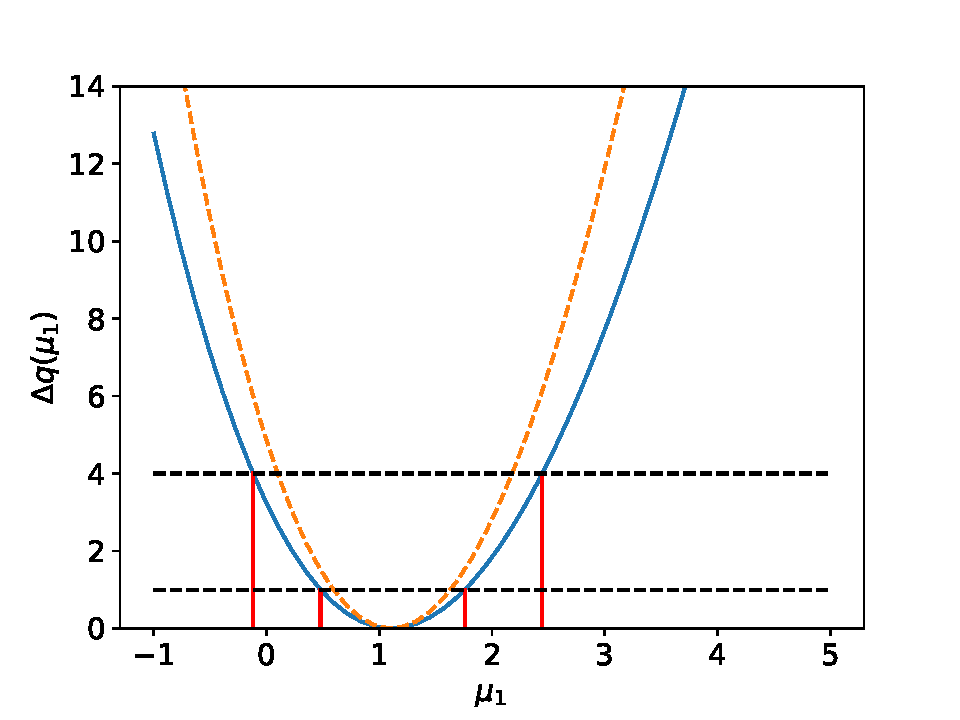
\includegraphics[width=0.49\textwidth]{figures/Intervals/scan_mu1.pdf}
    \caption{Left: $\Delta q(\mu_1,\mu_2)$ in color scale and contours corresponding to the boundaries of the 68.3\% and 95.4\% confidence regions. Right: $\Delta q(\mu_1)$ both profiling (blue line) and fixing $\mu_{2}$ (orange dashed line) the 68.3\% and 95.4\% confidence intervals are indicated by the red lines.   }
    \label{fig:example_binnedlh}
\end{figure}
Extracting the intervals/regions this way (using the profiled log-likelihood) is often referred to as the \textsf{MINOS} method (as this is the method used in the  \textsf{MINOS} code to determine uncertainties). 
 
Remember that in our definition of $\zeta_{\mu}$ for the simple counting experiment, we had two clauses depending on whether or not the signal strength ($\mu$) was greater than 0 or not. The introduction of this boundary poses no problem when constructing the frequentist intervals, however, it will have an effect when appealing to Wilks' theorem, as the assumption that $\zeta_{\mu}$ is distributed as a $\chi^{2}(2)$ will breakdown when $\mu\sim 0$. Figure~\ref{fig:example_fc} shows an example of this happening in a CMS analysis of Higgs boson decays to $\gamma\gamma$ with the Run-1 dataset. The parameters $\mu_{\mathrm{ggH+ttH}}$ and  $\mu_{\mathrm{VH+qqH}}$ are signal strengths for Higgs boson production modes involving fermion and vector-boson couplings, respectively. In this model, these parameters are bounded to be $>0$. The contours indicate the 68\% and 95\% confidence regions determined from the observed data using a Neyman construction with likelihood ratio ordering (labelled ``Feldman-Cousins'') and appealing to Wilks' theorem (labelled ``Likelihood Scan''). Away from the boundaries, the contours agree rather well -- meaning that the conditions for Wilks' theorem to apply hold. However, close to the boundaries, the contours start to disagree. This is not due to there being not enough events in the sample, but really a consequence of the boundary. It is therefore important to check the coverage of the intervals/regions reported when using the \textsf{MINOS} method, when there are boundaries in the problem. 
\begin{figure}[hbt!]
    \centering
    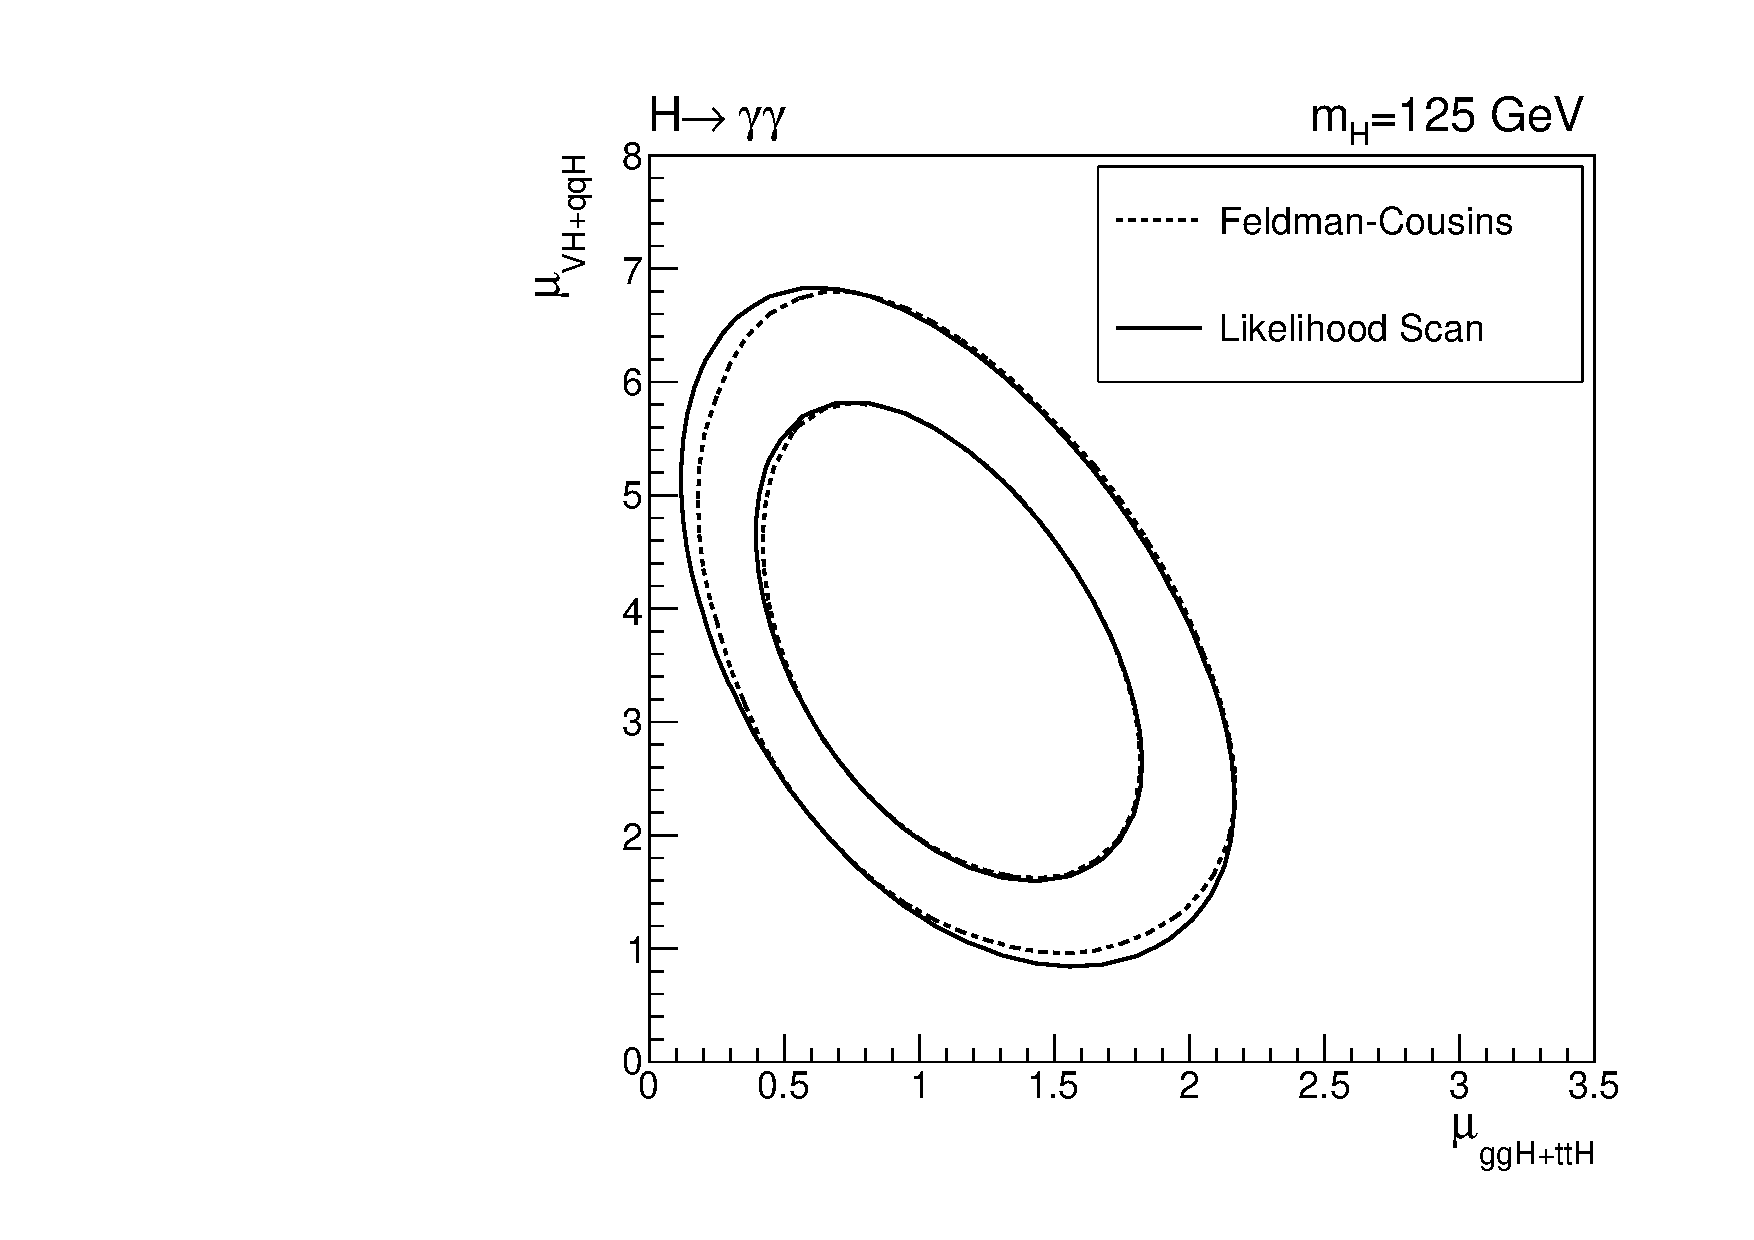
\includegraphics[width=0.6\textwidth]{figures/Intervals/compare-fc-lh.pdf}
    \caption{CMS analysis of Higgs boson decays to $\gamma\gamma$ with the Run-1 dataset. The two parameters are bounded to be $>0$. The contours indicate the 68\% and 95\% confidence regions determined from the observed data using a Neyman construction with likelihood ratio ordering (labelled ``Feldman-Cousins'') and appealing to Wilks' theorem (labelled ``Likelihood Scan'').}
    \label{fig:example_fc}
\end{figure}

\textcolor{red}{Add here something about the Hessian approach for approximating uncertainties, since this thing is gaussian near the minimum.}

Note that we can even go one step further in approximation. Let's go back to equation~\ref{eqn:taylor_exp_qN}. We can see that in 1-dimension, this is just a parabolic function. Re-arranging gives us the usual approximation,

\begin{equation}\label{eqn:hessianderive1d}
    2(q_{N}(\theta)-q(\hat{\theta})) = q''_{N}(\hat{\theta})(\theta-\hat{\theta})^{2}
\end{equation}

i.e twice the difference in the negative log-likelihood to the value at the minimum looks like a parabola, close to the minimum, that is centered at $\hat{\theta}$. If we had a random variable that was distributed as a Gaussian with $\theta\sim \phi(\hat{\theta},\sigma)$, we would find that that the twice the negative log-likelihood would be, 

\begin{equation}
-2\left(\ln(\phi(\theta,\sigma)) - \ln(\phi(\hat{\theta},\sigma)) \right)
= -2\left( \frac{1}{2}\left(\frac{\theta-\hat{\theta}}{\sigma}\right)^{2} - \frac{1}{2}\left(\frac{\hat{\theta}-\hat{\theta}}{\sigma}\right)^2\right)  
= \left(\frac{\theta-\hat{\theta}}{\sigma}\right)^{2},
\end{equation}

where constant terms cancel in the second step. This means if we match with equation~\ref{eqn:hessianderive1d}, we can clearly see that,

\begin{equation}
\frac{1}{\sigma^{2}} = q''_{N}(\hat{\theta}).
\end{equation}

So in this approximation, since for a Gaussian distribution, the 68.3\% interval is given by the standard deviation, our 68.3\% is given by the 2nd derivative of twice the difference in the negative log-likelihood function, evaluated at the minimum. This result extends to more than one dimension simply replacing $q''_{N}$ with the Hessian yields an approximation of the  co-variance matrix in multi-dimensional fits. However, often its better to use the method previously described finding the intervals via the crossings at set levels to determine confidence intervals, so we won't use this method further.  

\subsection{Coverage in the counting experiment}

Now let's return to our simple counting experiment. Close to the boundary $\mu=0$, we have two issues with applying Wilks' theorem. The first is not being in the limit of large $N$ and the second being the boundary itself. We can check what the coverage of the method (say for the 68.3\% interval) by determining the \emph{fraction of intervals} in $\mu$, as a function of the true value $\mu_0$, that contain $\mu_{0}$. It sounds like a rather painful ordeal given that calculating a single interval can take time, however, we do not need to calculate each interval to figure out the coverage. Remember that $\mu$ is included in the interval provided $\zeta^{\mathrm{obs}}_{\mu}\leq\zeta^{68.3}_{\mu}$. For the Neyman construction, we can use toys to calculate $\zeta^{68.3}_{\mu}$, while for the \textsf{MINOS} method, we assume $\zeta^{68.3}_{\mu}=1$. Figure~\ref{fig:coverage} shows the coverage in $\mu$ when calculating the intervals using the Neyman construction and using the \textsf{MINOS} method for our counting experiment.  
\begin{figure}[hbt!]
    \centering
    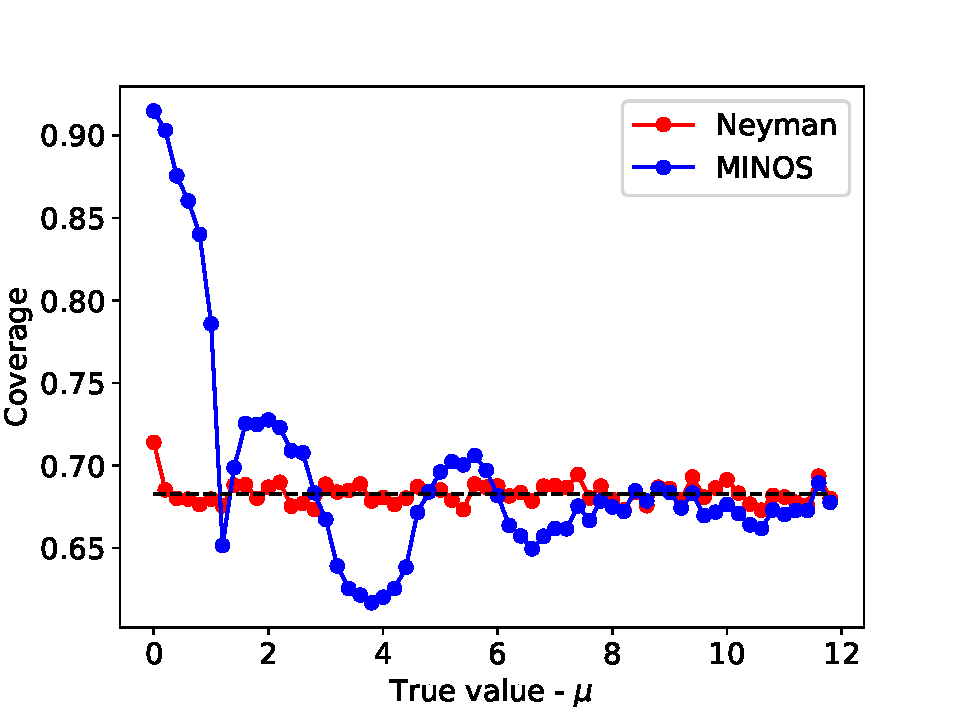
\includegraphics{figures/Intervals/coverage_example.pdf}
    \caption{Coverage of intervals in $\mu$ for the counting experiment, when calculated using the Neyman construction compared to the \textsf{MINOS} method, as a function of the true value $\mu$.}
    \label{fig:coverage}
\end{figure}
You can see that the Neyman construction gives very close coverage to the desired 68.3\% except at very small $\mu$, where the discrete nature of the Poisson distribution makes it difficult to find the exact $\zeta^{68.3}_{\mu}$ -- in fact this is still seen at larger values, though the effect gets reduced. Instead, the \textsf{MINOS} method, jumps between over-coverage and undercoverage, eventually settling down only above $\mu\sim 8$. This is not surprising since the distribution of $\zeta_{\mu}$ really doesn't look like a $\chi^{2}(1)$. Figure~\ref{fig:chisquare_zetamu} shows the distribution of $\zeta_{\mu}$ at $\mu=0.1$ and $\mu=9$. For the larger value, away from the boundary the approximation of a $\chi^{2}(1)$ is much more accurate. 
\begin{figure}
    \centering
    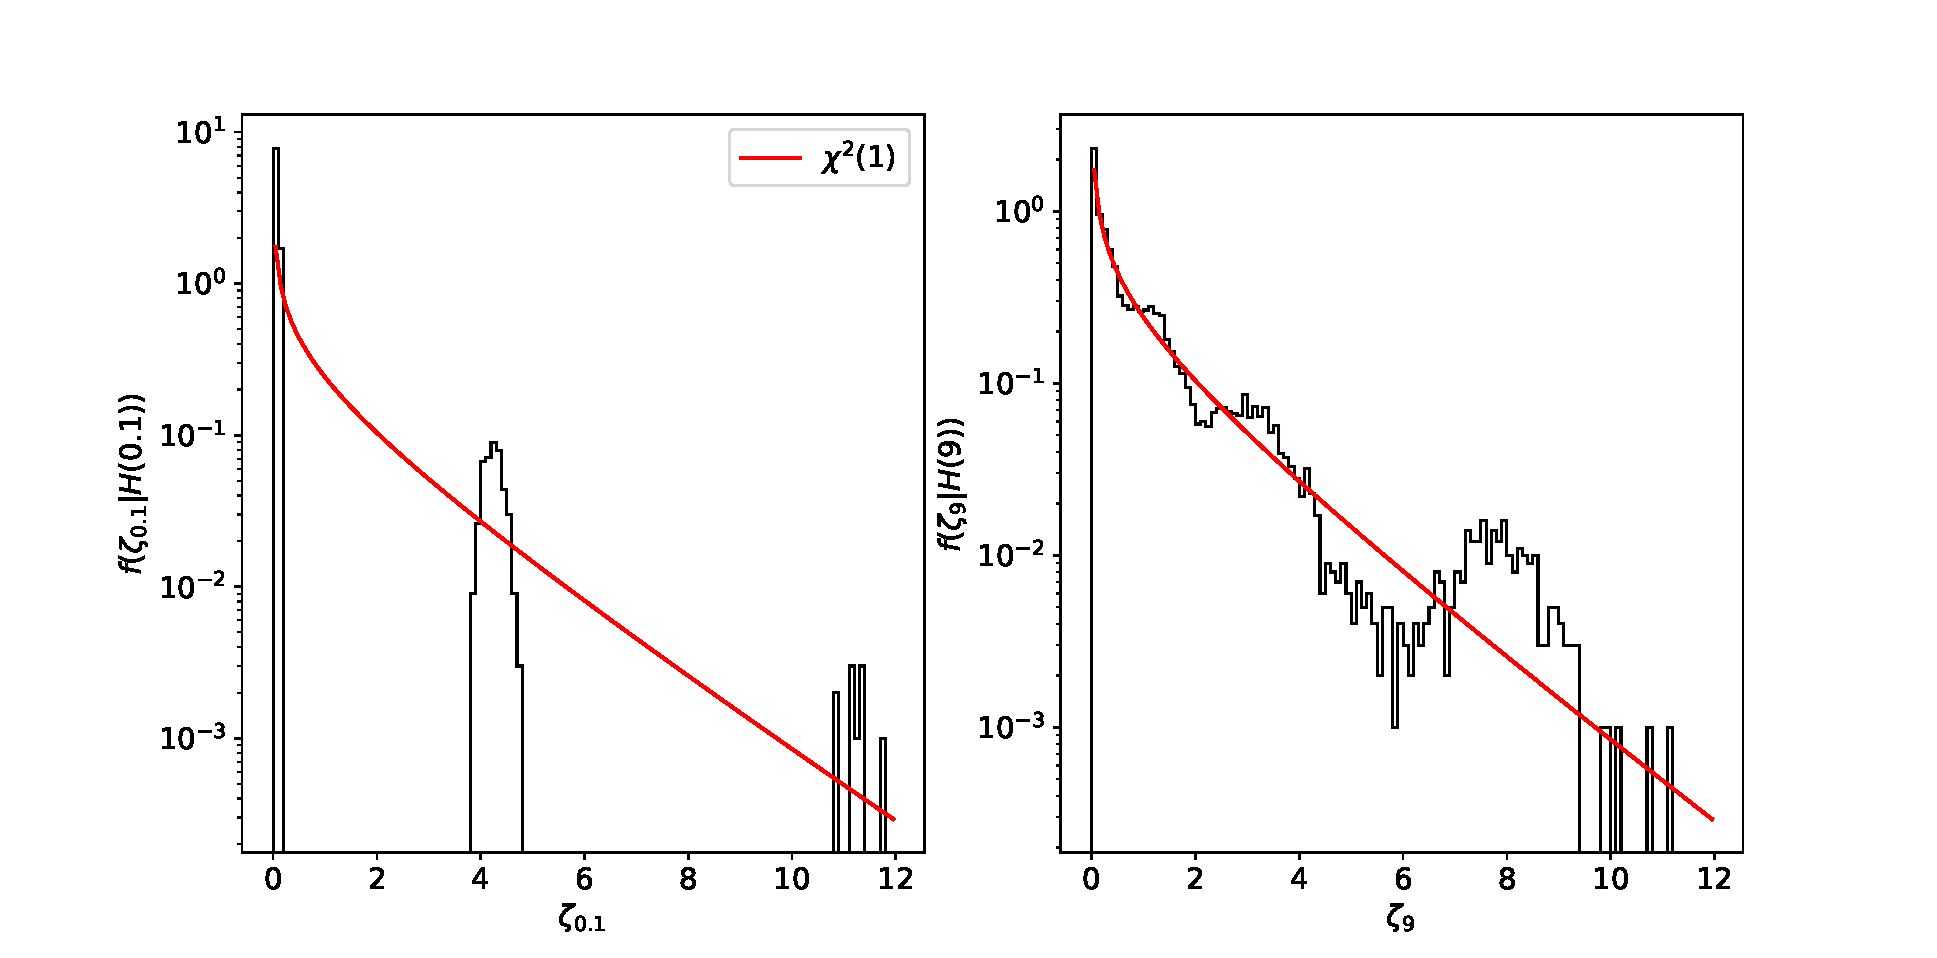
\includegraphics[width=\textwidth]{figures/Intervals/tmu_dists_example.pdf}
    \caption{Distribution of $\zeta_{\mu}$ for $\mu=0.1$ (left) and $\mu=9$, for the counting experiment, with a boundary $\mu>0$. The black histograms are the real distribution, evaluated using toys, while the red like is the approximate distribution using Wilks' theorem.}
    \label{fig:chisquare_zetamu}
\end{figure}

\subsection{Conversions to Z-scores}
The $\chi^{2}$ distribution is often used to provide a simple conversion from $p$-values (which can get very small) to more reasonable numbers. In HEP, you'll find that physicists thend to convert an observed $p$-value ($p$) into an equivalent ``\emph{number of sigma'' $n(\sigma)$} or Z-score for a normal distribution using, 
\begin{eqnarray}
    p & = &  \int_{Q}^{+\infty}\chi^{2}(X;1)dX \\
    \mathrm{Z}& = & \sqrt{Q}
\end{eqnarray} 
It should be noted that this is \emph{only a conversion convention} and doesn't tell us anything about the underlying distributions or the number of degrees of freedom. The conversion is always done using a $\chi^{2}(1)$. Eg, when a particle physicist talks about ``a more than 3$\sigma$ discrepancy'', they always mean that the $p-$value of the test under the null is smaller than $\int_{3^{2}}^{\infty}\chi^{2}(X;1)dX$. 

Often, particle physicists will refer to a \emph{1-sided} test, in which case the conversion is performed using the following, 
\begin{eqnarray}\label{eqn:convertpval}
    p & = & \int_{Q}^{+\infty}\left(\frac{1}{2}\delta(0)+\frac{1}{2}\chi^{2}(X;1)\right)dX \\
    \mathrm{Z}& = & \sqrt{Q}
\end{eqnarray} 
Usually this is the case when talking about ``discovery'' of a new process. For example, the test statistic used in the Higgs boson discovery (and in many results since), was, 
\begin{equation}
    t_{0} = \begin{cases}
                q(0,\hat{\eta}_{0})-q(\hat{\mu},\hat{\eta})    & \hat{\mu} > 0 \\
                0               & \hat{\mu}\leq 0,
                \end{cases}
\end{equation}
where $\mu$ is an overall signal rate multiplier, and we are interested in rejecting the hypothesis $\mu=0$ -- $H(0)$. It can be shown that in the limit of large numbers, $f(t_{0}|H(0)) = \frac{1}{2}\delta(0)+\frac{1}{2}\chi^{2}(t_0;1)$, meaning the $p$-value ($p_{0})$ can be calculated using Eqn~\ref{eqn:convertpval}, and the Z-score is $\sqrt{t^{\mathrm{obs}}_{0}}$. Particle physicists get excited when $t_{0}^{\mathrm{obs}}>25$ -- which corresponds to the ``5 sigma discovery''. I personally think this all adds more confusion than clarification and the best practise is to explain the hypotheses being performed and the criteria to reject or accept hypotheses. 

\subsection{Bayesian credible intervals}
As a last remark, we should return to the Bayesian's answer for what $X\pm\sigma_{X}$ means. It's a lot more simple than the freqeuntist answer, but remember that the interpretation is quite different. Once the posterior distribution $P(\mu)$ is obtained (by marginalising over the nuisance parameters $\eta$, a Bayesian can quote a $(100\times\alpha)$\% \emph{credible interval} (or credible region in more than one dimension), as a region $\mu\in\Omega_{\alpha}$ for which,
\begin{equation}\label{eqn:credible}
    P(\mu\in\Omega_{\alpha})=\int_{\Omega_{\alpha}} P(\mu)d\mu = \alpha.
\end{equation}
Its as simple as that right? Not quite! There can be multiple such regions, any of which satisfy Eqn.~\ref{eqn:credible}. It's best to show the posterior distribution in publications, and describe any interval that is quoted as a result. Below is a snippet of python code that calculates the \emph{shortest} 68.3\% interval for our countin experiment. Note that many of the functions were already defined in Section~\ref{sec:marginalised}, so I won't bother repeating them.
\begin{lstlisting}[style = Python]
import marginalised_likelihood

# new prior on mu P(mu)
def prior_mu_new(mu):
  if (mu > 50 or mu < 0) : return 0
  else: return 1./50

marginalised_likelihood.prior_mu = prior_mu_new

marginalised_likelihood.prior_mu = prior_mu_new
xaxis = numpy.linspace(-1,20,5000)
normalisation = marginalised_likelihood.norm(n)
posterior_dist = [ marginalised_likelihood.integral(n,mu)/normalisation \
for mu in xaxis ]

# use an approximate for the integral with rectangles
intervals=[]
for i in range(len(xaxis)):
 x = xaxis[i]
 if x > 5: break
 inte=0
 for j in range(i,len(xaxis)-1):
   y = xaxis[j+1]
   yl = xaxis[j]
   inte += posterior_dist[j]*(y-yl)
   if inte >= 0.683:
    intervals.append([y-x,[x,y],[i,j]])
    break

# find the shortest one
intervals.sort(); interval = intervals[0]
print("68.3%% interval (%.2f,%.2f)"%(interval[1][0],interval[1][1]))
\end{lstlisting}

Figure~\ref{fig:posterior_shortest_interval} shows the posterior distribution $P(\mu)$ for the counting experiment, this time restricting $\mu>0$ by setting the prior $\pi(\mu)=0$ for $\mu\leq0$. The shaded region indicates the shortest 68.3\% credible interval for $\mu$. 

\begin{figure}[hbt!]
    \centering
    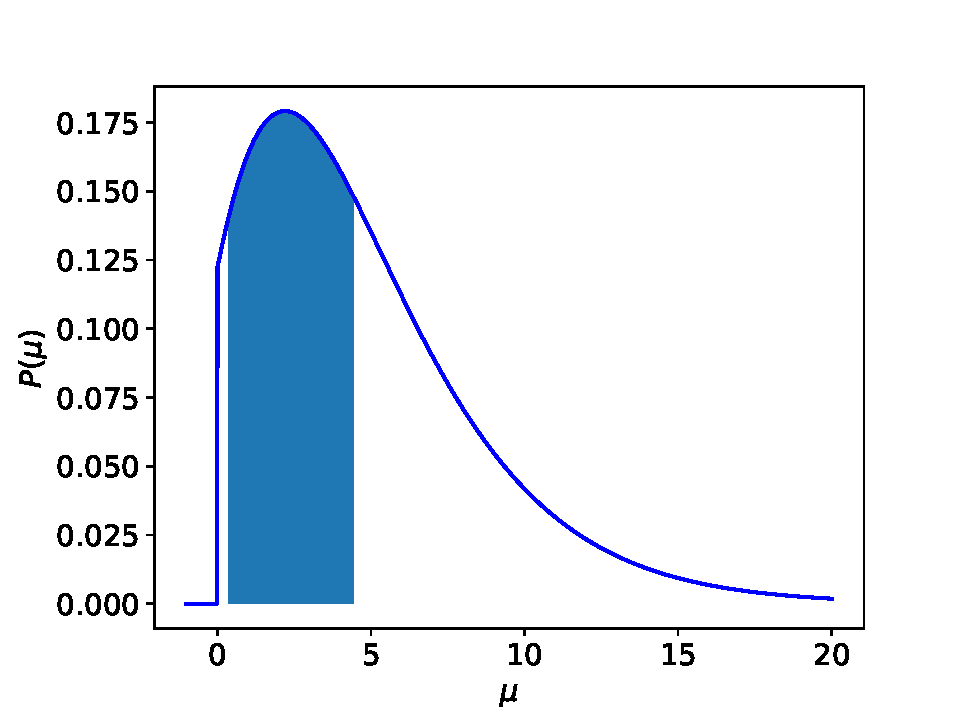
\includegraphics[width=0.8\textwidth]{figures/Intervals/credible_interval.pdf}
    \caption{Posterior $P(\mu)$ for the counting experiment, restricting $\mu>0$ in the prior for $\mu$. The shaded region indicates the shortest 68.3\% credible region.  }
    \label{fig:posterior_shortest_interval}
\end{figure}

In addition to choosing an interval, as always, studying the effect of changing priors $\pi(\mu)$ is a must for Bayesian credible intervals. So long as the data is powerful enough, $P(\mu)$ should be fairly insensitive to this choice -- but its not guaranteed! 
\section{Summary}
We're at the end of this short course on statistics for particle physics. Hopefully, some of the common terms in HEP that we mentioned in the first lecture are now clear. There are many other statistical concepts which we didn't have time to cover, and you may come across in your Ph.D,
\begin{itemize}
    \item Unfolding -- There are many publications on the issues of unfolding, removing detector effects to calculate cross-sections at particle level. 
    \item Information theory -- We touched on this when discussing Wilks' theorem (its related to the second derivative of the log-likelihood), but this is a whole topic unto itself. 
    \item Asymptotic theories -- Wilks' theorem is extremely powerful for determining intervals based on likelihood ratio test statistics, however, there are many other test statistics out there with well understood asymptotic behaviour. These may become more common as our computing gets more efficient. 
    \item Goodness of fits -- We covered a common goodness of fit test using likelihood ratios. There are many different tests that are sensitive to different ``features'' in the data. A good practise is to try several of them when checking the consistency of your models with the data. 
    \item Estimators -- We covered maximum likelihood estimators but there are others on the market, some more useful than others or have well known associated intervals.  
    \item Systematic uncertainties -- We only covered how to deal with systematic uncertainties as nuisance parameters, but estimating and dealing with systematic uncertainties in hypothesis testing is a huge field. Furthermore, we didn't cover the case where a parameter in the model isn't specified under one or more hypotheses. This can lead to something known as the \emph{Look elsewhere effect} and there are many interesting methods for dealing with this. 
\end{itemize}
There are several packages used by HEP collaborations that bundle common routines together and help make model building easier, 
\begin{itemize}
    \item \href{https://cds.cern.ch/record/1456844/files/CERN-OPEN-2012-016.pdf}{\textsf{HistFactory}} is used by the ATLAS collaboration, and comes with an XML based model builder for histogram based models. It is based on the \textsf{RooStats} libraries. There is a (almost complete) python based version too \href{https://scikit-hep.org/pyhf/}{\textsf{pyHF}}.
    \item \href{http://cms-analysis.github.io/HiggsAnalysis-CombinedLimit/}{\textsf{Combine}} is \emph{the} standard tool for statistical analysis for the CMS collaboration, using a text-based model definition. It is also based on \textsf{RooFit}, but includes several additional features and optimisations.
    \item \href{https://github.com/zfit/zfit}{\textsf{Zfit}} is a python based framework for building unbinned likelihoods, frequently used by the LHCb collaboration. 
\end{itemize}


Finally, the following is a list of recommended further reading to find out about some of these subjects and other issues in statistics pertinent for particle physics. 
\begin{itemize}
    \item L. Lyons, N. Wardle, ``\emph{Statistical issues in searches for new phenomena in High Energy Physics}'', Journal of Physics G: Nuclear and Particle Physics, Volume 45, Number 3. 
    \item  G. Cowan, ``Statistics'' (section 39) in ``\emph{Review of particle physics}'', Chin. Phys. C 40, 100001 (2016).
    \item O. Behnke, K. Kroninger, G. Schott, T.  Schorner-Sadenius, ``\emph{Data Analysis in High Energy Physics: A Practical Guide to Statistical Methods}'', ISBN: 978-3-527-41058-3 (2013).
    \item K. Cramner, ``\emph{Practical Statistics for the LHC}'', Proceedings, 2011 European School of High-Energy Physics, (2011).
    \item G. J. Feldman, R. D. Cousins, ``\emph{A Unified approach to the classical statistical analysis of small signals}'', Phys. Rev. D57 (1998).
    \item G. Cowan, ``\emph{Statistical Data Analysis}'', ISBN: 978-0-198-50155-8 (1998).
    \item L. Lista, ``\emph{Statistical Methods for Data Analysis in Particle Physics}'', ISBN 978-3-319-20176-4, (2015).
    \item F. James, ``\emph{Statistical Methods in Experimental Physics}'', ISBN: 978-9-812-70527-3 (2006). 
    \item A. Stuart, K. Ord, S. Arnold, ``\emph{Kendall's Advanced theory of Statistics}'', Vol 2A: Classical inference and the linear model, ISBN: 978-0-470-68924-0 (2010). 
\end{itemize}
\section{Problems}

\subsection{Kolmogorov axioms}

Show that the definitions of \emph{frequentist} and \emph{Bayesian} probabilities given in the lectures satisfy the three Kolmogorov axioms. 

\subsection{No correlation does not mean independence}

In the lectures, we said that two random variables which are independent will have a zero correlation coefficient. 

\begin{enumerate}
    \item Show that two continuous random variables $X$ and $Y$, with $(X,Y)\sim f(X,Y)$ which are independent will have a 0 correlation coefficient. 
    \item Let $X$ be a continuous random variable symmetrically distributed around 0 with a density function $f(X)$. Let $Y=X^{2}$. Show that despite the fact that $Y$ and $X$ are clearly dependent, their correlation coefficient is 0. 
\end{enumerate}

\subsection{Cauchy distribution}

In the lectures, we showed how the sum of two Gaussian distributed random variables is itself Gaussian distributed. Suppose now that $X\sim \phi(X;0,1)$ and  $Y\sim \phi(Y;0,1)$ are independent random variables. Show that the distribution of $Z=\dfrac{X}{Y}$ is Cauchy, i.e that $p(Z) = \dfrac{1}{\pi(1+Z^2)}$.

\textbf{Hint:} You should start by deriving the marginal distribution formula for the ratio of two independent random variables. Careful that the case $Y=0$ will cause a problem, so split the marginal distribution into two cases, one for $Y>0$ and one for $Y<0$. The sum of these marginal distributions will be the total distribution. 

\subsection{Convergence to a Dirac-delta function}

Let $X_{n}\sim\phi(X;0,1/n)$ for each $n$. Show that $X_{n}$ \emph{converges in distribution} to a probability density function which is a Dirac delta function at 0 $\delta(0)$. 

\textbf{Hint:} To show this, show that for any $X<0$, $F_{n}(X)\rightarrow 0$, and for any $X>0$, $F_{n}(X)\rightarrow 1$, as $n\rightarrow \infty$.


\subsection{Normal approximation to a Poisson}

Show that the Poisson probability density distribution $P(k)=\dfrac{\lambda^{k}}{k!}e^{-\lambda}$ converges (in distribution) to a normal probability density distribution as $\lambda\rightarrow\infty$. What are the mean and variance of the normal distribution that it converges to?

\textbf{Hint:} Start by considering a ``standardized'' Poisson random variable $K=\dfrac{k-\lambda}{\sqrt{\lambda}}$.

\subsection{Phone call for Peter Higgs}

You are sat at home with your statistics problems staring at you from across the room, and rather than solving them, you decide to procrastinate by dialing random telephone numbers. You punch a mobile number in only to have Peter Higgs himself pick up at the other end. What is the probability of picking Professor Higgs' number out of all possible UK mobile numbers? Is this more or less likely than the discovery of the Higgs boson being an accident due to a large fluctuation of the background?

\textbf{Hint:} You can assume the Higgs discovery was at exactly 5$\sigma$. Convert this to a $p$-value using a one-sided test as explained in lectures. Also use the fact that all UK mobile numbers are 11 digit numbers starting with 07. 

\subsection{Coverage of Poisson intervals}
Consider a simple Poisson process $k\sim \frac{\lambda^{k}}{k!}e^{-\lambda}$. The mean of the Poisson is $\lambda$ and its variance is $\sqrt{\lambda}$. Often, particle physicists will use this fact to ``measure'' $\lambda$, after observing $k$ events as $\lambda=k\pm\sqrt{k}$ -- i.e, claiming the range $[k-\sqrt{k},k+\sqrt{k}]$ as the 68.3\% interval. 

\begin{itemize}
    \item Calculate the coverage of this method for $\lambda$ in the range $\lambda\in[0.1,3]$ in steps of 0.1.
    \item Instead devise a method using a Neyman construction for the 68.3\% interval and calculate the coverage of that method in the same range.
\end{itemize}    

How do the coverage properties of the two methods to obtain a 68.3\% confidence interval compare?


\subsection{Maximum likelihood and intervals for exponential decay}

Suppose we want to determine the lifetime ($\tau$) of an unstable particle. The probability for this particle to decay at time $t$ is given by, 
\begin{equation}
    p(t) = N(\tau)e^{-t/\tau}
\end{equation}
Suppose then that in the lab, we've made measurements of the decay times (say by measuring the times at which we detect one or more decay products from a source), and have the following observed decay times; $t=$7.44, 4.13, 26.85, 1.42, 3.46, 2.68, 4.1, 4.04, 7.9 and 12.03 in ns.

\begin{enumerate}
\item Normalise the probability density function (i.e what is $N(\tau)$?)

\item What does the log-likelihood function look like for this dataset? Use your favourite plotting program to plot it as a function of $\tau$.  

\item What is the maximum likelihood (minimum negative log-likelihood) estimate for $\tau$? \textbf{Hint}: You can calculate this analytically or numerically (or even better, do both and compare answers).

\item Using Wilkes' theorem, estimate the 68.3\% confidence interval for $\tau$.

\item Derive a 68\% confidence interval for $\tau$ using the Neyman construction approach. You can use the profile likelihood ratio (as we did in lectures) as the test statistic for this. 

\end{enumerate}


\end{document}